\documentclass[12pt]{article}
\usepackage[margin=1in]{geometry}
\usepackage{float}
\usepackage{amsmath}
\usepackage{graphicx}
\usepackage{tikz-cd}
\usepackage{multicol}
\usepackage{xcolor}
\usepackage{setspace}
\usepackage{amssymb}
\usepackage{booktabs}
\usepackage{placeins}
\usepackage{todonotes}

% Bibliography (APA)
\usepackage{csquotes}
\usepackage[backend=biber,style=apa]{biblatex}
\addbibresource{master_thesis.bib}
\addbibresource{additional_pap.bib}

% --- Title page metadata (edit these) ---
\newcommand{\ThesisTitle}{Reinforcement Learning with NEAT in Multitask Environments}
\newcommand{\ThesisAuthor}{Sven Goerdes}
\newcommand{\ThesisDegree}{Master Thesis}
\newcommand{\ThesisProgram}{Your Program}
\newcommand{\ThesisUniversity}{Your University}
\newcommand{\ThesisDepartment}{Your Department / School}
\newcommand{\ThesisSupervisor}{Supervisor: Prof.\ Your Supervisor}
\newcommand{\ThesisCoSupervisor}{Co-supervisor: Dr.\ Your Co-supervisor}
\newcommand{\ThesisDate}{\today}

\setlength{\parindent}{0pt}
\setlength{\parskip}{1\baselineskip}
\onehalfspacing

% Show deeper levels in headings/ToC
\setcounter{secnumdepth}{3}
\setcounter{tocdepth}{3}

% Avoid huge unbreakable blocks when many headings appear consecutively
\makeatletter
\newcommand{\prism@clearafterheading}{\if@nobreak\mbox{}\par\fi}
\pretocmd{\section}{\prism@clearafterheading}{}{}
\pretocmd{\subsection}{\prism@clearafterheading}{}{}
\pretocmd{\subsubsection}{\prism@clearafterheading}{}{}
\makeatother

\begin{document}

\begin{titlepage}
  \thispagestyle{empty}
  \centering

  {\Large \ThesisUniversity\par}
  {\large \ThesisDepartment\par}
  \vfill

  {\LARGE\bfseries \ThesisTitle\par}
  \vspace{1.5cm}

  {\large \ThesisDegree\par}
  {\large \ThesisProgram\par}
  \vfill

  {\large \ThesisAuthor\par}
  \vspace{0.5cm}
  {\large \ThesisSupervisor\par}
  {\large \ThesisCoSupervisor\par}
  \vfill

  {\large \ThesisDate\par}
\end{titlepage}

\section*{Master Thesis Outline}

\tableofcontents

\bigskip

\newpage

\newpage

%\section{Introduction}
% =====================================================================
%  LITERATURE REVIEW  --  SKELETON  (fill-in scaffold, no prose yet)
% ---------------------------------------------------------------------
%  Red thread:
%    Neuroevolution  ->  NEAT (evolves topology)  ->  activation
%    functions  ->  HA-NEAT (evolves activation diversity)  ->  why
%    direct encoding  ->  continuous-control domain (Hopper/Walker2D)
%    ->  multi-task / one shared network  ->  the gap  ->  methodology
%
%  Legend inside each section:
%    PURPOSE  = one-line job of the section
%    COVER    = beats to hit
%    ANCHORS  = primary citation(s)
%    REUSE    = which of your existing paragraphs map here
%    ENDS     = the transition this section must land on
%
%  [TODO-CITE] marks bib keys you still need to add to the .bib file.
% =====================================================================

\section{Literature Review}


\subsection{Structural Differences in the Brain and in Artificial Neural Networks}


Unlike Artificial Neural Networks (ANNs), the human brain is a non-static and continuously changing network.
Neural cells form new connections throughout time and rewire to adapt to the current environment (\cite{pascualleone_plastic_2005,holtmaat_experience-dependent_2009}).
Cells are constantly rewiring and find new pathways to best represent the environment the human body is experiencing.
Human learning yields measurable structural plasticity, demonstrating that adaptation is supported by tangible architectural reconfiguration of the brain (\cite{draganski_changes_2004}).

In contrast, ANNs typically rely on static connections.
We create the structure of the neural network before we start training it.
Hence, the topology of the ANN is fixed.
Therefore, it is not possible for the ANN to create new connections while being trained.
We solely rely on adapting the weights of the ANN through a process called backpropagation (\cite{rumelhart_learning_1986}).
Inspired by biological learning, backpropagation can be seen as a simplified mathematical way to change synaptic strengths: the network keeps its wiring, but the "strength" of each connection is adjusted during training.
However, classical approaches with backpropagation do not allow us to adjust and change the topology of the ANNs.

Biological neurons also differ in their built-in response.
Two neurons can receive the same input and react differently, because their internal properties determine how each one transforms it (\cite{drion_ion_2015}).
This variety is functionally useful.
A population of differently responding neurons encodes information more effectively than a uniform one (\cite{tripathy_intermediate_2013}), and adding similar variety to artificial networks improves how well they learn (\cite{perez-nieves_neural_2021}).
A single activation function shared across every node discards this source of variety.



% ---------------------------------------------------------------------
% 1.2
% ---------------------------------------------------------------------
\subsection{Neuroevolution and the TWEANN Problem}
\label{subsec:neuroevolution}
% PURPOSE: introduce neuroevolution; motivate why evolving *topology*
%          (not only weights) is hard.
% COVER:
%   - neuroevolution = evolve the network instead of gradient-training it
%   - pre-NEAT TWEANN approaches                              [TODO-CITE]
%   - the hard parts: competing conventions / permutation problem,
%     crossover between unlike topologies, protecting young innovation,
%     starting dimensionality
% ANCHORS: \cite{stanley_evolving_2002} + 1-2 pre-NEAT TWEANNs  [TODO-CITE]
% REUSE:   the static-topology-vs-dynamic framing from your old
%          "Neuroevolution of augmenting topologies" opening.
% ENDS:    "...these problems are exactly what NEAT was built to solve."

% >>> write 1.1 here

An alternative approach to evolving ANNs is Neuroevolution.
Neuroevolution uses a evolutionary/genetic algorithm approach to design and train ANNs.
Selection crossover and mutation produce the next generation.
Not only can the connection weights change throughout the training process but also its topology.
Topology and weight evolving artificial neural networks (TWEANNs) are able to discover novel topological solutions and remove the manual design choice that one faces in the classical approach (\cite{stanley_designing_2019}).

% can we cite sth. here? 
% This just sounds really generic

A central obstacle for any method that evolves topology is that the same network function can be encoded by genomes whose nodes appear in different orders.
Because crossover recombines genomes by position, it can produce offspring that lose structures both parents possessed or that duplicate them incoherently.
Recombination then destroys the innovations it should preserve.
A method therefore needs a way to identify matching structure before combining genomes.

A second obstacle is the survival of new structure.
When a mutation adds a node or a connection, it almost always lowers fitness at first, because the new weights that have been added have not yet been optimized.
Such an innovation is out-competed and discarded before it can be tuned, even when the topology it introduces would ultimately prove valuable.
A TWEANN method therefore needs a way to give new structure time to mature before selection can eliminate it.

A third problem is that evolved topologies can grow without boundaries.
Many early TWEANNs added penalty terms to discourage bloat.
Such penalties however, are hard to tune and risk suppressing useful growth along with wasteful growth.
Therefore, we need to let a network add structure only when that structure earns its keep.

Earlier TWEANN methods addressed these three problems and controlling complexity only in part.
Neuroevolution of Augmenting Topologies (NEAT) (\cite{stanley_evolving_2002}) addresses all three at once.
It does so with a single coherent set of mechanisms.


% ---------------------------------------------------------------------
% 1.2
% ---------------------------------------------------------------------
\subsection{Neuroevolution of Augmenting Topologies (NEAT)}
% PURPOSE: how NEAT solves the TWEANN problem, via its three mechanisms.
% COVER:
%   (i)   historical markings / innovation numbers -> aligned crossover
%   (ii)  speciation via compatibility distance (delta) -> protects
%         innovation     [NB: define delta explicitly -- missing in draft]
%   (iii) minimal initialization + complexification -> low-dim search first
% ANCHORS: \cite{stanley_evolving_2002}
% REUSE:   most of your current NEAT subsection.
%          MOVE the HyperNEAT/CPPN paragraph OUT -> it now lives in 1.5.
% ENDS:    "...but every neuron's activation function stays fixed."

% >>> write 1.2 here

NEAT introduces a dynamic evolutionary based framework that optimizes both weights and network topology simultaneously (\cite{stanley_evolving_2002}).
It allows for the organic emergence of topological structures and starts out with a population of uniform ANNs with zero hidden nodes.
New structures (nodes and connections) are introduced with mutation throughout the evolutionary learning process.
This approach ensures that the algorithm starts searching for solutions in low dimensions first.

NEAT answers the three obstacles above with three mechanisms.
It assigns each new gene a global innovation number that is inherited unchanged.
Genes sharing a number encode the same structure, so NEAT aligns genomes during crossover without any prior topological analysis.
This solves the alignment problem.
To protect young structure, NEAT groups genomes into species by a compatibility distance and lets them compete mainly within their own species.
A fresh innovation then has time to be tuned before it faces the full population.
To control growth, NEAT starts from a minimal topology and adds nodes and connections only through mutation.
A network therefore expands only when the added structure survives selection, and no hand-tuned complexity penalty is needed. This incremental strategy keeps the search low-dimensional at the outset.
Scaling the evolved topologies to higher dimensions remains a challenge for NEATw.

Because NEAT optimises weights and topology by selection alone, it needs no gradient and no differentiable reward.
This suits continuous-control reinforcement learning, where the reward is delayed and non-differentiable.
NEAT evolves controllers directly from episodic returns and has been applied to control and locomotion tasks of the kind studied here (\cite{stanley_evolving_2002}).
The Hopper and Walker2D benchmarks used in this thesis belong to that setting.


% ---------------------------------------------------------------------
% 1.3
% ---------------------------------------------------------------------
\subsection{Activation Functions}
% PURPOSE: define the activation function as a design choice; show that
%          heterogeneity helps -- the groundwork HA-NEAT exploits.
% COVER:
%   - standard ANNs use one activation function across all nodes
%   - ReLU as canonical example (+ your tikz ReLU figure)
%   - mixed / heterogeneous activations beat homogeneous ones
%   - SANN: gradient-based precedent for per-neuron activation
%   - neuronal diversity outperforms homogeneous nets
% ANCHORS: \cite{nair_rectified_nodate}, \cite{krizhevsky_imagenet_2012},
%          \cite{dubey_activation_2022}, \cite{tutuncuoglu_neuronlevel_2025},
%          \cite{choudhary_neuronal_2023}   <- rescued citation
% REUSE:   your existing "Activation functions" subsection, near-verbatim,
%          including the ReLU tikz figure.
% DECISION: keep the one biological sentence (\cite{song_highly_2005},
%           synapse variation cell-to-cell) as light motivation, or cut it
%           for consistency with dropping the biology thread?
% ENDS:    "...so what if the activation function itself could evolve?"

% >>> write 1.3 here  (reuse ReLU figure)

% short explanation what activation functions are:

An activation function is the nonlinear transfer function applied at each neuron of an ANN.
Without them, a multilayer network reduces to a single linear map regardless of depth (\cite{dubey_activation_2022}).
Its choice governs a network's trainability and expressive power, and although many alternatives have been proposed, the Rectified Linear Unit (ReLU) remains the default in deep learning \cite{ramachandran_searching_2017}.
ReLU (\cite{nair_rectified_2010}) outputs zero for negative inputs and the input itself for positive ones, and it accelerates the convergence of stochastic gradient descent because its gradient is always one for positive inputs.



Common activation functions that are often used are the identity function $f(x)=x$, the sigmoid function $\sigma(x)=\frac{1}{1+e^{-x}}$, the hyperbolic tangent $\tanh(x)$, the Rectified Linear Unit $\mathrm{ReLU}(x)=\max(0,x)$, and the sine function $\sin(x)$.
These functions differ along the properties commonly used to characterise activation functions: output range, monotonicity, and smoothness (\cite{dubey_activation_2022}).
The sigmoid and the hyperbolic tangent are the classical choices, both bounded and saturating; the sigmoid maps to $(0,1)$ and $\tanh$ to the zero-centred interval $(-1,1)$ (\cite{dubey_activation_2022}).
Their saturation at large inputs later motivated the Rectified Linear Unit, which is piecewise-linear, unbounded above, and cheap to evaluate (\cite{nair_rectified_2010}).
ReLU has since become the default activation in deep learning; in deep convolutional networks such as AlexNet it accelerated training over saturating units (\cite{krizhevsky_imagenet_2012,ramachandran_searching_2017}).
The sine function is uncommon in feedforward training but has a longer history in neuroevolution, where periodic activations let a network encode repeating and symmetric structure compactly (\cite{stanley_compositional_2007}).
The identity function applies no nonlinearity.
A network of identity units collapses to a single linear map, the property that nonlinear activations exist to overcome (\cite{dubey_activation_2022}).
The choice of activation therefore shapes which mappings a network can represent and how efficiently it learns them (\cite{dubey_activation_2022}).
An overview of all those activation functions can be found below in Figure~\ref{fig:activation-functions}.

% \begin{figure}[h]\centering\begin{tikzpicture}[scale=0.9]  \draw[->] (-3,0) -- (3,0) node[right] {$x$};  \draw[->] (0,-0.5) -- (0,3) node[above] {$\mathrm{ReLU}(x)$};  \draw[thick] (-3,0) -- (0,0);  \draw[thick] (0,0) -- (3,3);\end{tikzpicture}\caption{Schematic plot of the Rectified Linear Unit (ReLU) activation function.}\label{fig:relu-plot}\end{figure}

\begin{figure}[h]
\centering
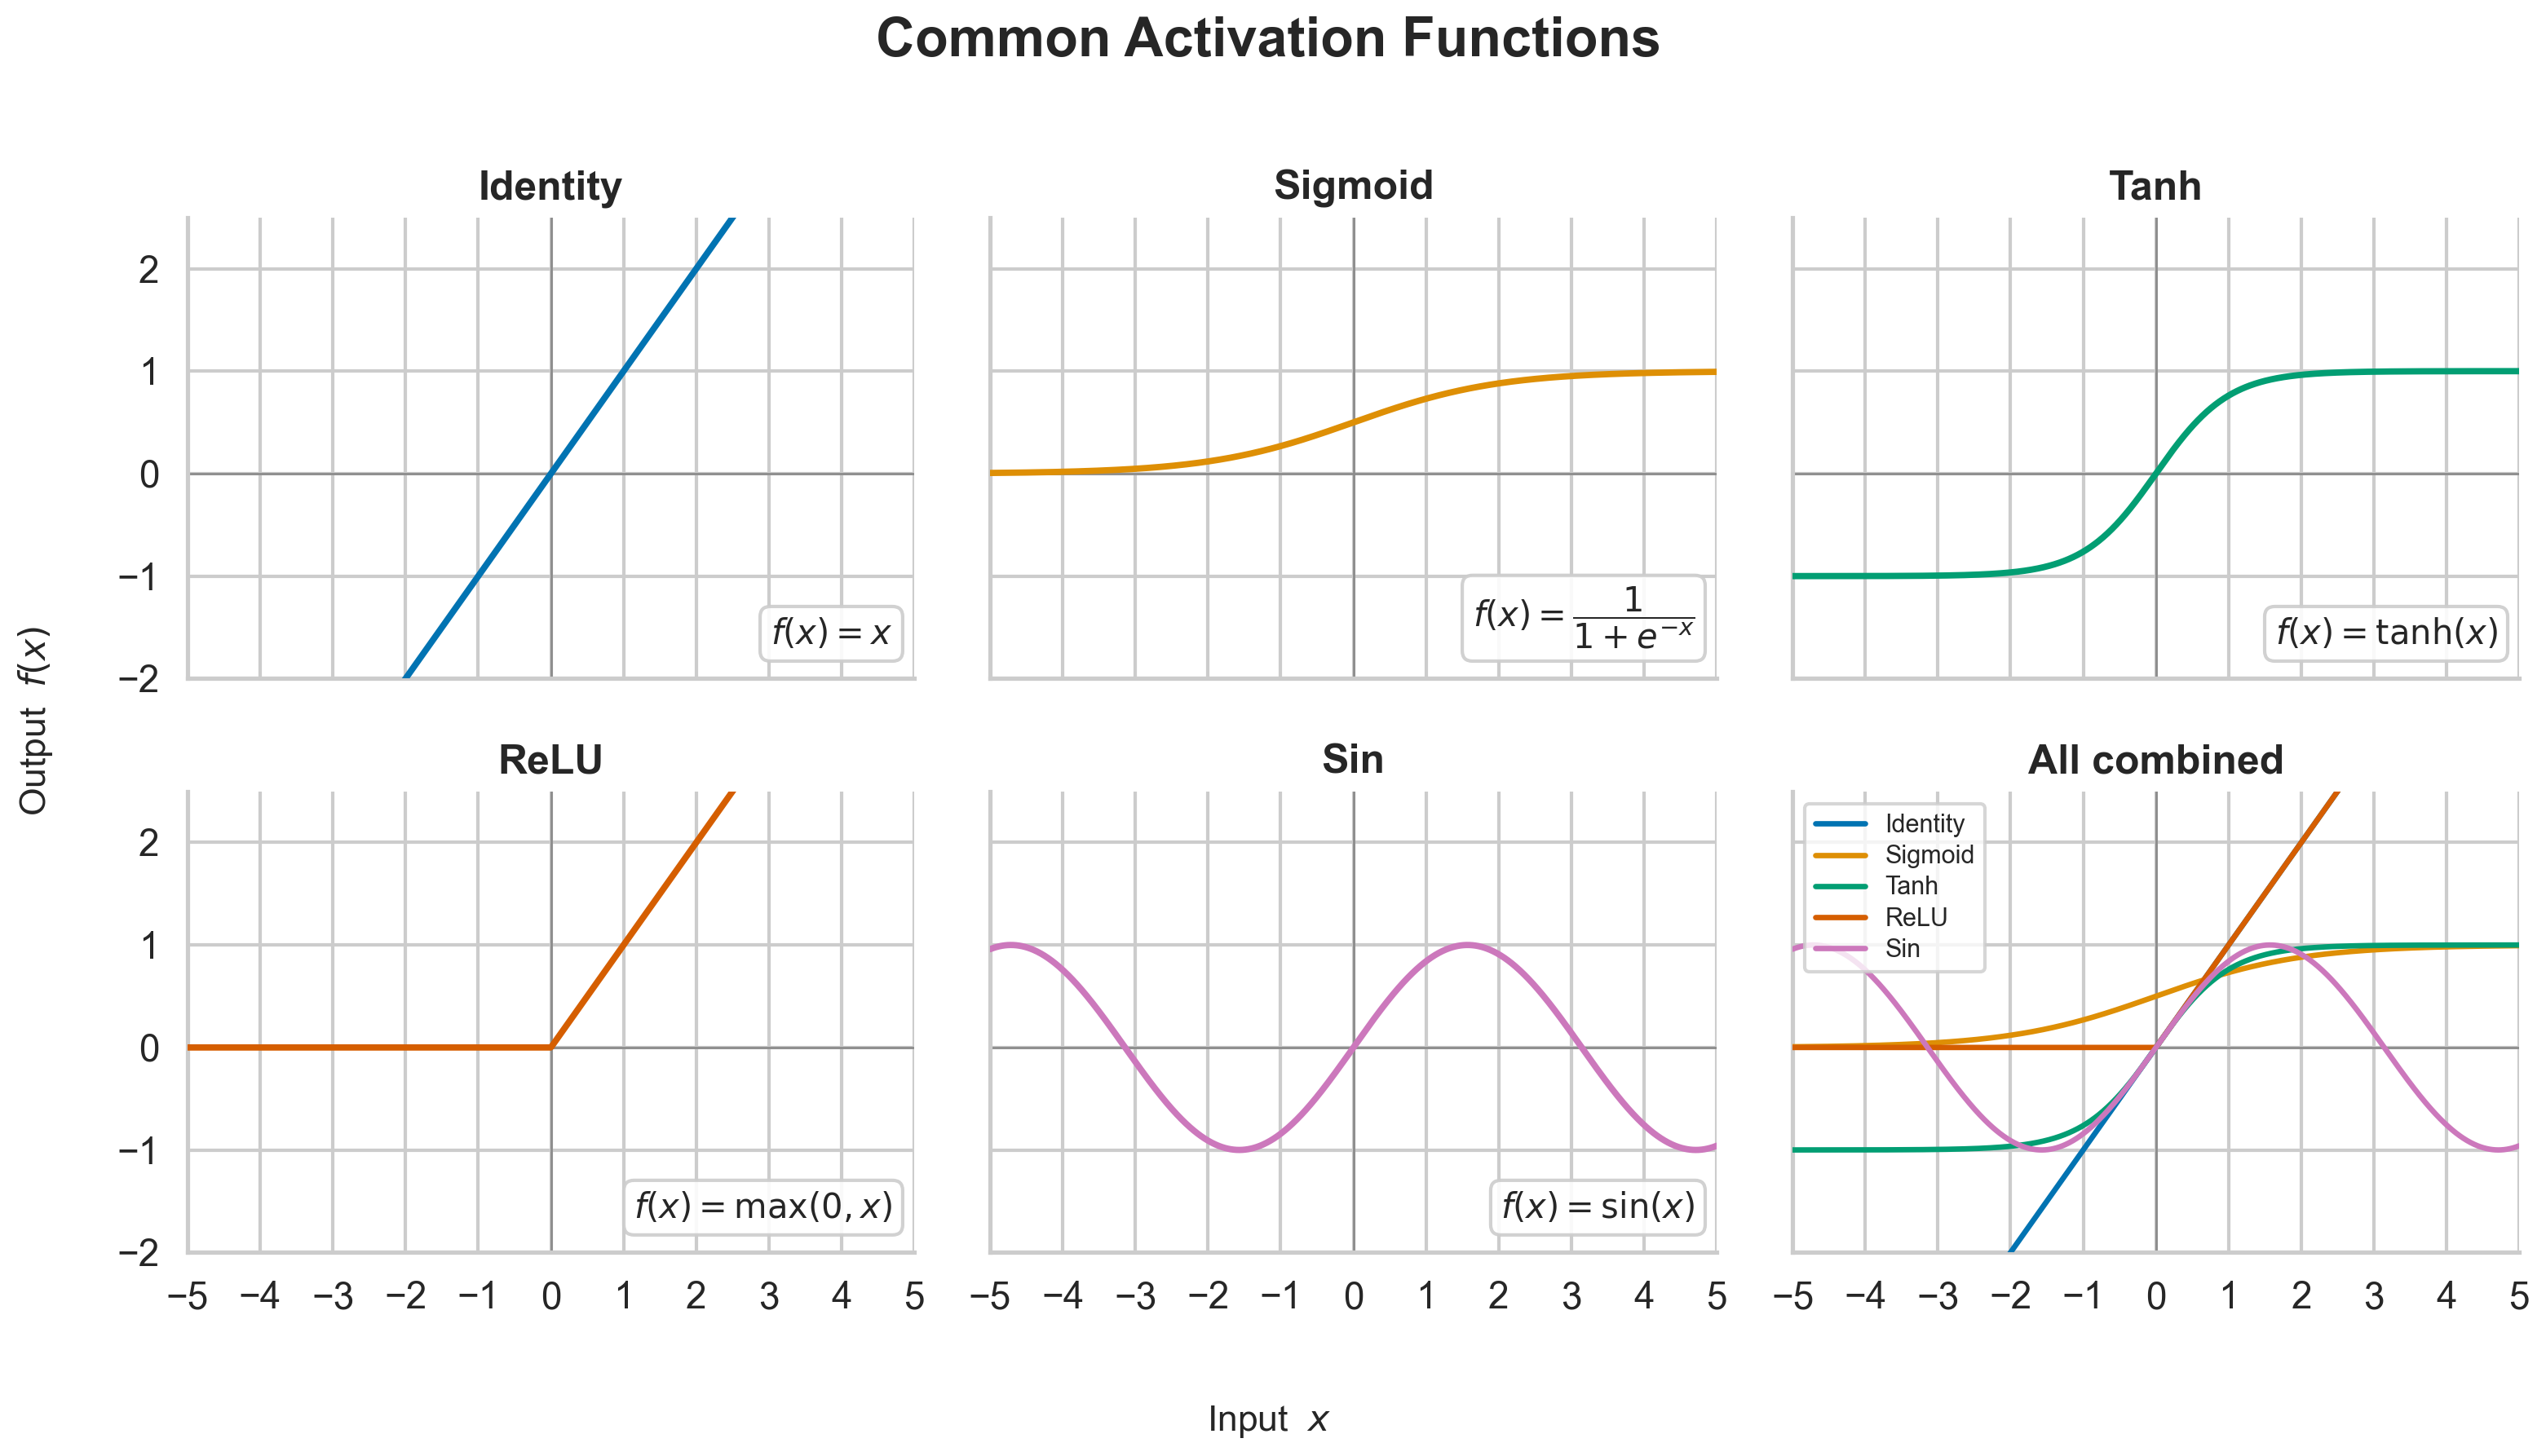
\includegraphics[width=0.85\textwidth]{Figures/activation_functions.png}
\caption{Comparison of common activation functions}
\label{fig:activation-functions}
\end{figure}

Artificial neural networks typically only use one activation function across every node (\cite{dubey_activation_2022}).
Biological neurons, in contrast, vary in their response properties even within a single cell type, and this diversity allows a population of neurons to encode roughly twice as much information as an equivalent homogeneous population (\cite{padmanabhan_intrinsic_2010}).

However, training a neural network with multiple activation functions (a heterogeneous network) has been shown to improve the performance of ANNs in different scenarios.
A comprehensive survey provided evidence that a mix of activation functions performs better than standard ReLU or sigmoid networks (\cite{dubey_activation_2022}).
Furthermore, a self-developing method called Self-Activating Neural Networks (SANN), which uses gradient descent to evolve a unique activation function for every neuron, shows that networks can represent functions that would otherwise require deeper architectures with fixed activation functions (\cite{tutuncuoglu_neuronlevel_2025}).
Standard NEAT, however, holds a single activation function fixed across every node, so the diversity that these results exploit is unavailable to it.
Making the activation function itself an evolvable, per-neuron trait is the extension that HA-NEAT introduces.


% Different problems need different mathematical transformations. 

%Creating neural networks with a diverse set of activation functions has shown to  Using a set of AF (relu, sigmoid, swish, tanh) instead of only one activation function can improve efficiency and decrease the size of the neural network. (add some examples here)

% ---------------------------------------------------------------------
% 1.4
% ---------------------------------------------------------------------
\subsection{Heterogeneous Neuroevolution (HA-NEAT)}
\label{subsec:haneat}
% PURPOSE: present HA-NEAT, its parsimony result, and its limitation.
% COVER:
%   - genome extension: per-neuron activation gene + mutation operator,
%     protected by speciation
%   - parsimony result: 50-70% smaller networks
%   - functional form changes inductive bias (FS-/FD-NEAT, HA-FD-NEAT)
%   - LIMITATION: all validated on static / classification data
% ANCHORS: \cite{hagg_evolving_2017}, \cite{papavasileiou_importance_2017},
%          \cite{papavasileiou_optimizing_2022}
% REUSE:   your "Heterogeneous Neuroevolution" subsection, nearly intact.
% ENDS:    "...but only on static data -- the continuous-control domain
%           is open."  (the domain gap)

% >>> write 1.4 here

The Heterogeneous Activation NEAT algorithm (HA-NEAT) (\cite{hagg_evolving_2017}) advances the standard NEAT algorithm.
It demonstrates empirically that heterogeneous networks achieve comparable or better accuracy than homogeneous ones while using fewer nodes and connections.
In their experiments, heterogeneous networks were often 50\%--70\% smaller in topological size than homogeneous baselines at matched accuracy.
To accomplish this, HA-NEAT adds to the traditional NEAT genome by encoding the activation function of each neuron as a specific gene.
This allowing the evolutionary process to select from a library of functions (e.g., Sine, Gaussian, ReLU) alongside topology and weights.
This approach introduces a new mutation operator that alters a node's activation function, utilizing NEAT's existing speciation mechanism to protect these potentially disruptive but innovative mathematical changes until they optimize.

In addition to structural parsimony (a preference for smaller networks with fewer nodes and connections), the choice of activation function is a critical aspect that significantly changes the inductive bias of a network.
\cite{papavasileiou_importance_2017} showed that the choice of functional form directly affects the discriminative ability of an algorithm.
The use of Gaussian output units in Feature Selective NEAT (FS-NEAT) and FD-NEAT enabled more accurate feature selection and the evolution of smaller topologies than Sigmoid or ReLU units.
This implies that the advantage of heterogeneity is not merely a consequence of size reduction but also a means of optimizing input processing.

In line with this, \cite{papavasileiou_optimizing_2022} proposed HA-FD-NEAT, which evolves the heterogeneity, topology, and input selection of a neural network.
The results of their study show that the synchronization of a neuron's properties with its connectivity enables the evolution of a particular task's inductive bias.
The identification of optimal architectures is seemingly dependent on this combination, in which functional diversity is a means of both topological compression and accurate feature relevance.


% ---------------------------------------------------------------------
% 1.5
% ---------------------------------------------------------------------
\subsection{Direct and Indirect Encoding}
% PURPOSE: justify staying with NEAT's direct, parsimonious encoding.
% COVER:
%   - direct (NEAT/HA-NEAT): explicit genome, parsimony, per-neuron
%     activation control, interpretable
%   - indirect (HyperNEAT/CPPN): abstracts connectivity from geometry,
%     scales to millions of connections, but loses per-neuron control and
%     assumes geometric regularity that locomotion does not offer
%   - why direct encoding fits this thesis
% ANCHORS: \cite{stanley_hypercubebased_2009}, \cite{stanley_compositional_2007}
%          (used here as CONTRAST, not as the chosen method)
% REUSE:   the HyperNEAT/CPPN paragraph relocated out of 1.2, reframed.
% ENDS:    "...therefore this work stays with direct encoding."

% >>> write 1.5 here

Neuroevolution methods differ in how a genome maps to a network.
NEAT uses a direct encoding, in which every node, connection, and (in HA-NEAT) activation function appears explicitly in the genome, so that genotype and phenotype grow together.
Direct encoding gives three properties this work depends on: parsimony is measurable and under selective control, each neuron's activation can be set individually, and the evolved network remains interpretable.
Indirect encodings break this correspondence.

HyperNEAT \cite{stanley_hypercubebased_2009} evolves a Compositional Pattern-Producing Network (CPPN) \cite{stanley_compositional_2007} that computes each connection weight from the geometric coordinates of its endpoints, so a small genome can describe substrates with millions of connections.
The abstraction has costs in this setting.
The substrate's neurons no longer carry individually specified activation functions.
Phenotype size is also decoupled from the genome, so parsimony can no longer be measured directly from what evolves.
The encoding's benefit further rests on geometric regularity, the spatial structure that a visual field provides but that the low-dimensional proprioceptive state of Hopper and Walker2D does not.
Its scaling advantage is in any case irrelevant at this size, since locomotion controllers need far fewer connections than the regime in which direct encodings become impractical \cite{stanley_hypercubebased_2009}.
Because this work requires per-neuron activation control and parsimony as a directly measured quantity, and because its environments offer little geometry for an indirect encoding to exploit, it stays with direct encoding.

% ---------------------------------------------------------------------
% 1.6
% ---------------------------------------------------------------------
\subsection{Continuous-Control Benchmarks}
\label{subsec:control-benchmarks}
% PURPOSE: introduce the domain and why it is harder than where
%          (HA-)NEAT was validated.
% COVER:
%   - continuous-control locomotion benchmarks
%   - Hopper and Walker2D  (state here: 11 / 17 observations, 3 / 6 actions)
%   - why harder than classification: high-dim continuous actions,
%     temporal credit assignment, policy-dependent non-stationary state
%     distribution, no labels
%   - MuJoCo locomotion lineage
%   - Brax = JAX reimplementation -> massively parallel evaluation
%     (why this matters for population-based neuroevolution); TensorNEAT
% ANCHORS: \cite{freeman_brax_2021}      [TODO-CITE]
%          \cite{todorov_mujoco_2012}    [TODO-CITE]
%          \cite{brockman_openai_2016}   [TODO-CITE]
%          TensorNEAT                     [TODO-CITE]
% REUSE:   nothing from the old Meta-World text.
% ENDS:    "...yet heterogeneous-activation neuroevolution has never been
%           tested in this domain."

% >>> write 1.6 here

Continuous-control locomotion benchmarks evaluate a policy that outputs real-valued torques for a simulated articulated body.
The standard suite originates in the MuJoCo physics engine (\cite{todorov_mujoco_2012}), whose fast and accurate contact dynamics made physically grounded locomotion tasks tractable for reinforcement-learning research.
Two of its canonical tasks anchor this thesis.
Hopper is a one-legged body that must hop forward without falling; its state is an $11$-dimensional vector of joint positions and velocities, and its action is a $3$-dimensional torque vector, one per actuated joint.
Walker2D is a planar biped that must walk forward while balancing on two legs; it exposes a $17$-dimensional observation and a $6$-dimensional action.
The two bodies share a kinematic lineage: Walker2D is essentially Hopper's leg mirrored into a pair, so one of its legs reproduces the same thigh--leg--foot chain that constitutes the whole of Hopper.
This overlap is what makes a single shared controller a plausible target for the two tasks.

These tasks are qualitatively harder than the static classification, regression, and low-dimensional toy control settings in which HA-NEAT has historically been validated \cite{hagg_evolving_2017}.
Three properties account for the difficulty.
The action space is high-dimensional and continuous, so the controller outputs real-valued torques instead of a discrete label.
Reward arrives only after a sequence of actions, so credit must be assigned across time.
And the distribution of states the policy encounters is itself a function of the policy, which makes the learning target non-stationary and unlabelled.
A controller that performs well must therefore encode temporally coherent behaviour over an episode.

Population-based neuroevolution is expensive in this domain because every genome must be rolled out over full episodes to estimate its fitness.
Brax (\cite{freeman_brax_2021}) reduces this cost by reimplementing MuJoCo-style locomotion in JAX, so that thousands of environment instances run in parallel on a single accelerator and evaluation compiles onto the same device as the search.
This shift made population-based evaluation on locomotion tractable at scales that were previously impractical.
The search algorithm must match that scale.
Classical CPU-bound NEAT libraries do not reach the population sizes and generation counts this study requires.
GPU-native implementations such as TensorNEAT (\cite{wang_tensorized_2024}) close the gap by tensorising the evolutionary operators onto the same accelerator that runs the simulation.

Despite the maturity of these benchmarks, heterogeneous-activation neuroevolution has never been tested in this domain: its parsimony and inductive-bias advantages remain established only on static data.


% ---------------------------------------------------------------------
% 1.7
% ---------------------------------------------------------------------
\subsection{Multi-Task Learning with a Single Shared Network}
% NOTE: title deliberately avoids "Reinforcement Learning" -- your
%       professor flagged that the old title was not about RL methods.
% PURPOSE: introduce multi-task learning as related work; motivate one
%          shared controller for two environments (evolutionary framing,
%          NOT gradient-based MTRL as *your* method).
% COVER:
%   - multi-task RL landscape as contrast (gradient MTRL, engineered
%     expert modules)
%   - the neuroevolutionary alternative
%   - why one shared network is the harder / more interesting target
%   - shared-network rationale: zero-padded 28-in / 9-out union;
%     Walker2D right-leg ~ Hopper leg kinematic overlap
% ANCHORS: \cite{mclean_multitask_2025}     [TODO-CITE]
%          \cite{hendawy_multitask_2024}    [TODO-CITE]
%          \cite{zhang_mixture--world_2026} (gradient-MTRL contrast)
%          \cite{zhou_neuroevolutionary_2024} [TODO-CITE] (closest
%            evolutionary precedent)
%          \cite{leng_understanding_2025}         <- rescued citation
% REUSE:   essentially new; old Meta-World prose does not survive.
% DECISION: preview the zero-padding mechanics here, or keep 1.7
%           conceptual and detail them in Methodology?
%           (recommendation: keep conceptual here.)
% ENDS:    "...and never as a single shared network."

% >>> write 1.7 here

Multi-task learning is a paradigm where a single model is trained on multiple related tasks simultaneously.
By sharing representations and learning processes, the knowledge gained from one task can help improve the performance and generalization of the others (\cite{zhang_survey_2021}).
Recent empirical analysis of Large Language Models (LLMs) reveals that powerful generalist models naturally develop ``task-specific neurons'' that specialize in distinct functional roles (\cite{leng_understanding_2025}).
This thesis hypothesizes that by providing a set of activation functions, evolution can explicitly assign these specialized mathematical ``personalities'' to specific neurons, thereby organically modularizing the control policy.

To evaluate the efficacy of heterogeneous activation functions in high-dimensional continuous control, this research uses two Brax locomotion environments (\cite{freeman_brax_2021}): Hopper and Walker2D.
A single evolved network must control both bodies at once using one shared set of weights.
The two tasks require diverse motor skills, from single-leg hopping to bipedal balance and forward propulsion.
This setting is suited for this study because the two environments differ in observation dimensionality and body dynamics, challenging a single genome to generalize across both.
While approaches such as Mixture-of-World (MoW) models address this heterogeneity by explicitly engineering diverse expert modules (\cite{zhang_mixtureofworld_2026}), this thesis posits that a heterogeneous neural network based on the NEAT algorithm can emergently discover similar functional modularity by evolving a diverse population of neurons tailored to the two locomotion tasks.

% ---------------------------------------------------------------------
% 1.8
% ---------------------------------------------------------------------
\subsection{Research Gap and Contribution}
% PURPOSE: synthesize 1.4 x 1.6 (x 1.7) into the gap; state the
%          contribution; hand off to the methodology.
% COVER:
%   - the gap = heterogeneous-activation neuroevolution (static-data only)
%     INTERSECT multi-task continuous-control locomotion (never done this way)
%   - contribution: one shared neuroevolved network, heterogeneous
%     per-neuron activations, Hopper + Walker2D SIMULTANEOUSLY;
%     the JAX / Brax / TensorNEAT pipeline
%   - the "activation personalities" hypothesis (modularizing the policy)
% ANCHORS: synthesis of 1.4 + 1.6 + 1.7; your own hypothesis
% REUSE:   your "This thesis hypothesizes..." paragraph lands cleanly here.
% ENDS:    "...which sets up the methodology that follows."

% >>> write 1.8 here

Two lines of work meet in this thesis.
Heterogeneous-activation neuroevolution (Section~\ref{subsec:haneat}) shows that letting evolution choose a per-neuron activation function yields smaller networks and a task-adapted inductive bias.
Every such result, however, has been established on static, single-task classification data.
Continuous-control locomotion (Section~\ref{subsec:control-benchmarks}) is a mature benchmark domain for neuroevolution, yet it has only ever been approached with a homogeneous activation function fixed across all nodes.
Whether activation heterogeneity confers an advantage in a temporally extended control setting remains an open question.
The same holds for \emph{emergent modularity}: the spontaneous specialisation of neurons within a single shared network that must solve more than one task at once.
That intersection is the gap this thesis addresses.

% TODO(intro): when the Introduction is written, move this contribution paragraph
% there and reduce this subsection to the gap statement above (retitle to "Research Gap").
The contribution is a single shared network whose per-neuron activations are heterogeneous and evolved.
One such network controls Hopper and Walker2D at once, over the union of both tasks' observation and action spaces: the smaller observation is zero-padded and the unused actions are sliced away.
A GPU-native evolutionary pipeline makes population-based evaluation feasible at this scale.
We hypothesise that a library of activation functions lets evolution assign distinct mathematical ``personalities'' to individual neurons, and that this specialisation modularises the control policy across the two tasks without engineered expert modules.
The following chapter specifies the shared-network encoding, the activation library, and the evolutionary protocol used to test this hypothesis.


% =====================================================================
%  [ OPEN SLOT ]  Additional topics you mentioned go here. Send the
%  titles + anchor papers and I will insert / renumber them without
%  breaking the red thread.
% =====================================================================

% \section{Literature Review}

% \subsection{Activation functions}
% Artificial neural networks typicall only use one activation functions across every node. In biological neural networks, the synapses between two cells vary from cell to cell (\cite{song_highly_2005}). ANNs, on the other hand, typically use the very same activation function in one single across the  network. 

% An activation function that is often used, because of its simplicity and its properties, is the Rectified Linear Unit (ReLU) (\cite{nair_rectified_nodate}). ReLU outputs 0 for negative inputs and the input itself for positive inputs. Mathematically, it is defined as $\mathrm{ReLU}(x)=\max(0,x)$. ReLu can accelerate the convergence of Stochastic Gradient Descend, as its gradient is always one for positive inputs. This allows the network to learn faster. A simple ANN trained on the CIFAR-10 dataset achieved six times faster a 25\% training error rate than using the tanh function (\cite{krizhevsky_imagenet_2012}). Figure~\ref{fig:relu-plot} shows a schematic plot of this function. 

% \begin{figure}[h]\centering\begin{tikzpicture}[scale=0.9]  \draw[->] (-3,0) -- (3,0) node[right] {$x$};  \draw[->] (0,-0.5) -- (0,3) node[above] {$\mathrm{ReLU}(x)$};  \draw[thick] (-3,0) -- (0,0);  \draw[thick] (0,0) -- (3,3);\end{tikzpicture}\caption{Schematic plot of the Rectified Linear Unit (ReLU) activation function.}\label{fig:relu-plot}\end{figure}

% \newpage

% % Different problems need different mathematical transformations. 
% However, training a neural network with multiple activation functions (heterogeneous network) has shown to improve the performance of ANNs in different scenarious. A comprehensive survey provided evidence that a mix of activation functions performs better than standard ReLu or sigmoid networks (\cite{dubey_activation_2022}). Furthermore, a self developing method called Self-Activating Neural Networks (SANN) that uses gradient descend to evole a unique AF for every Neuron shows that networks can theoretically represent functions that would otherwise require deeper architectures with fixed activation functions (\cite{tutuncuoglu_neuronlevel_2025}).

% %Creating neural networks with a diverse set of activation functions has shown to  Using a set of AF (relu, sigmoid, swish, tanh) instead of only one activation function can improve efficiency and decrease the size of the neural network. (add some examples here)

% \subsection{Neuroevolution of augmenting topoflogies}

% Typical ANNs stick to the initialized topology and then adjust their weights throughout the training process. Thus, we are stuck optimizing weights for a pre-determined structure. In contrast to this static approach, the Neuroevolution of Augmenting Topologies algorithm (NEAT) introduces a dynamic evolutionary based framework that optimizes both synaptic weights and network topology simultaneously (\cite{stanley_evolving_2002}). The NEAT algorithm is based on evolutionary learning theory. It allows for the organic emergence of topological structures and starts out with a population of uniform ANNs with zero hidden nodes. New structures (nodes and connections) are introduced with mutation throughout the learning process. This approach ensures that the algorithm starts searching for solutions in low dimensions first

% To manage the increasing structural diversity between the ANNs, NEAT utilizes historical markings to align gene crossover between differing topologies. Additionally, it employs speciation to protect new topological innovations, allowing new structures to survive and develope before competing against other solutions of the population.

% While NEAT starts out with a small search spaces by starting with minimal topology, scaling to higher dimensions remains a challenge. To overcome this bottleneck, \cite{stanley_hypercubebased_2009} introduced Hypercube-based NeuroEvolution of Augmenting Topologies (HyperNEAT), which utilizes an indirect encoding method based on Compositional Pattern Producing Networks (CPPNs) (\cite{stanley_compositional_2007}). A CPPN operates as a mapping system where geometric coordinates, such as x and y, serve as inputs to determine the output at that specific location. Unlike standard neural networks that typically use a single activation function, CPPNs utilize a diverse set of functions like gaussian, sine, and sigmoid. This variety enables the network to capture geometric regularities like symmetry and repetition. By exploiting the geometric regularities of the task domain HyperNEAT abstracts the connectivity pattern rather than optimizing each connection individually. This allows the algorithm to enable the evolution of functional networks with millions of connections. 

% \subsection{Heterogeneous Neuroevolution}
% The Heterogeneous Activation NEAT algorithm (HA-NEAT) (\cite{hagg_evolving_2017}) advances the standard NEAT algorithm. It proves empirically that heterogeneous ANNs are structuraly more efficient than bigger ones. The integration of diverse activation functions enables more efficient neural networks. A smaller neural network (less nodes and weights) produces similar or even better accuracy than bigger neural networks with homogenous activation functions. In their experiments, hetergoenous networks were often 50\% - 70\% smaller (in terms of topological size) compared to homogenous baselines. To accomplish this, HA-NEAT adds to the traditional NEAT genome by encoding the activation function of each neuron as a specific gene. This allowing the evolutionary process to select from a library of functions (e.g., Sine, Gaussian, ReLU) alongside topology and weights. This approach introduces a new mutation operator that alters a node's activation function, utilizing NEAT's existing speciation mechanism to protect these potentially disruptive but innovative mathematical changes until they optimize.

% In addition to structural parsimony, the choice of activation function is a critical aspect that significantly changes the inductive bias of a network. \cite{papavasileiou_importance_2017} showed that the choice of functional form directly affects the discriminative ability of an algorithm. The use of Gaussian output units in Feature Selective NEAT (FS-NEAT) and FD-NEAT enabled more accurate feature selection and the evolution of smaller topologies than Sigmoid or ReLU units. This implies that the advantage of heterogeneity is not merely a consequence of size reduction but also a means of optimizing input processing.

% In line with this, \cite{papavasileiou_optimizing_2022} proposed HA-FD-NEAT, which evolves the heterogeneity, topology, and input selection of a neural network. The results of their study show that the synchronization of a neuron's properties with its connectivity enables the evolution of a particular task's inductive bias. The identification of optimal architectures is seemingly dependent on this combination, in which functional diversity is a means of both topological compression and accurate feature relevance.




%Compositional Pattern Producing Networks (CPPNs) offer a robust method for abstracting biological development. They encode complex spatial patterns without the need to simulate local interactions or growth over time. A CPPN operates as a mapping system where geometric coordinates, such as x and y, serve as inputs to determine the output at that specific location . Unlike standard neural networks that typically use a single activation function, CPPNs utilize a diverse set of functions like Gaussian, sine, and sigmoid. This variety enables the network to capture geometric regularities like symmetry and repetition. Additionally, because the phenotype is defined by a continuous function, patterns can be represented at infinite resolution

%To bridge the gap between smaller and complex neural networks \cite{stanley_compositional_2007} introduced Compositional Pattern Producing Networks (CPPNs). 

%Hypercube based NEAT (HyperNEAT) introduces a algorithm that uses indirect encoding to approach this problem \cite{stanley_hypercubebased_2009}. It evolves a pattern-producing network that itself generates the weights of the final Network that is used to solve the problem.

% \subsection{Multi-Task Reinforcement Learning}
% This thesis hypothesizes that by providing a diverse library of activation functions, evolution can explicitly assign these specialized mathematical "personalities" to specific neurons, thereby organically modularizing the control policy. 

% To evaluate the efficacy of heterogeneous activation functions in high-dimensional continuous control, this research makes use of the Meta-World benchmark (\cite{yu_meta-world_2021}). Meta-World presents a suite of 50 distinct robotic manipulation tasks (MT50) that share a common physical simulated robot arm. It requires the acquisition of diverse motor skills, ranging from precise pick-and-place operations to dynamic object manipulation. 

% The benchmark is suited for this study because it introduces significant heterogeneity in both observation spaces and task dynamics, challenging the agent to generalize across different environments. While state-of-the-art approaches like Mixture-of-World (MoW) models address this heterogeneity by explicitly engineering diverse expert modules (\cite{zhang_mixture--world_2026}), this thesis posits that an Heterogenous Neural Network based on the NEAT algorithm can emergently discover similar functional modularity by evolving a diverse population of neurons tailored to specific sub-tasks within the Meta-World environment.

% \section{Literature Review}
% \subsection{Neuroplasticity}
% Unlike Artificial Neural Networks (ANNs), the (human) brain is a non-static and continuously changing network. Neural cells form new connections throughout time and rewire to adapt to the current environment (\cite{pascualleone_plastic_2005,holtmaat_experience-dependent_2009}). Cells are constantly rewiring and find new pathways to best represent the environment the human body is experiencing. Human learning yields measurable structural plasticity, demonstrating that adaptation is supported by tangible architectural reconfiguration of the brain (\cite{draganski_changes_2004}). 

% Neuro-plasiticy is the reason why animals and humans are able to learn new behaviours and patterns through experience. It describes the process of neural networks forming. Human brain cells are able to create new connections between each other. (\cite{hebb_organization_1949}, \cite{bliss_lomo_1973})

% In contrast, ANNs typically rely on static connections. We create the structure of the neural, network before we start training it. Hence, the topology of the ANN is fixed. Therefore, it is not possible for artificial intelligence (AI) to create new connections to different neurons while being trained. We solely rely on adapting the weights of the ANN through a process called backpropagation (\cite{rumelhart_learning_1986}). Inspired by biological learning, backpropagation can be seen as a simplified mathematical way to change synaptic strengths: the network keeps its wiring, but the "strength" of each connection is adjusted during training. In the brain, synaptic change is also not random but gated by local activity and chemical signals, which provides a useful inspiration even if the biological mechanism is not identical to backpropagation (\cite{fremaux_neuromodulated_2016,roelfsema_three-factor_2018}). 

% Gradient descend tries to find an optimal solution where a loss function is minimized. This training regime works well when data is available in large batches and the task distribution is mostly stationary. However, the underlying data often changes its distribution throughout time (data shift), which is common in real-world environments and can lead to ANNs whose learned statistical assumptions become outdated (\cite{quinonero-candela_dataset_2009,gama_survey_2014}).


% \subsection{Catastrophic Forgetting}
% Another difference between ANNs and classical neura networks becomes visible once tasks arrive sequentially. Homogeneous ANNs tend to overwrite previously learned representations (Catastrophic forgetting), whereas biological systems maintain a much richer toolbox of mechanisms to protect and reorganize knowledge over time. Catastrophic forgetting (also called catastrophic interference) describes the tendency of gradient-based ANNs to lose performance on previously learned tasks when trained sequentially on new tasks. Early analyses suggest that this is not a minor side-effect but a structural property of distributed representations: when multiple tasks share parameters, learning task $B$ will typically move weights into a region that is no longer optimal for task $A$ (\cite{mccloskey_catastrophic_1989,french_catastrophic_1999}). In practice, this makes "learning from a stream" fundamentally different from the standard independent identically distributed (i.i.d.) setting that most deep learning pipelines assume.

% In machine learning, this gap motivates continual learning methods that explicitly reduce forgetting (\cite{kirkpatrick_overcoming_2017,parisi_continual_2019}) and approaches that re-introduce fast, local plasticity into networks, i.e., making parts of the connectivity itself adapt online (\cite{miconi_differentiable_2018}). \cite{lillo_activation_2026} found that the AF choice is an "architecture-agnostic lever for mitigating plasticity loss" in continual learning setting. Furthermore, mathematical and neuronal diversity, much like that observed in biological systems, significantly outperforms homogeneous architectures by enhancing the expressiveness and adaptability of artificial neural networks. (\cite{choudhary_neuronal_2023}). 

% While catastrophic forgetting is often introduced on supervised benchmarks, it becomes particularly relevant in reinforcement learning. The data distribution is non-stationary because it depends on the current policy, and even small updates can change the visited state distribution. This makes stability-plasticity trade-offs harder and increases the pressure on replay, regularization, and modular architectures (\cite{khetarpal_continual_2020,schwarz_progress_2018}).

% %From a continual learning perspective, modern approaches can be roughly grouped into (i) rehearsal/replay, (ii) regularization-based stabilization, and (iii) architectural strategies. Replay methods keep a small memory buffer (or a generative model) and interleave old experiences with new ones, which is conceptually close to what is done in many RL agents via experience replay (\cite{rolnick_experience_2019}). Regularization-based methods, such as Elastic Weight Consolidation (EWC), constrain updates along directions that are estimated to be important for past tasks (\cite{kirkpatrick_overcoming_2017}), while related methods like Synaptic Intelligence track parameter importance online (\cite{zenke_continual_2017}). Architectural strategies reduce interference by allocating new capacity over time, for example via progressive networks that grow task-specific modules while preserving earlier ones (\cite{rusu_progressive_2016}). Knowledge-distillation based methods, such as Learning without Forgetting, fit naturally into this picture by retaining old function outputs while adapting to a new dataset (\cite{li_learning_2017}).



% \subsection{Activation functions}
% Artificial neural networks typicall only use one activation functions across every node. In biological neural networks, the synapses between two cells vary from cell to cell (\cite{song_highly_2005}). ANNs, on the other hand, typically use the very same activation function in one single across the  network. 

% An activation function that is often used, because of its simplicity and its properties, is the Rectified Linear Unit (ReLU) (\cite{nair_rectified_nodate}). ReLU outputs 0 for negative inputs and the input itself for positive inputs. Mathematically, it is defined as $\mathrm{ReLU}(x)=\max(0,x)$. ReLu can accelerate the convergence of Stochastic Gradient Descend, as its gradient is always one for positive inputs. This allows the network to learn faster. A simple ANN trained on the CIFAR-10 dataset achieved six times faster a 25\% training error rate than using the tanh function (\cite{krizhevsky_imagenet_2012}). Figure~\ref{fig:relu-plot} shows a schematic plot of this function. 

% \begin{figure}[h]\centering\begin{tikzpicture}[scale=0.9]  \draw[->] (-3,0) -- (3,0) node[right] {$x$};  \draw[->] (0,-0.5) -- (0,3) node[above] {$\mathrm{ReLU}(x)$};  \draw[thick] (-3,0) -- (0,0);  \draw[thick] (0,0) -- (3,3);\end{tikzpicture}\caption{Schematic plot of the Rectified Linear Unit (ReLU) activation function.}\label{fig:relu-plot}\end{figure}

% \newpage

% % Different problems need different mathematical transformations. 
% However, training a neural network with multiple activation functions (heterogeneous network) has shown to improve the performance of ANNs in different scenarious. A comprehensive survey provided evidence that a mix of activation functions performs better than standard ReLu or sigmoid networks (\cite{dubey_activation_2022}). Furthermore, a self developing method called Self-Activating Neural Networks (SANN) that uses gradient descend to evole a unique AF for every Neuron shows that networks can theoretically represent functions that would otherwise require deeper architectures with fixed activation functions (\cite{tutuncuoglu_neuronlevel_2025}).

% %Creating neural networks with a diverse set of activation functions has shown to  Using a set of AF (relu, sigmoid, swish, tanh) instead of only one activation function can improve efficiency and decrease the size of the neural network. (add some examples here)

% Another key difference becomes visible once tasks arrive sequentially: standard ANNs tend to overwrite previously learned representations (catastrophic forgetting), whereas biological systems maintain a much richer toolbox of mechanisms to protect and reorganize knowledge over time. In machine learning, this gap motivates continual learning methods that explicitly reduce forgetting (\cite{kirkpatrick_overcoming_2017,parisi_continual_2019}) and approaches that re-introduce fast, local plasticity into networks, i.e., making parts of the connectivity itself adapt online (\cite{miconi_differentiable_2018}). \cite{lillo_activation_2026} found that the AF choice is an "architecture-agnostic lever for mitigating plasticity loss" in continual learning setting. Furthermore, neuronal diversity like in biological systems has shown evidence to outperform homogenous ones (\cite{choudhary_neuronal_2023})

% \subsection{Neuroevolution of augmenting topologies}

% Typical ANNs stick to the initialized topology and then adjust their weights throughout the training process. Thus, we are stuck optimizing weights for a pre-determined structure. In contrast to this static approach, the Neuroevolution of Augmenting Topologies algorithm (NEAT) introduces a dynamic evolutionary based framework that optimizes both synaptic weights and network topology simultaneously (\cite{stanley_evolving_2002}). The NEAT algorithm is based on evolutionary learning theory. It allows for the organic emergence of topological structures and starts out with a population of uniform ANNs with zero hidden nodes. New structures (nodes and connections) are introduced with mutation throughout the learning process. This approach ensures that the algorithm starts searching for solutions in low dimensions first

% To manage the increasing structural diversity between the ANNs, NEAT utilizes historical markings to align gene crossover between differing topologies. Additionally, it employs speciation to protect new topological innovations, allowing new structures to survive and develope before competing against other solutions of the population.

% While NEAT starts out with a small search spaces by starting with minimal topology, scaling to higher dimensions remains a challenge. To overcome this bottleneck, \cite{stanley_hypercubebased_2009} introduced Hypercube-based NeuroEvolution of Augmenting Topologies (HyperNEAT), which utilizes an indirect encoding method based on Compositional Pattern Producing Networks (CPPNs) (\cite{stanley_compositional_2007}). A CPPN operates as a mapping system where geometric coordinates, such as x and y, serve as inputs to determine the output at that specific location. Unlike standard neural networks that typically use a single activation function, CPPNs utilize a diverse set of functions like gaussian, sine, and sigmoid. This variety enables the network to capture geometric regularities like symmetry and repetition. By exploiting the geometric regularities of the task domain HyperNEAT abstracts the connectivity pattern rather than optimizing each connection individually. This allows the algorithm to enable the evolution of functional networks with millions of connections. 

% \subsection{Heterogeneous Neuroevolution}
% The Heterogeneous Activation NEAT algorithm (HA-NEAT) (\cite{hagg_evolving_2017}) advances the standard NEAT algorithm. It proves empirically that heterogeneous ANNs are structuraly more efficient than bigger ones. The integration of diverse activation functions enables more efficient neural networks. A smaller neural network (less nodes and weights) produces similar or even better accuracy than bigger neural networks with homogenous activation functions. In their experiments, hetergoenous networks were often 50\% - 70\% smaller (in terms of topological size) compared to homogenous baselines. To accomplish this, HA-NEAT adds to the traditional NEAT genome by encoding the activation function of each neuron as a specific gene. This allowing the evolutionary process to select from a library of functions (e.g., Sine, Gaussian, ReLU) alongside topology and weights. This approach introduces a new mutation operator that alters a node's activation function, utilizing NEAT's existing speciation mechanism to protect these potentially disruptive but innovative mathematical changes until they optimize.

% In addition to structural parsimony, the choice of activation function is a critical aspect that significantly changes the inductive bias of a network. \cite{papavasileiou_importance_2017} showed that the choice of functional form directly affects the discriminative ability of an algorithm. The use of Gaussian output units in Feature Selective NEAT (FS-NEAT) and FD-NEAT enabled more accurate feature selection and the evolution of smaller topologies than Sigmoid or ReLU units. This implies that the advantage of heterogeneity is not merely a consequence of size reduction but also a means of optimizing input processing.

% In line with this, \cite{papavasileiou_optimizing_2022} proposed HA-FD-NEAT, which evolves the heterogeneity, topology, and input selection of a neural network. The results of their study show that the synchronization of a neuron's properties with its connectivity enables the evolution of a particular task's inductive bias. The identification of optimal architectures is seemingly dependent on this combination, in which functional diversity is a means of both topological compression and accurate feature relevance.




% %Compositional Pattern Producing Networks (CPPNs) offer a robust method for abstracting biological development. They encode complex spatial patterns without the need to simulate local interactions or growth over time. A CPPN operates as a mapping system where geometric coordinates, such as x and y, serve as inputs to determine the output at that specific location . Unlike standard neural networks that typically use a single activation function, CPPNs utilize a diverse set of functions like Gaussian, sine, and sigmoid. This variety enables the network to capture geometric regularities like symmetry and repetition. Additionally, because the phenotype is defined by a continuous function, patterns can be represented at infinite resolution

% %To bridge the gap between smaller and complex neural networks \cite{stanley_compositional_2007} introduced Compositional Pattern Producing Networks (CPPNs). 

% %Hypercube based NEAT (HyperNEAT) introduces a algorithm that uses indirect encoding to approach this problem \cite{stanley_hypercubebased_2009}. It evolves a pattern-producing network that itself generates the weights of the final Network that is used to solve the problem.

% \subsection{Multi-Task Reinforcement Learning}
% The transition from homogeneous to heterogeneous architectures is necessitated by the "stability-plasticity dilemma," where standard neural networks suffer from catastrophic forgetting as learning new tasks interferes with the weights required for previous ones (\cite{abbasi_sparsity_2022}). Recent empirical analysis of Large Language Models (LLMs) supports this view, revealing that powerful generalist models naturally develop "task-specific neurons" that specialize in distinct functional roles (\cite{leng_understanding_2025}). 

% This thesis hypothesizes that by providing a diverse library of activation functions, evolution can explicitly assign these specialized mathematical "personalities" to specific neurons, thereby organically modularizing the control policy. 

% To evaluate the efficacy of heterogeneous activation functions in high-dimensional continuous control, this research makes use of the Meta-World benchmark (\cite{yu_meta-world_2021}). Meta-World presents a suite of 50 distinct robotic manipulation tasks (MT50) that share a common physical simulated robot arm. It requires the acquisition of diverse motor skills, ranging from precise pick-and-place operations to dynamic object manipulation. 

% The benchmark is suited for this study because it introduces significant heterogeneity in both observation spaces and task dynamics, challenging the agent to generalize across different environments. While state-of-the-art approaches like Mixture-of-World (MoW) models address this heterogeneity by explicitly engineering diverse expert modules (\cite{zhang_mixture--world_2026}), this thesis posits that an Heterogenous Neural Network based on the NEAT algorithm can emergently discover similar functional modularity by evolving a diverse population of neurons tailored to specific sub-tasks within the Meta-World environment.



%Contemporary deep learning predominantly relies on gradient-based optimization methods, such as backpropagation, applied to fixed, pre-defined network topologies. While this paradigm has achieved remarkable success in supervised learning, it inherently assumes that the initialized architecture possesses the optimal inductive bias for the given task.

%In contrast to this static approach, the Neuroevolution of Augmenting Topologies  algorithm introduces a dynamic evolutionary based framework that optimizes both synaptic weights and network topology simultaneously (\cite{stanley_evolving_2002}). Unlike gradient-based methods, NEAT begins with minimal complexity and incrementally adds nodes and connections. 

%While gradient methods typically offer superior sample efficiency in high-dimensional parameter spaces, NEAT provides a distinct advantage in reinforcement learning environments characterized by sparse rewards or deceptive local optima. Crucially, by uncoupling the agent from rigid architectural constraints, NEAT allows for the organic emergence of topological structures, providing a fertile ground for investigaZting how specialized functional modules might evolve without explicit human design.

%While canonical NEAT excels at optimizing topology, it typically relies on a homogeneous set of activation functions—usually sigmoids—thereby assuming a uniform non-linearity suffices for all processing tasks. Addressing this limitation, \cite{hagg_evolving_2017} proposed Heterogeneous Activation NEAT (HA-NEAT), an extension that co-evolves the activation function of individual neurons alongside the network structure and weights. By expanding the genome to include a direct encoding of diverse activation types—such as Gaussian, ReLU, Step, and Sigmoid—HA-NEAT allows the evolutionary process to select the most appropriate local inductive bias for specific network regions. This heterogeneity encourages greater parsimony, producing significantly smaller networks that are less prone to overfitting than their homogeneous counterparts. Crucially for multi-task domains, this diversity facilitates emergent modularity; for example, distinct activation profiles allow the network to organically separate correlated signals into distinct functional pathways, a phenomenon observed where specific sub-networks specialize in partial aspects of the target output.


\section{Methodology}

\subsection{Problem Formulation}

This work addresses the multi-task learning problem of evolving a single neuroevolutionary network capable of controlling two continuous-locomotion agents simultaneously: Hopper and Walker2D from the Brax physics suite.
The objective is a single shared neural network that receives observations from either environment, generates the appropriate joint-torque actions, and accumulates reward across both tasks, in place of two separately trained controllers.
A genome's fitness is therefore defined by its combined performance on both environments, evaluated every generation.

The two agents were introduced in Section~\ref{subsec:control-benchmarks}; the dimensions that drive the shared-network design are what matter here.
Hopper exposes an 11-dimensional observation and a 3-dimensional action, while Walker2D exposes a 17-dimensional observation and a 6-dimensional action.
The mismatch in these dimensions is the reason a single fixed-topology network cannot ingest both environments directly, and it motivates the padding scheme described below.
The two bodies also share kinematics: Walker2D's right leg reproduces Hopper's thigh--leg--foot chain.
This overlap gives evolution a reason to discover shared locomotion primitives, so a single network is a principled design choice for these two tasks.

The central hypothesis is twofold.
First, it is hypothesised that a multi-task evaluation regime enables implicit transfer between tasks: representations acquired on Hopper's simpler locomotion problem can bootstrap performance on Walker2D, and vice versa.
Second, it is hypothesised that heterogeneous activation functions within the network enable richer internal representations than homogeneous networks, improving the capacity for cross-task generalisation.
Both claims are tested through a controlled comparison of standard NEAT against HA-NEAT (Heterogeneous Activation NEAT) in the multi-task setting.

\subsection{Algorithm Design: HA-NEAT}

\subsubsection{Conceptual Motivation}

Before presenting the formal algorithmic details, it is useful to consider the intuition behind heterogeneous activations.
A locomotion controller must simultaneously encode qualitatively different computations: periodic oscillations for gait timing, saturating thresholds for balance, and proportional responses for joint control.
In a standard NEAT network, every hidden node applies the same activation function, typically $\tanh$, and the network must approximate all of these behaviours through compositions of a single nonlinearity, potentially requiring more nodes and connections than a heterogeneous network.
HA-NEAT addresses this by allowing each hidden node to carry its own activation function drawn from a diverse palette.
However, per-node activation changes can be disruptive, and a newly mutated genome risks elimination before its weights co-adapt.
HA-NEAT therefore pairs activation diversity with a speciation-based protection mechanism, described below.

\subsubsection{NEAT Foundation}

NEAT (NeuroEvolution of Augmenting Topologies) evolves both the topology and the weights of neural networks through three core mechanisms: historical marking of genes for alignment during crossover, speciation to protect structural innovation, and complexification from minimal initial topologies.
The algorithm is well established in the literature and is summarised here only to the extent necessary to contextualise the HA-NEAT extensions.

Each genome encodes a variable-topology neural network as two gene lists: node genes and connection genes.
A node gene stores a unique index, a bias value, an aggregation function, and an activation function.
A connection gene stores source and destination node indices, a historical marker, and a weight value.
In the TensorNEAT implementation used in this work, active genes occupy the first rows of fixed-size arrays; inactive positions are filled with NaN.
This padding convention enables batched operations across a population of genomes with different topologies under JAX's static-shape compilation model.

The population is partitioned into species based on genetic distance.
For each pair of genomes, the distance function aligns connection genes by historical marker, counts non-homologous (disjoint and excess) genes, and computes attribute differences on homologous genes.
Formally, the distance between two genomes is defined as:

$$d = \frac{D \cdot c_d + \sum_{i \in H} \delta_i \cdot c_w}{\max(n_1, n_2)}$$

where $D$ denotes the count of non-homologous genes, $H$ denotes the set of homologous gene pairs, $\delta_i$ is the attribute distance for pair $i$, $c_d = 1.0$ and $c_w = 0.4$ are coefficients weighting disjoint and weight differences respectively, and $n_1$, $n_2$ are the gene counts of each genome.
Genomes whose distance falls below the compatibility threshold $\theta = 1.0$ are assigned to the same species.

Within each species, the top fraction of genomes, determined by the survival threshold, produces offspring through crossover and mutation.
During crossover, the fitter parent contributes the structural backbone; homologous genes are inherited randomly from either parent, while all non-homologous genes (disjoint and excess) are inherited from the fitter parent.

\subsubsection{HA-NEAT Extensions}

HA-NEAT extends the standard NEAT algorithm with three modifications, all encapsulated within the mutation operator.
The speciation-driven evolutionary loop, crossover, and distance computation remain unchanged.
Each modification is described in turn.

\begin{enumerate}
    \item \textbf{Random activation assignment upon node creation.} In standard NEAT, a newly added node receives an identity activation function, making the structural mutation initially neutral. HA-NEAT instead assigns a random activation function drawn uniformly from $\mathcal{A} = \{\tanh, \sigma, \text{ReLU}, \sin, \text{identity}\}$ at node creation. This introduces immediate functional diversity: the new node contributes a non-trivial transformation from its first generation, avoiding the evolutionary delay of waiting for a separate activation mutation.
    
    \item \textbf{Controlled activation mutation with speciation protection.} With probability $p_{\text{act}} = 0.1$ per genome per generation, exactly one randomly selected hidden node has its activation function replaced by a function selected from
    $\mathcal{A}$ with equal probability across all elements of the palette. Upon this mutation, all connections incident to the mutated node receive new historical markers from a pre-allocated pool, increasing the genetic distance between the mutated genome and its relatives. This causes the speciation mechanism to place the mutant into a separate species, protecting it from competitive elimination before its weights can co-adapt to the new activation landscape.
    
    The marker reassignment requires pre-allocating $3 + C_{\max}$ historical markers per genome per generation, where $C_{\max}$ denotes the maximum number of connections. The first three markers serve standard structural mutations; the remaining $C_{\max}$ cover the worst-case connections incident to any single node. This scheme avoids dynamic memory allocation within the JAX computation graph, which requires static shapes at compilation time.
    
    \item \textbf{Suppression of standard activation mutation.} Standard NEAT applies per-node activation mutation with independent probability during value mutation. HA-NEAT disables this mechanism: the activation column is saved before value mutation and restored afterward, ensuring that only the controlled one-node-per-generation mechanism modifies activations. Unprotected activation changes, i.e. those without corresponding marker reassignment, would lack the speciation shield, exposing functionally disrupted genomes to immediate competitive pressure.
\end{enumerate}

\subsubsection{Genome Representation and the Padding Scheme}

Because Hopper and Walker2D differ in observation and action dimensionality, a mechanism is required to present both environments to a single fixed-topology network.
The approach adopted in this work is a union padding scheme: the network is constructed with 17 input nodes and 6 output nodes, corresponding to the maximum observation and action dimensions across both tasks.
This design was chosen over modular sub-networks to keep the transfer learning argument clean: any shared structure discovered by evolution arises from optimisation pressure alone, not from architectural induction bias.

Formally, given a network $f: \mathbb{R}^{17} \rightarrow \mathbb{R}^{6}$, the task-specific action functions are defined as:

$$a_{\text{Hopper}} = f([\mathbf{o}_{\text{Hopper}}; \mathbf{0}_{6}])_{1:3}$$
$$a_{\text{Walker}} = f(\mathbf{o}_{\text{Walker}})_{1:6}$$

where $[\cdot; \cdot]$ denotes concatenation and the subscript denotes output slicing.
For Hopper, the 11-dimensional observation vector is zero-padded to 17 dimensions before being presented to the network, and only the first 3 of the 6 output dimensions are used as actions.
For Walker2D, all inputs and outputs are used directly without modification.

\begin{figure}[h]
    \centering
    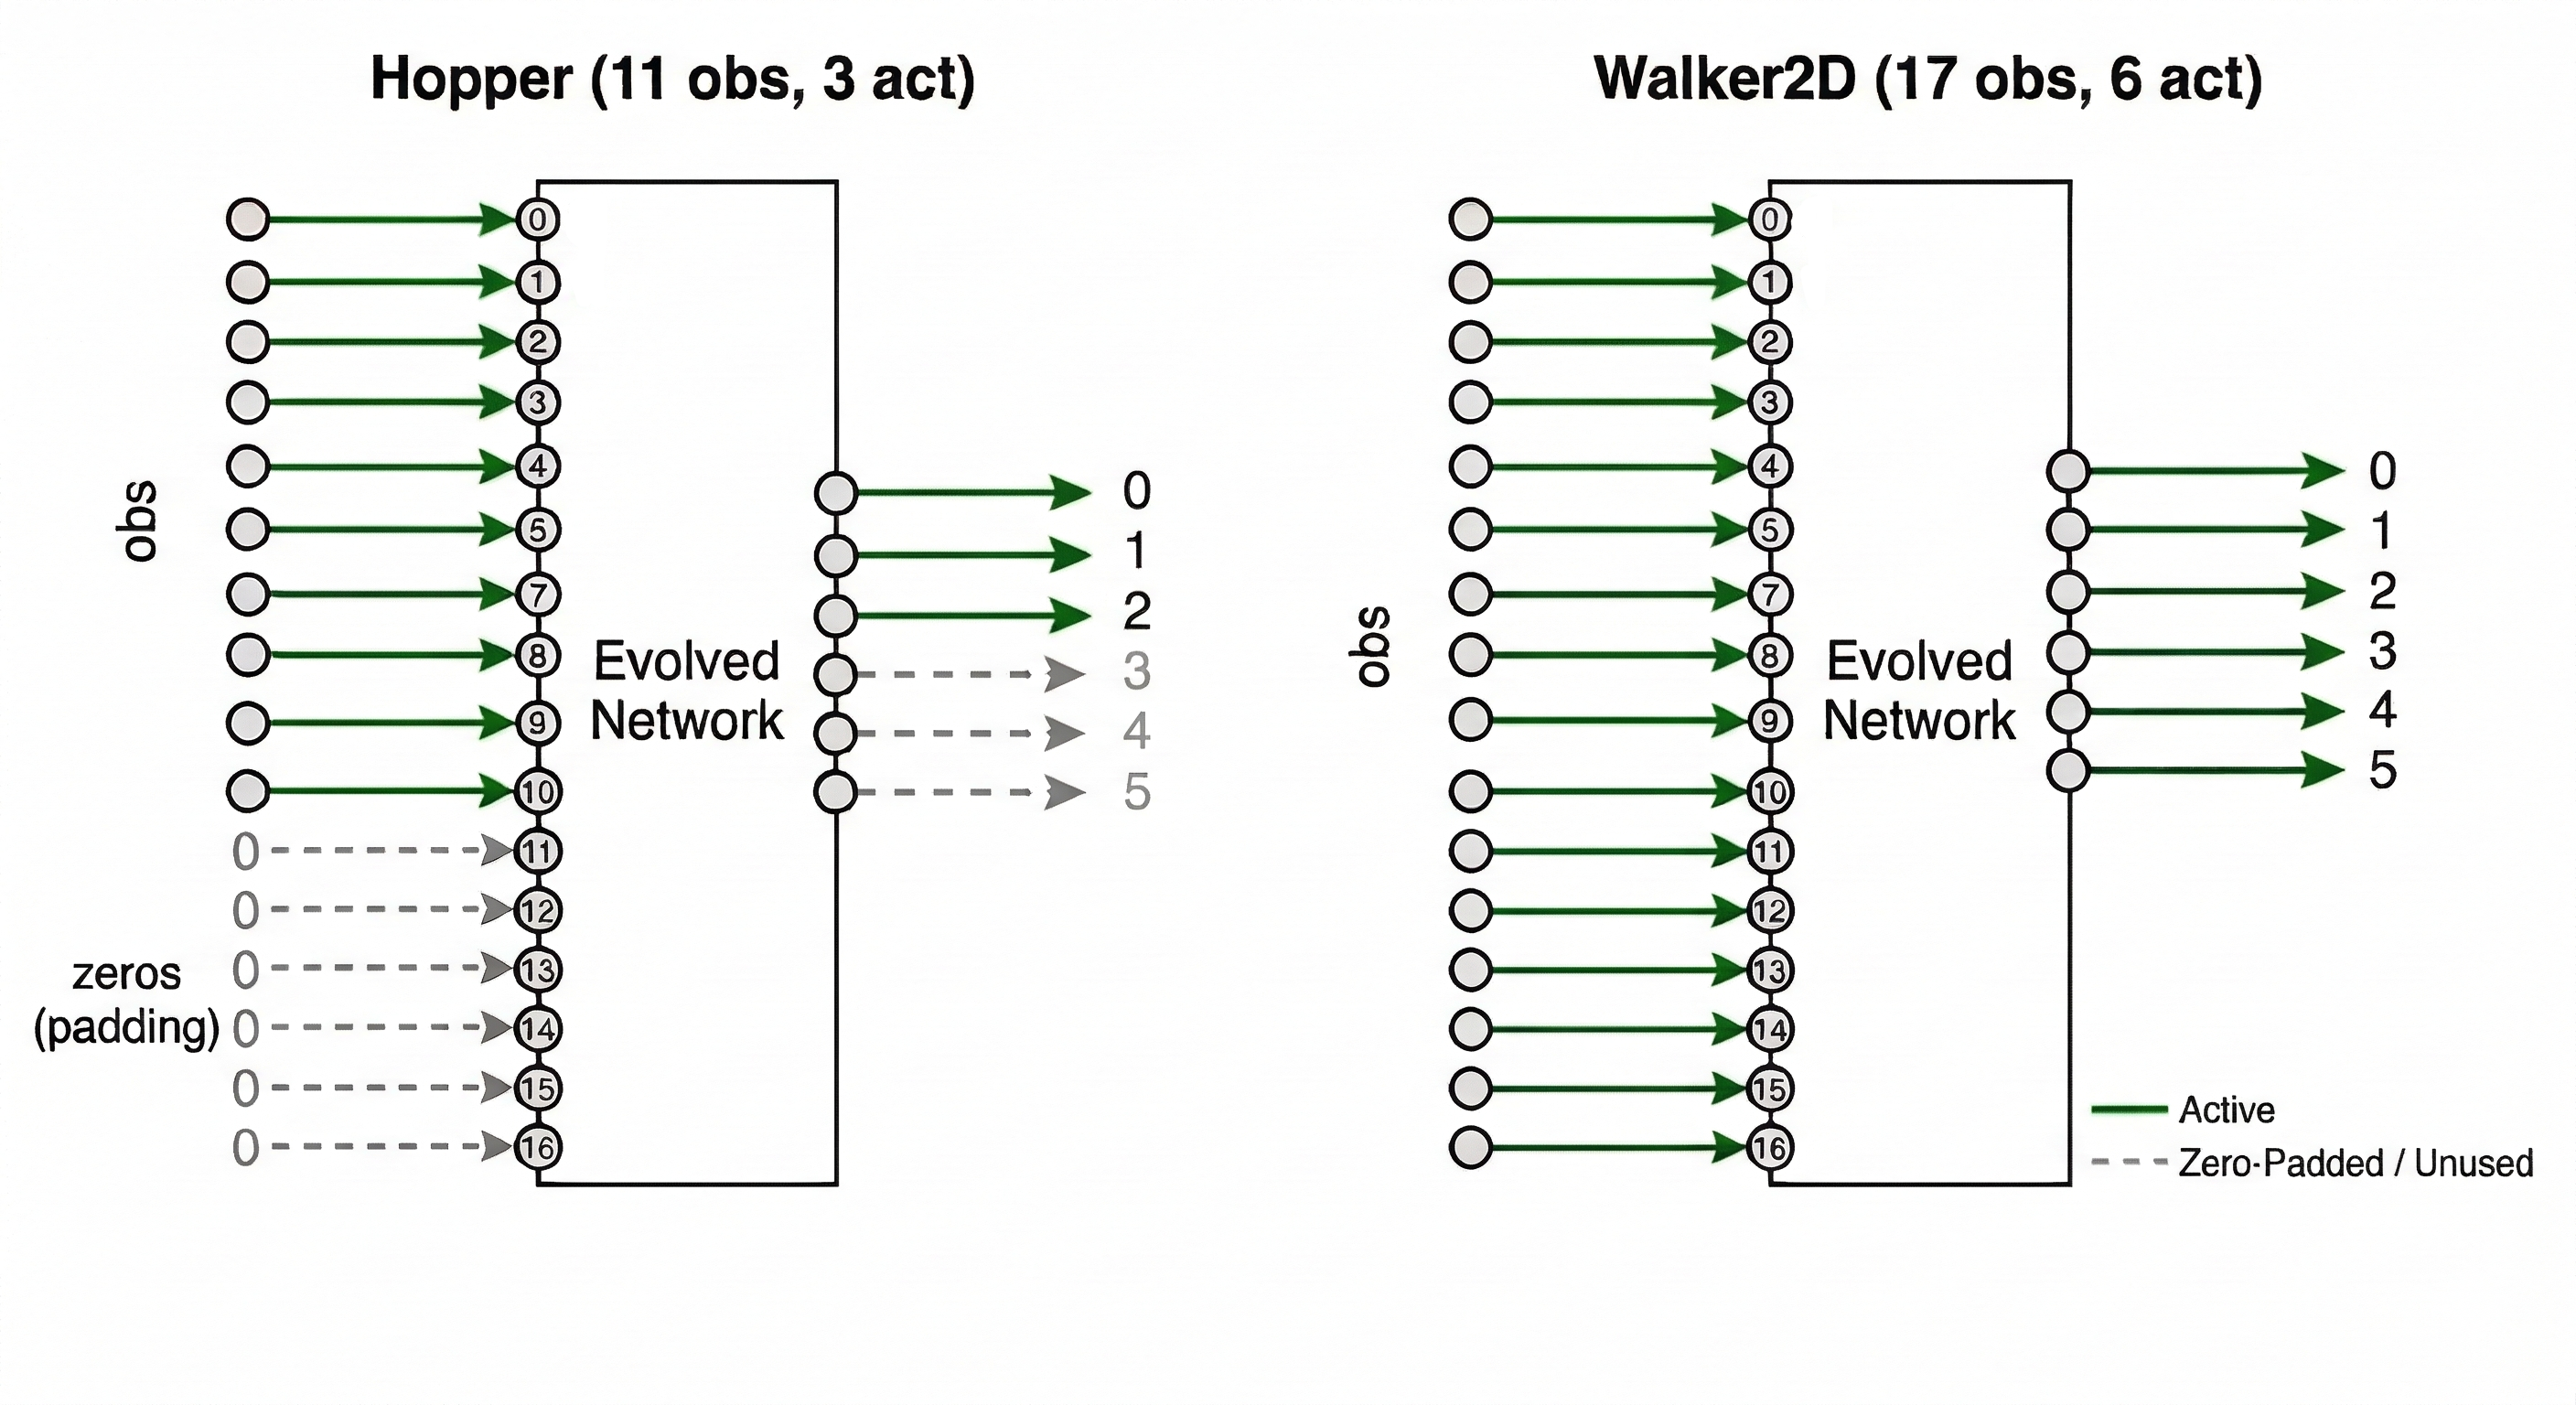
\includegraphics[width=0.85\textwidth]{Figures/Network.png}
    \caption{Network representation used in the multi-task setup.}
    \label{fig:network-architecture}
\end{figure}

The zero-padded input positions carry no reward signal from Hopper, leaving the network free to use or ignore them.
The network may learn to route Hopper-relevant computation through the first 11 input nodes while reserving the remaining 6 for Walker2D-specific processing, or it may discover shared representations spanning both input regions.
The interpretability of the padded dimensions remains an open question warranting examination in the analysis.
A rough representation of the network can be seen in Figure~\ref{fig:network-architecture}.

At the implementation level, nodes are stored as a $[N_{\max} \times 4]$ array encoding index, bias, aggregation function, and activation function per node.
Connections are stored as a $[C_{\max} \times 4]$ array encoding source index, destination index, historical marker, and weight per connection.
Inactive positions use NaN in the first column; the mask $\neg\text{isnan}(\mathbf{x}_{:,0})$ distinguishes active from inactive genes.

\subsection{Fitness Evaluation}

A critical design decision in multi-task neuroevolution is how to aggregate performance across tasks into a selection signal.
Each generation, every genome in the population is to be evaluated on both Hopper and Walker2D.
The planned evaluation pipeline proceeds in four stages:

\begin{enumerate}
    \item \textbf{Decode.} The genome's node and connection arrays are transformed into an executable network representation via topological sort and adjacency matrix construction.
    \item \textbf{Evaluate per task.} The network controls each environment for 1,000 timesteps. Each task uses an independent random key derived deterministically from the genome's evaluation key, ensuring reproducible episode generation across runs.
    \item \textbf{Normalize.} Raw fitness values are to be divided by task-specific normalisation constants to account for the differing reward scales across environments. [\textit{Normalisation constants are to be determined empirically from baseline runs.}]
    \item \textbf{Aggregate via multi-objective selection.} The normalised per-task fitnesses form a two-dimensional objective vector. Rather than collapsing these objectives into a scalar, selection is to be performed using NSGA-II (Non-dominated Sorting Genetic Algorithm II), which ranks genomes by Pareto dominance and crowding distance. This preserves the full trade-off surface between Hopper and Walker2D performance, avoiding premature convergence toward one task at the expense of the other.
\end{enumerate}

The choice of NSGA-II over scalar aggregation methods is motivated by the reward scale asymmetry between tasks.
Walker2D's reward scale substantially exceeds Hopper's, and a naive weighted sum would bias evolution toward whichever task yields larger raw returns.
Multi-objective selection sidesteps this by treating each task as an independent objective, allowing evolution to maintain a population spanning the Pareto front.

It should be noted that the NSGA-II integration is planned but not yet implemented at the time of writing.
The current prototype uses a sum of raw fitness values as an interim aggregation method.
The transition to multi-objective selection is a priority for the final experimental pipeline.

\subsection{Network Architecture}

All networks are initialised with a minimal topology: 17 input nodes connected directly to 6 output nodes, with no hidden nodes.
This follows the NEAT principle of complexification: structural complexity emerges through mutation and selection pressure rather than through designer assumptions about required network depth or width.

Output nodes apply a $\tanh$ activation to bound their values within $[-1, 1]$.
This constraint is necessary because Brax environments interpret actions as normalised joint torques: each action dimension specifies the magnitude and direction of force applied to a joint actuator, bounded to the unit interval.

Hidden nodes use per-node activation functions.
In the standard NEAT condition, all hidden nodes use $\tanh$.
In the HA-NEAT condition, the activation palette $\mathcal{A} = \{\tanh, \sigma, \text{ReLU}, \sin, \text{identity}\}$ enables heterogeneous internal representations.
The individual activation functions were selected for their complementary computational properties:

\begin{itemize}
    \item \textbf{$\tanh$) and sigmoid ($\sigma$)}: Bounded and smooth, these functions are suitable for gating behaviour and saturation dynamics, where network outputs must be constrained within a fixed range.
    \item \textbf{ReLU}: Unbounded in the positive domain, this function introduces sparsity and efficient signal propagation, properties known to be beneficial in deep network architectures.
    \item \textbf{$\sin$}: Periodic by nature, sinusoidal activation is capable of encoding oscillatory patterns, a property of particular relevance to rhythmic locomotion, where joint trajectories follow approximately periodic profiles.
    \item \textbf{Identity}: A linear pass-through that enables skip connections and linear sub-networks, allowing the evolved topology to incorporate proportional control pathways without nonlinear distortion.
\end{itemize}

The hypothesis underlying the heterogeneous palette is that a network benefits from composing these nonlinearities (periodic functions for gait timing, saturating functions for balance, and linear functions for proportional control), whereas a homogeneous $\tanh$ network must approximate all such behaviours through a single nonlinearity, potentially requiring greater structural complexity.

All hidden nodes employ sum aggregation.
That is, the pre-activation value of a node is computed as the sum of incoming weighted signals plus a bias term.
Formally, for node $j$ with incoming connections from the set of source nodes $\mathcal{I}_j$:

$$z_j = \phi_j\left(b_j + \sum_{i \in \mathcal{I}_j} w_{ij} \cdot v_i\right)$$

where $\phi_j \in \mathcal{A}$ denotes the node's activation function, $b_j$ is the bias, $w_{ij}$ are connection weights, and $v_i$ are the output values of source nodes.

\subsection{Implementation Stack}

The experiments are built upon TensorNEAT (\cite{wang_tensorized_2024}), a GPU-accelerated NEAT implementation constructed on JAX.
TensorNEAT encodes the entire evolutionary pipeline (population initialisation, mutation, crossover, speciation, fitness evaluation, and selection) as JAX-transformable functions, compiling to a single XLA computation graph via \texttt{jax.jit} executed entirely on the GPU without CPU-GPU data transfers during the evolutionary loop.
Population-level operations are vectorised using \texttt{jax.vmap}, eliminating Python-level loops over the population.
This end-to-end GPU execution was the primary motivation for selecting TensorNEAT over classical CPU-based NEAT implementations such as NEAT-Python.

Brax (\cite{freeman_brax_2021}) serves as the physics backend, implementing rigid-body simulation as differentiable JAX functions that integrate directly with TensorNEAT's JIT-compiled evaluation loop.
Brax exposes several dynamics pipelines; this work uses the \texttt{generalized} backend to keep the contact dynamics close to standard MuJoCo benchmark results reported in the reinforcement learning literature.
The combination of JAX-native evolution and JAX-native simulation eliminates the host-device transfer bottleneck that limits frameworks in which the evolutionary algorithm runs on the CPU while fitness evaluation runs on the GPU.

Experiment tracking is implemented using MLflow.
Each run logs per-generation metrics including maximum, mean, minimum, and standard deviation of fitness across the population, alongside valid genome count, generation wall-clock time, species count, stagnation counter, and the node and connection counts of the best genome.
Per-task fitness scores for the best genome are tracked separately for Hopper and Walker2D, enabling post-hoc analysis of task-specific performance trajectories and the degree to which the shared network specialises toward one environment over the other.
Fitness aggregation currently uses a raw sum of per-task rewards; a methodologically rigorous replacement using either reward normalisation or a multi-objective approach (NSGA-II) is planned for subsequent experiments.

\begin{table}[h]
\centering
\caption{MLflow Metrics Logged Per Generation}
\label{tab:mlflow_metrics}
\begin{tabular}{lll}
\toprule
\textbf{Metric} & \textbf{Description} & \textbf{Scope} \\
\midrule
\texttt{fitness/max}          & Maximum fitness in population          & Population \\
\texttt{fitness/mean}         & Mean fitness in population             & Population \\
\texttt{fitness/min}          & Minimum fitness in population          & Population \\
\texttt{fitness/std}          & Standard deviation of fitness          & Population \\
\texttt{fitness/valid\_count} & Number of successfully evaluated genomes & Population \\
\texttt{fitness/hopper}       & Best genome reward on Hopper           & Best genome \\
\texttt{fitness/walker2d}     & Best genome reward on Walker2D         & Best genome \\
\texttt{best\_fitness}        & Aggregated fitness of best genome (raw sum) & Best genome \\
\texttt{neat/n\_species}      & Number of active species               & Population \\
\texttt{stability/stagnation\_counter} & Generations without improvement & Population \\
\texttt{neat/best\_genome\_n\_nodes}  & Node count of best genome       & Best genome \\
\texttt{neat/best\_genome\_n\_conns}  & Connection count of best genome & Best genome \\
\texttt{neat/avg\_genome\_n\_conns}   & Mean connection count across population & Population \\
\texttt{cost\_time\_ms}       & Wall-clock time per generation (ms)    & Run \\
\bottomrule
\end{tabular}
\end{table}

\section{Experimental Settings}

\subsection{Environment Details}

Table 1 presents the specifications of both evaluation environments.

\begin{table}[h]
\centering
\caption{Environment Specifications}
\begin{tabular}{|l|l|l|}
\hline
\textbf{Property} & \textbf{Hopper} & \textbf{Walker2D} \\
\hline
Observation dimensions & 11 & 17 \\
\hline
Action dimensions & 3 & 6 \\
\hline
Padded input dimensions & 17 (6 zeros appended) & 17 (native) \\
\hline
Padded output dimensions & 6 (last 3 unused) & 6 (native) \\
\hline
Episode length & 1,000 timesteps & 1,000 timesteps \\
\hline
Action range & [-1, 1] (continuous) & [-1, 1] (continuous) \\
\hline
Simulator & Brax v0.14.1 (\texttt{generalized}) & Brax v0.14.1 (\texttt{generalized}) \\
\hline
\end{tabular}
\end{table}

Both environments reward forward locomotion while penalising energy expenditure and falls.
Hopper terminates an episode early if the torso height falls below a threshold or the torso tilts beyond a critical angle; Walker2D applies analogous termination conditions for its bipedal stance.
Importantly, the reward structures differ in scale: Walker2D typically yields higher cumulative rewards than Hopper for equivalent locomotion quality.
This scale asymmetry is a primary motivation for the normalisation and multi-objective selection approach described in the Fitness Evaluation section.

\subsection{Hyperparameters}

Table 2 lists the evolutionary hyperparameters used across both experimental conditions.
Values marked with [*] are placeholders pending determination through preliminary calibration runs.

\begin{table}[h]
\centering
\caption{Evolutionary Hyperparameters}
\begin{tabular}{|l|l|}
\hline
\textbf{Parameter} & \textbf{Value} \\
\hline
Population size & [*TBD*] \\
\hline
Generation limit & [*TBD*] \\
\hline
Fitness target & [*TBD*] \\
\hline
Max nodes per genome & [*TBD*] \\
\hline
Max connections per genome & [*TBD*] \\
\hline
Target species count & [*TBD*] \\
\hline
Compatibility threshold ($\theta$) & 1.0 \\
\hline
Survival threshold & 0.1 \\
\hline
Max species stagnation & 15 \\
\hline
Species elitism & 2 \\
\hline
Genome elitism & 2 \\
\hline
Connection add probability & 0.2 \\
\hline
Connection delete probability & 0.2 \\
\hline
Node add probability & 0.1 \\
\hline
Node delete probability & 0.1 \\
\hline
Bias init mean / std & 0.0 / 1.0 \\
\hline
Bias mutate power / rate & 0.15 / 0.2 \\
\hline
Bias replace rate & 0.015 \\
\hline
Weight init mean / std & 0.0 / 1.0 \\
\hline
Weight mutate power / rate & 0.5 / 0.8 \\
\hline
Weight replace rate & 0.1 \\
\hline
\textbf{HA-NEAT specific} & \\
\hline
Activation mutation rate ($p_{\text{act}}$) & 0.1 \\
\hline
Activation palette & $\{\tanh, \sigma, \text{ReLU}, \sin, \text{identity}\}$ \\
\hline
Standard activation replace rate & 0.0 (disabled) \\
\hline
Historical marker reassignment & Enabled (via OriginConn) \\
\hline
\end{tabular}
\end{table}

The compatibility threshold $\theta = 1.0$ and survival threshold of 0.1 follow standard NEAT practice as established in the original NEAT literature.
The survival threshold dictates that only the top 10\% of each species produces offspring, creating strong within-species selection pressure while speciation protects structural diversity across the population as a whole.

\subsection{Experimental Conditions}

The experiment compares two conditions, both operating within the multi-task Hopper + Walker2D setting:

\begin{enumerate}
    \item \textbf{Multi-Task NEAT (baseline).} Standard NEAT with homogeneous $\tanh$ activation functions on all hidden nodes. This condition uses \texttt{DefaultConn} without historical markers. The standard per-node activation mutation mechanism is active but has no practical effect, since only one activation option is available.
    
    \item \textbf{Multi-Task HA-NEAT (treatment).} HA-NEAT with heterogeneous activations drawn from the palette $\mathcal{A}$. This condition uses \texttt{OriginConn} with historical markers. Activation mutation occurs at most once per genome per generation, with speciation protection via marker reassignment as described in Section \textit{HA-NEAT Extensions}.
\end{enumerate}

Both conditions use identical population sizes, generation limits, structural mutation rates, and evaluation procedures.
The independent variable is the activation function regime: homogeneous activations versus heterogeneous activations with speciation protection.
The dependent variables are:

\begin{itemize}
    \item \textbf{Per-task fitness}: Best and mean fitness on Hopper and Walker2D individually, measured per generation.
    \item \textbf{Combined Pareto front quality}: Hypervolume of the Pareto front in the (Hopper fitness, Walker2D fitness) objective space, quantifying the breadth and quality of multi-task trade-off solutions.
    \item \textbf{Genome complexity}: Number of active nodes and connections in the best genome per generation, measuring the structural cost of evolved solutions.
    \item \textbf{Species dynamics}: Number of active species per generation, serving as a proxy for population diversity.
\end{itemize}

\subsection{Evaluation Protocol}

Each experimental condition is to be repeated across a minimum of 10 independent runs with different random seeds.
This sample size is chosen to provide sufficient statistical power for detecting medium-to-large effect sizes with non-parametric tests, while remaining computationally tractable given the cost of large-population neuroevolution on GPU hardware.

Performance is measured at three levels:

\begin{enumerate}
    \item \textbf{Per-generation tracking.} Every generation, the pipeline logs maximum, mean, minimum, and standard deviation of population fitness; per-task fitness of the best genome; species count; and best-genome node and connection counts.
    \item \textbf{Final performance.} The best fitness achieved across all generations per run, reported as median and interquartile range across the 10+ independent runs.
    \item \textbf{Learning dynamics.} Fitness-over-generation curves, averaged across runs with 95\% confidence bands, to characterise convergence speed and stability.
\end{enumerate}

Statistical comparison between the NEAT baseline and HA-NEAT treatment uses the Mann-Whitney U test (two-sided, $\alpha = 0.05$) applied to the distribution of best fitnesses across runs.
This non-parametric test is appropriate because evolutionary run outcomes are not guaranteed to follow a normal distribution, and the moderate sample size does not reliably support parametric assumptions.

\subsection{Compute Resources}

All experiments are conducted on a single compute node with the specifications listed in Table 3.

\begin{table}[h]
\centering
\caption{Compute Node Specifications}
\begin{tabular}{|l|l|}
\hline
\textbf{Component} & \textbf{Specification} \\
\hline
CPU & AMD Threadripper 7970X (32 cores, 64 threads) \\
\hline
RAM & 251 GB \\
\hline
GPU & 2$\times$ NVIDIA RTX A6000 (49 GB VRAM each) \\
\hline
CUDA & 12.4 \\
\hline
Software & JAX [*version TBD*], Brax 0.14.1, Python 3.10+ \\
\hline
\end{tabular}
\end{table}

Each evolutionary run utilises a single GPU.
The dual-GPU configuration enables two independent runs to execute in parallel, halving the wall-clock time required for the full experimental campaign.
JIT compilation of the evolutionary step occurs once at the start of each run; subsequent generations execute the compiled XLA graph without recompilation overhead, with the exception of topology-triggered recompilation events that occur when the population's maximum genome size changes.

%\section{Background}

% \section{Methodology}

% \subsection{Problem Formulation}


% The pairing of Hopper and Walker2D is deliberate: both are planar locomotion domains with related lower-limb mechanics, but different body complexity and control demands. Hopper can be interpreted as a constrained single-leg locomotor, whereas Walker2D requires coordinated bilateral stepping. This creates a useful transfer setting: structural regularities (e.g., balance, forward propulsion, leg extension/flexion timing) can be shared, while increased task complexity still demands specialization. The central hypothesis is that HA-NEAT can discover shared substructures and task-specific neuronal roles without manually engineered modularization.

% \subsection{Algorithm Design (HA-NEAT)}
% The method builds on canonical NEAT by evolving not only topology and connection weights, but also neuron-level activation functions (heterogeneous activation NEAT, HA-NEAT). Each genome contains:
% \begin{itemize}
%     \item node genes (node id, type, activation-function id),
%     \item connection genes (in-node, out-node, weight, enabled flag, innovation id).
% \end{itemize}

% Compared to vanilla NEAT, the key extension is an \textit{activation mutation} operator that can change a hidden node's activation function from a predefined library (e.g., ReLU, Tanh, Sigmoid, Gaussian, Sine, Identity). This allows local nonlinearities to co-evolve with topology.

% To support cross-environment evaluation with one genotype, all networks use a unified I/O interface. Inputs are padded to 28 dimensions and outputs to 9 dimensions. For each environment, only task-valid features and actuators are populated; all non-applicable entries are set to zero (zero-masking). Concretely, a Hopper observation/action pair is embedded into the 28/9 vector with deterministic index mapping, and Walker2D uses the same global index system. During rollout, invalid action channels are masked out before being passed to the simulator. This preserves one genome space while allowing task-specific sparsity.

% Mutation and crossover follow NEAT principles with innovation tracking for homologous alignment. Structural mutations include add-node and add-connection; parametric mutations perturb weights; activation mutations alter local transfer functions. Crossover combines matching genes by innovation number and inherits disjoint/excess genes under the configured fitness-parent rule. Speciation uses compatibility distance over structural and parametric differences to protect innovation and prevent immediate elimination of novel topologies.

% \subsection{Fitness Evaluation}
% Each candidate genome is evaluated in both environments within the same generation. Let $R_{\text{H}}$ and $R_{\text{W}}$ denote episode returns (or mean returns over repeated evaluation episodes) for Hopper and Walker2D. To make scales comparable, rewards are normalized by environment-specific solved thresholds $\tau_{\text{H}}$ and $\tau_{\text{W}}$:
% \[
% \hat{R}_{\text{H}}=\frac{R_{\text{H}}}{\tau_{\text{H}}},\qquad
% \hat{R}_{\text{W}}=\frac{R_{\text{W}}}{\tau_{\text{W}}}.
% \]
% The primary scalar fitness is then
% \[
% F=\frac{\hat{R}_{\text{H}}+\hat{R}_{\text{W}}}{2},
% \]
% which equally weights both tasks and discourages specialization to only one environment.

% This aggregation yields a standard single-objective evolutionary loop while still reflecting balanced multi-task competence. As an extension, the same pipeline can be converted into a Pareto formulation with objectives $(\hat{R}_{\text{H}},\hat{R}_{\text{W}})$ and optimized using NSGA-II to explicitly trace trade-offs between task-specific and joint performance.

% \subsection{Network Architecture}
% The phenotype network is represented through a padded graph view that is compatible with a fixed-size adjacency-matrix implementation. At initialization, $\texttt{init\_hidden\_layers=()}$ creates a minimal topology: direct input-to-output connectivity in NEAT style, no hidden layer prior, and random initial weights. This biases search toward simple policies first.

% Complexification then grows topology over generations by selectively inserting new hidden nodes and edges. Insertion of a node splits an existing edge, preserving functional continuity while increasing representational capacity. Add-connection mutations create shortcuts or recurrently useful pathways (if recurrence is enabled by configuration). Because hidden nodes also carry activation-function genes, structural growth and nonlinear diversification are coupled: new subnetworks can emerge with distinct inductive biases for different control motifs (e.g., near-linear stabilization vs.
% nonlinear gait timing).

% Under the padded 28-input/9-output interface, the adjacency representation remains constant in shape across tasks, while the active computational subgraph differs via masking. This allows one evolving topology to host both shared pathways and sparse, task-specific branches.

% \subsection{Implementation Stack}
% The implementation uses TensorNEAT on top of JAX, with Brax as the physics backend. This stack is selected for efficient batched neuroevolution in continuous control. JAX enables vectorized population evaluation and just-in-time (JIT) compilation of rollout and fitness code paths. Brax provides differentiable, accelerator-friendly rigid-body simulation and integrates naturally with JAX tensors.

% The practical advantage is reduced host-device overhead: policy execution, simulation stepping, and fitness aggregation can run in a compiled on-device pipeline rather than frequent CPU--GPU synchronization. For evolutionary methods that evaluate many genomes per generation, this substantially improves throughput and makes repeated multi-run experiments tractable.

% \section{Experimental settings}

% \subsection{Environment Details}
% Table~\ref{tab:env-details} summarizes the two tasks used in this thesis. Both are episodic continuous-control locomotion benchmarks with forward-progress rewards and instability-based terminations.

% \begin{table}[h]
% \centering
% \caption{Environment configuration used for multi-task training and evaluation.}
% \label{tab:env-details}
% \begin{tabular}{lcc}
% \hline
% Property & Hopper & Walker2D \\
% \hline
% Observation dimension & 11 & 17 \\
% Action dimension & 3 & 6 \\
% Padded input dimension & 28 & 28 \\
% Padded output dimension & 9 & 9 \\
% Primary reward signal & Forward locomotion & Forward locomotion \\
% Episode length (max steps) & 1000 & 1000 \\
% Termination & Fall/instability or timeout & Fall/instability or timeout \\
% \hline
% \end{tabular}
% \end{table}

% \subsection{Hyperparameters}
% All evolutionary hyperparameters are fixed across conditions unless explicitly stated otherwise. Table~\ref{tab:hyperparams} lists the core settings.

% \begin{table}[h]
% \centering
% \caption{Core HA-NEAT hyperparameters.}
% \label{tab:hyperparams}
% \begin{tabular}{ll}
% \hline
% Hyperparameter & Value \\
% \hline
% Population size & 512 \\
% Number of generations & 300 \\
% Compatibility threshold $\delta_t$ & 3.0 \\
% Species target & 15 \\
% Crossover rate & 0.75 \\
% Weight mutation rate & 0.80 \\
% Add-node mutation rate & 0.03 \\
% Add-connection mutation rate & 0.05 \\
% Activation mutation rate & 0.10 \\
% Elitism (per species) & 1 \\
% Stagnation limit & 20 generations \\
% \hline
% \end{tabular}
% \end{table}

% \subsection{Experimental Conditions / Independent Variables}
% The primary independent variable is activation-function heterogeneity. We compare:
% \begin{itemize}
%     \item \textbf{Homogeneous baseline}: all hidden nodes use one fixed activation function (ReLU),
%     \item \textbf{Heterogeneous HA-NEAT}: hidden nodes evolve activation type from a shared library.
% \end{itemize}

% The activation-function library for heterogeneous conditions consists of ReLU, Tanh, Sigmoid, Gaussian, Sine, and Identity. This set mixes saturating and non-saturating nonlinearities, localized and periodic responses, and a linear passthrough option. A secondary condition compares \textit{single-task} evolution (Hopper-only or Walker2D-only fitness) against \textit{multi-task} evolution (joint normalized fitness), to isolate transfer effects.

% \subsection{Evaluation Protocol}
% Each condition is executed with multiple random seeds to quantify stochastic variability. The target protocol is 10 independent runs per condition (minimum acceptable: 5). For each run, we log best-genome fitness per generation, population mean fitness, species count, and topology size statistics (nodes/connections).

% Performance is reported on normalized task return and joint fitness. A run is marked as solved for a task when its best genome reaches or exceeds the corresponding solved threshold. Between-condition comparisons use non-parametric tests (Mann--Whitney U for pairwise comparisons) with effect size reporting (Cliff's $\delta$), and Holm correction when multiple pairwise tests are performed.

% \subsection{Compute Resources}
% All experiments are executed on NOVA DAH 01 equipped with an NVIDIA RTX A6000 GPU (48 GB VRAM). The software stack uses CUDA 12.x with JAX-compatible acceleration. Reporting hardware and CUDA runtime is necessary because population-level JIT execution and simulator throughput are sensitive to device class and driver/runtime compatibility.
\newpage

\section{Results and Discussion}

\subsection{Experimental overview}
We trained NEAT and HA-NEAT on the same multi-task problem: a single evolved network must control both Hopper (11 observations, 3 actions) and Walker2D (17 observations, 6 actions).
The network is sized to the larger task.
Hopper observations are zero-padded to 17 dimensions, and the 6-dimensional output is sliced to 3 for Hopper's actuators.
Fitness is the normalized minimum across both tasks, ethat is, the worse of the two normalized per-task rewards.
A network that learns Hopper well but neglects Walker2D scores poorly.
That matters: a genome that gets good at Hopper while ignoring Walker2D will score on Walker2D, the task it neglected.
The aggregation selection study (Methodology, Section 3) landed on this after normalized-sum and normalized-product both let genomes specialize their way to a decent aggregate score.
\\comm

We trained NEAT and HA-NEAT on the same multi-task problem: a single evolved network must control both Hopper (11 observations, 3 actions) and Walker2D (17 observations, 6 actions). using the same weights.
The network is sized to Walker2D; Hopper observations are zero-padded to 17 dimensions, and the 6-dimensional output is sliced down to 3 for Hopper's actuators.
Fitness is the normalized minimum of the two per-task scores.
That matters: a genome that gets good at Hopper while ignoring Walker2D will score on Walker2D, the task it neglected.
The aggregation selection study \todo{Link to methodology section here}(Methodology, Section 3) landed on this after normalized-sum and normalized-product both let genomes specialize their way to a decent aggregate score.

The chapter works through the results in layers of the primary experiment head-to-head, per-task breakdowns, a re-evaluation of whether training-time fitness holds up across multiple episodes, species and complexity dynamics, and the ablation study on activation diversity.

Three experiments make up the comparison.
First, the main head-to-head: NEAT vs.\ HA-NEAT across population sizes, generation counts, and random seeds.
Second, a multi-episode re-evaluation of saved genomes, because training fitness comes from a single episode and may not reflect actual policy quality.
Third, an ablation that runs HA-NEAT's full machinery with a single activation function, testing whether any advantage comes from activation diversity or from the structural changes around it.
Section 5.2 reports aggregate performance, Section 5.3 breaks it down per task, Section 5.4 compares training estimates to re-evaluation, Section 5.5 covers species dynamics and genome complexity, and Section 5.6 presents the ablation.

All runs used the MJX (MuJoCo on GPU) physics backend, population sizes of 1024--4096, and between 500 and 2000 generations. [PLACEHOLDER: final hardware details, GPU type, JIT compile time, wall-clock per generation].
Random seeds were drawn from $\{42, 123, 75, 7, 21\}$; preliminary results use subsets of 2--3 seeds, and the final experiment uses all 5.

\subsection{Ablation: activation diversity vs.\ HA-NEAT machinery}
HA-NEAT changes two things relative to standard NEAT.
First, it draws per-node activations from a set of five functions (tanh, sigmoid, relu, sin, identity) instead of a single fixed one.
Second, it uses OriginConn, a connection gene that tracks historical innovation markers.
When a node's activation is mutated, all connections touching that node receive new markers, which increases the genetic distance between the mutant and its parent.
This pushes the mutant into a separate species, shielding it from crossover with genomes that still use the old activation.

The performance difference in Section 5.2 could come from either change, or from their interaction.
To isolate the two, we ran an ablation that keeps the full HA-NEAT machinery (OriginConn, HANEATMutation, marker reassignment) but restricts it to a single activation function (tanh).
The activation mutation still fires, but since there is only one option, nothing actually changes.
This gives us HA-NEAT's structural changes without the diversity.

\subsubsection{Training performance}

\begin{table}[h]
\centering
\caption{Ablation training results: aggregate normalized-minimum fitness. Pop$=1024$, 500 generations, 3 seeds. HA-NEAT ablation uses HA-NEAT infrastructure with tanh only.}
\label{tab:ablation-training-results}
\begin{tabular}{lcccc}
\toprule
Method & Seed 42 & Seed 75 & Seed 123 & Mean \\
\midrule
NEAT & 0.414 & 0.342 & 0.381 & 0.379 \\
HA-NEAT ablation (tanh only) & 0.352 & 0.342 & 0.398 & 0.364 \\
\bottomrule
\end{tabular}
\end{table}

\begin{figure}[h]
\centering
\begin{minipage}[t]{0.49\textwidth}
\centering
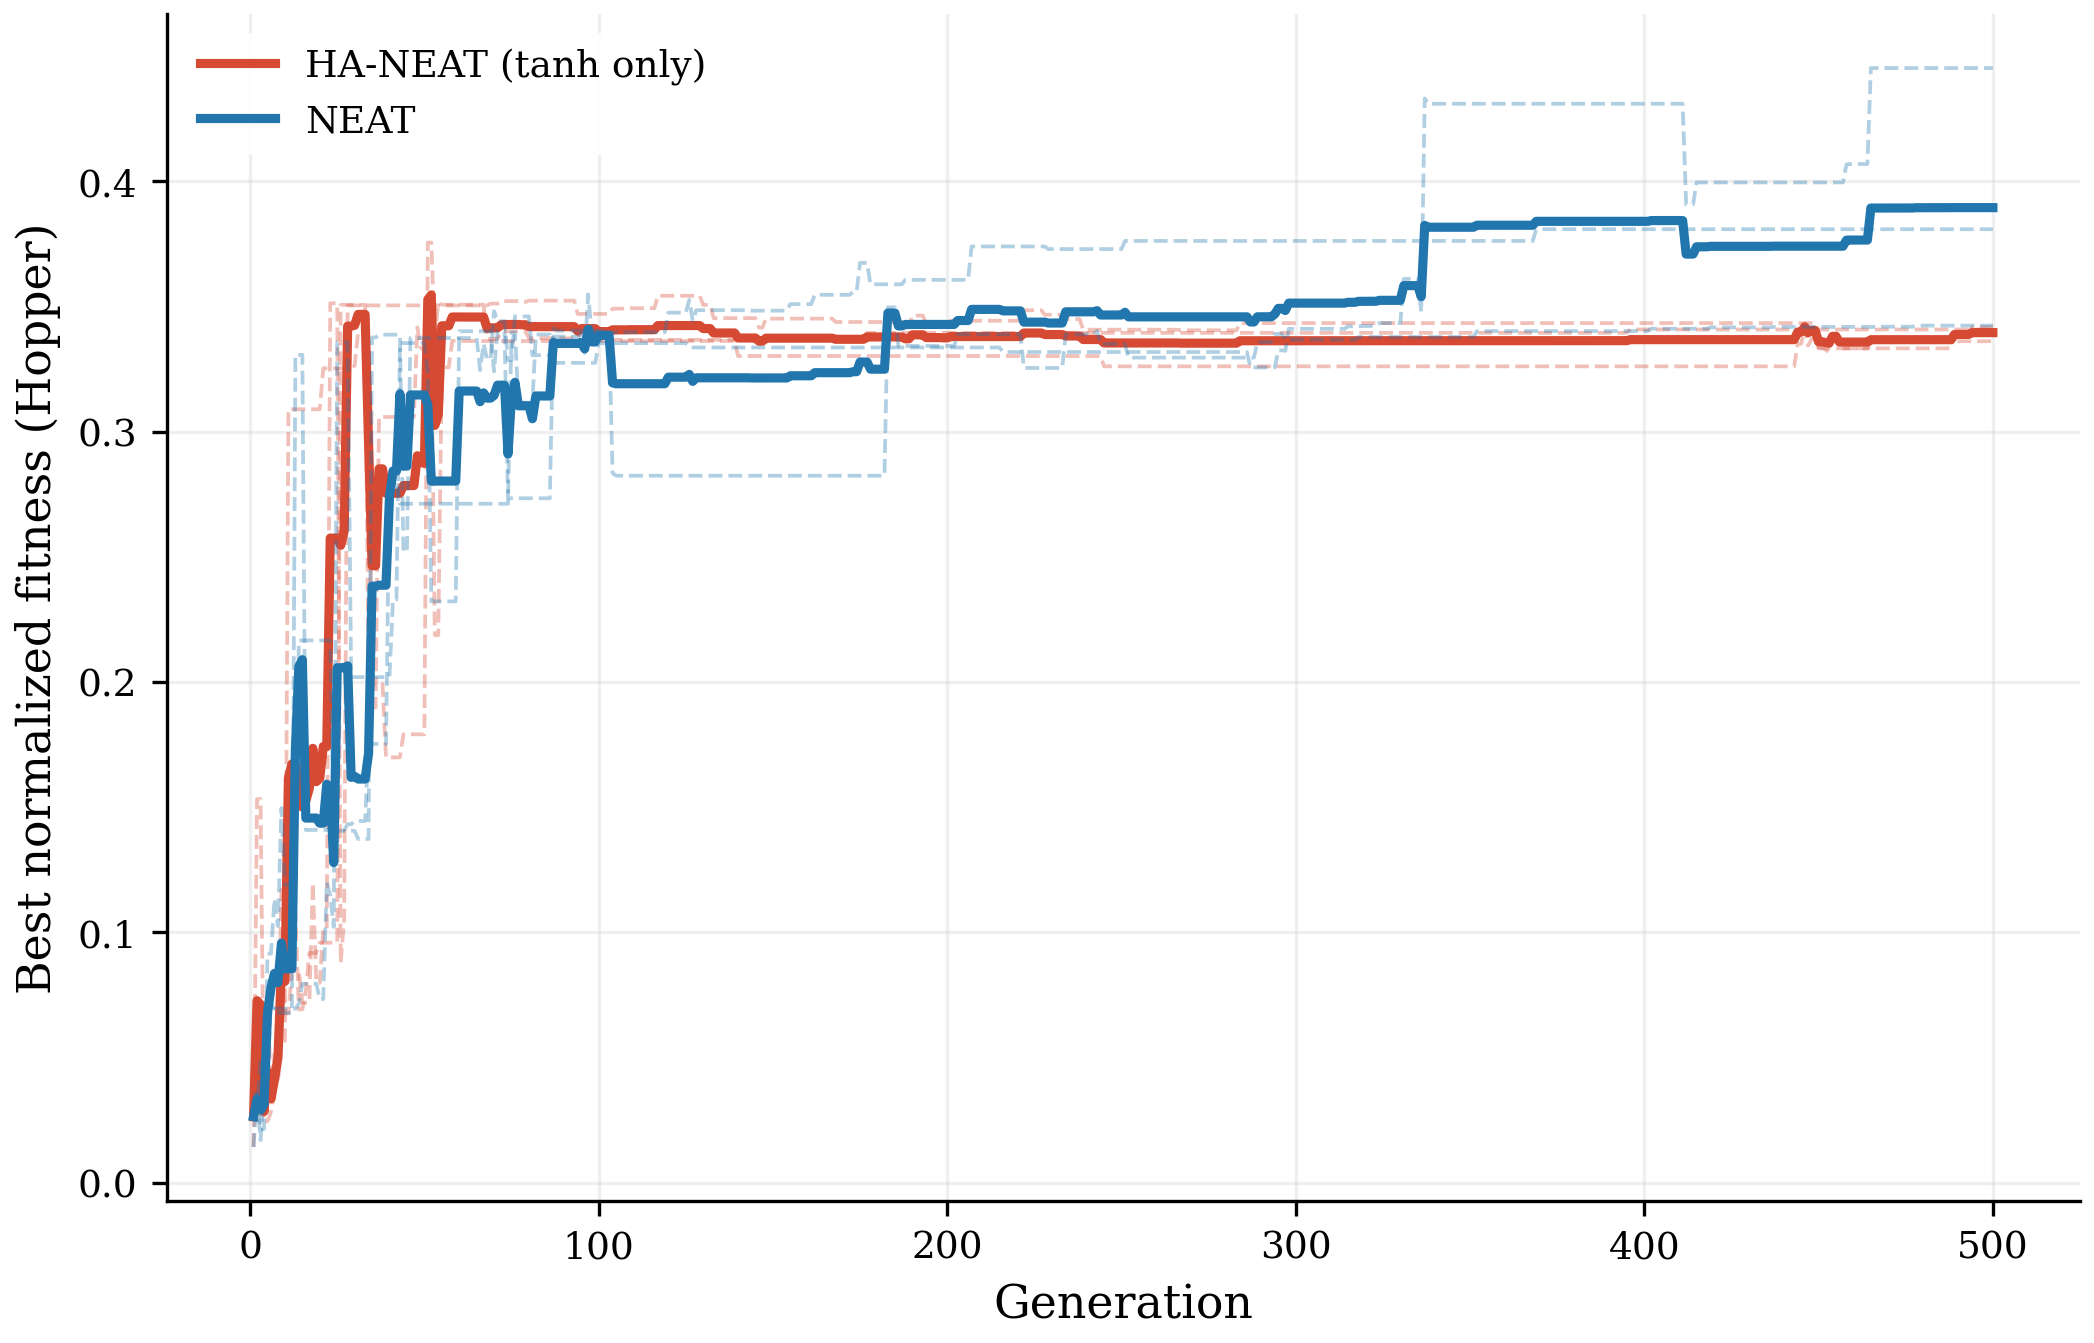
\includegraphics[width=\textwidth]{Figures/multi_task_neat_vs_haneat_ablation_training_hopper.png}
\textit{(a) Hopper best normalized fitness over 500 generations.}
\end{minipage}\hfill
\begin{minipage}[t]{0.49\textwidth}
\centering
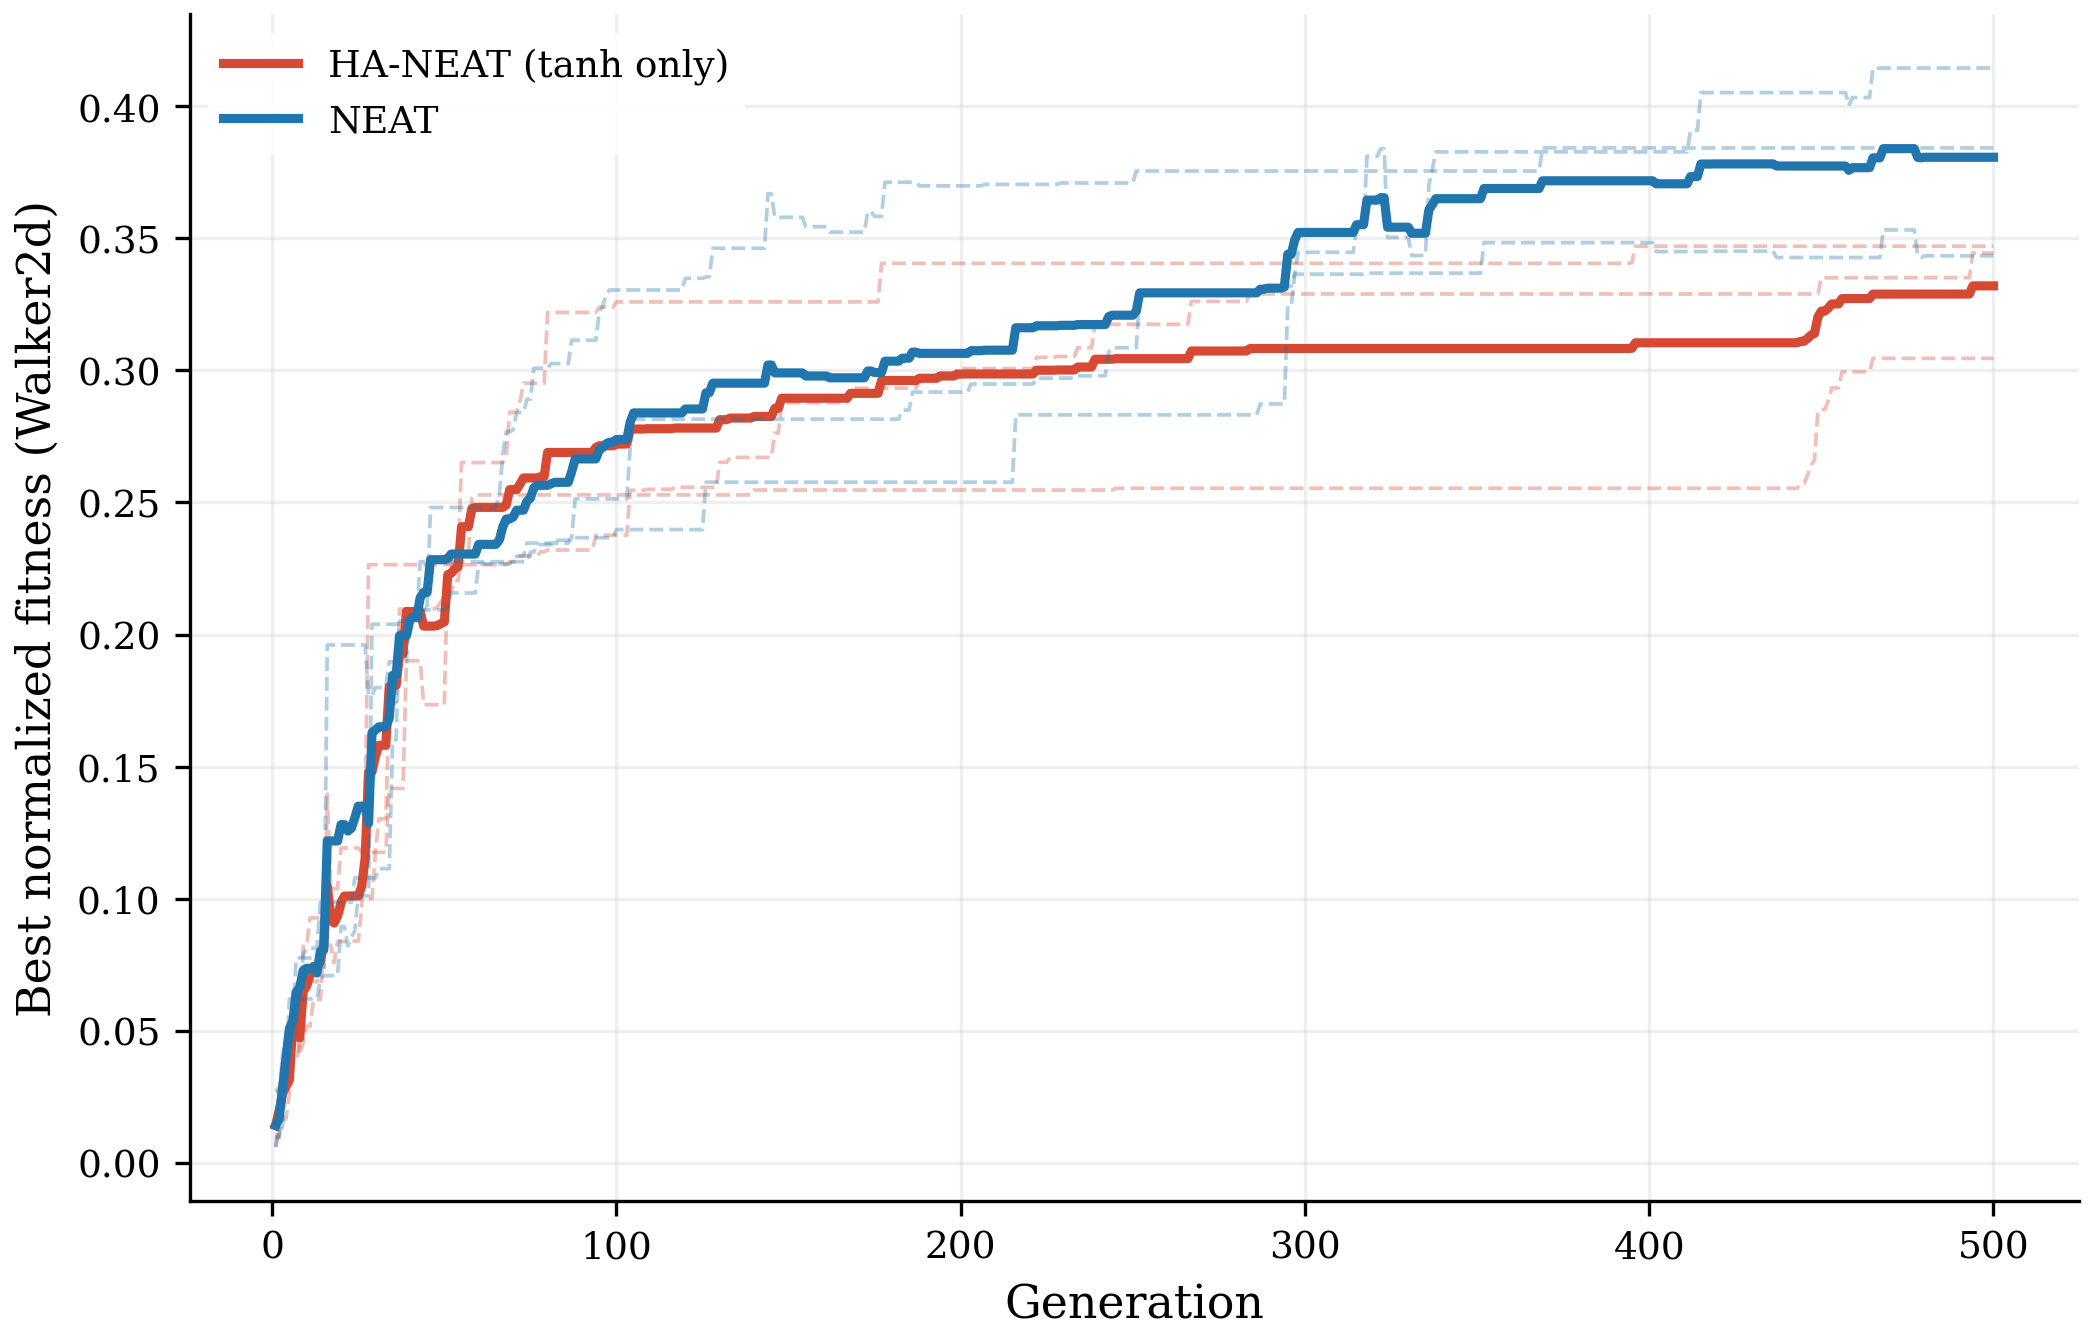
\includegraphics[width=\textwidth]{Figures/multi_task_neat_vs_haneat_ablation_training_walker2d.png}
\textit{(b) Walker2D best normalized fitness over 500 generations.}
\end{minipage}
\caption{Training curves for the ablation experiment on the two individual environments. Individual seed traces are shown with low opacity, and bold lines indicate means across seeds.}
\label{fig:ablation-training-envs}
\end{figure}

\begin{figure}[h]
\centering
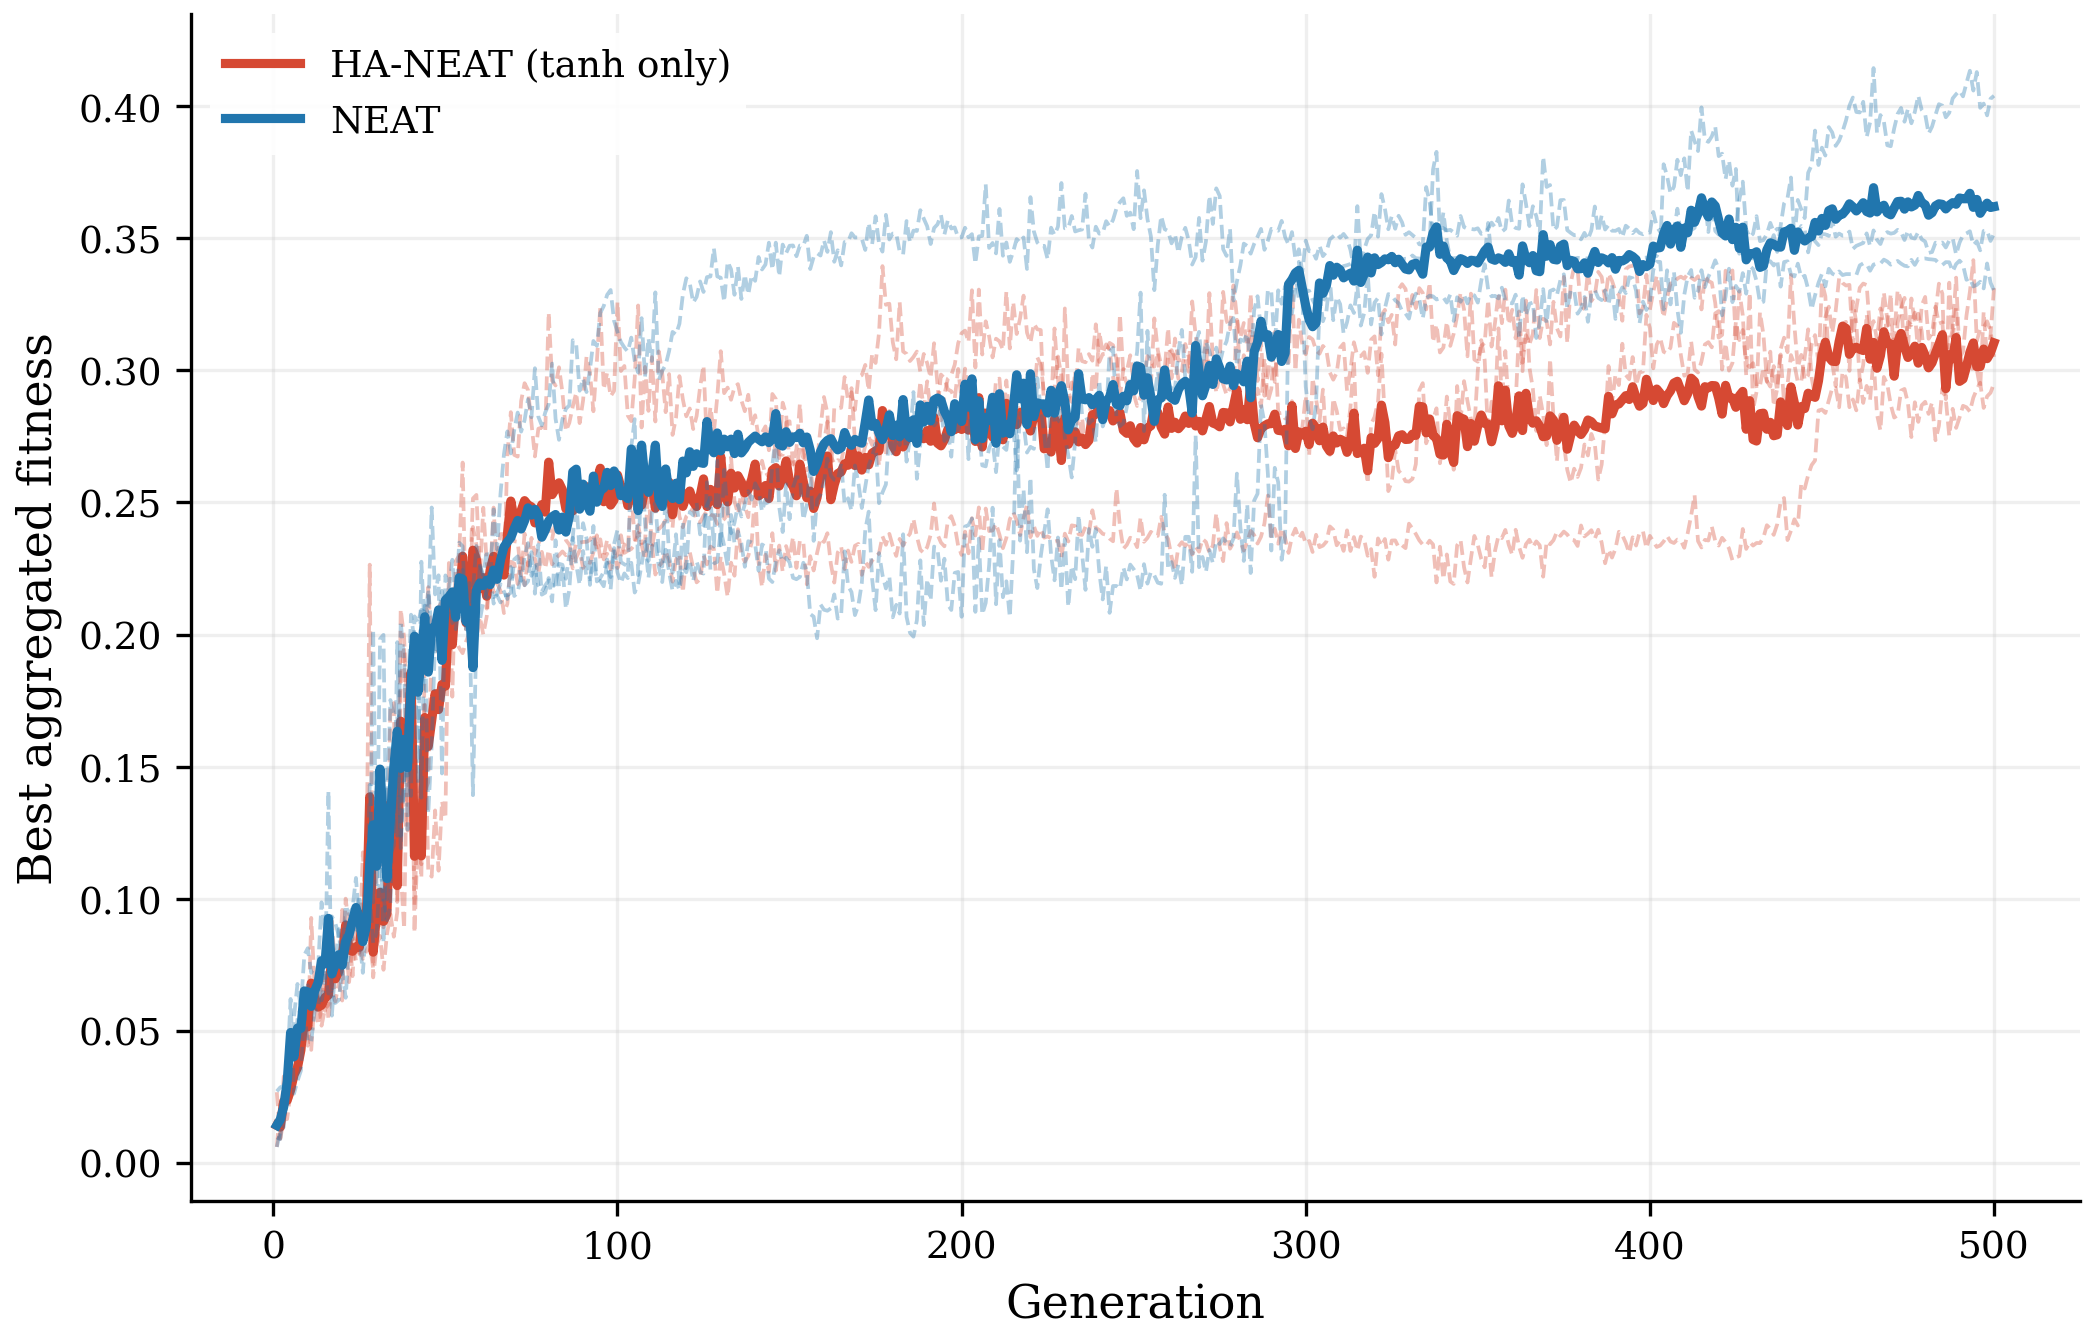
\includegraphics[width=0.8\textwidth]{Figures/multi_task_neat_vs_haneat_ablation_training_aggregated.png}
\caption{Aggregated normalized-minimum training curve for the ablation experiment. Individual seed traces are shown with low opacity, and bold lines indicate means across seeds.}
\label{fig:ablation-training-agg}
\FloatBarrier
\end{figure}


The ablation averaged 0.364 across three seeds, slightly below NEAT's 0.379.
Figures~\ref{fig:ablation-training-envs} and~\ref{fig:ablation-training-agg} are more informative than the endpoint.
On Hopper, both methods converge to similar levels with NEAT around 0.39 and HA-NEAT 0.34.
Walker2D is where they diverge: NEAT pulls ahead after around generation 150 and ends at 0.40 compared to the ablation's $\approx 0.33$.
The aggregated fitness reflects that Walker2D gap, with NEAT at $\approx 0.36$ and the ablation at $\approx 0.31$ by generation 500.

\subsubsection{Re-evaluation}

Training fitness comes from a single episode per genome, so we re-evaluated each of the six saved genomes over 30 episodes with different random seeds.
Table~\ref{tab:ablation-reeval-results} reports the results.

\begin{table}[h]
\centering
\caption{Ablation re-evaluation results: mean reward over 30 episodes per genome, 3 seeds per method. Aggregate is the normalized minimum across both tasks, computed per seed and then averaged.}
\label{tab:ablation-reeval-results}
\resizebox{\textwidth}{!}{%
\begin{tabular}{lccccc}
\toprule
Method & \shortstack{Hopper\\(mean $\pm$ std)} & \shortstack{Hopper\\(norm)} & \shortstack{Walker2D\\(mean $\pm$ std)} & \shortstack{Walker2D\\(norm)} & \shortstack{Aggregated\\(norm min)} \\
\midrule
NEAT & $1059 \pm 52$ & $0.353 \pm 0.017$ & $1288 \pm 635$ & $0.258 \pm 0.127$ & $0.241 \pm 0.101$ \\
HA-NEAT ablation & $1083 \pm 76$ & $0.361 \pm 0.025$ & $1449 \pm 533$ & $0.290 \pm 0.107$ & $0.287 \pm 0.101$ \\
\bottomrule
\end{tabular}%
}
\end{table}

\begin{figure}[h]
\centering
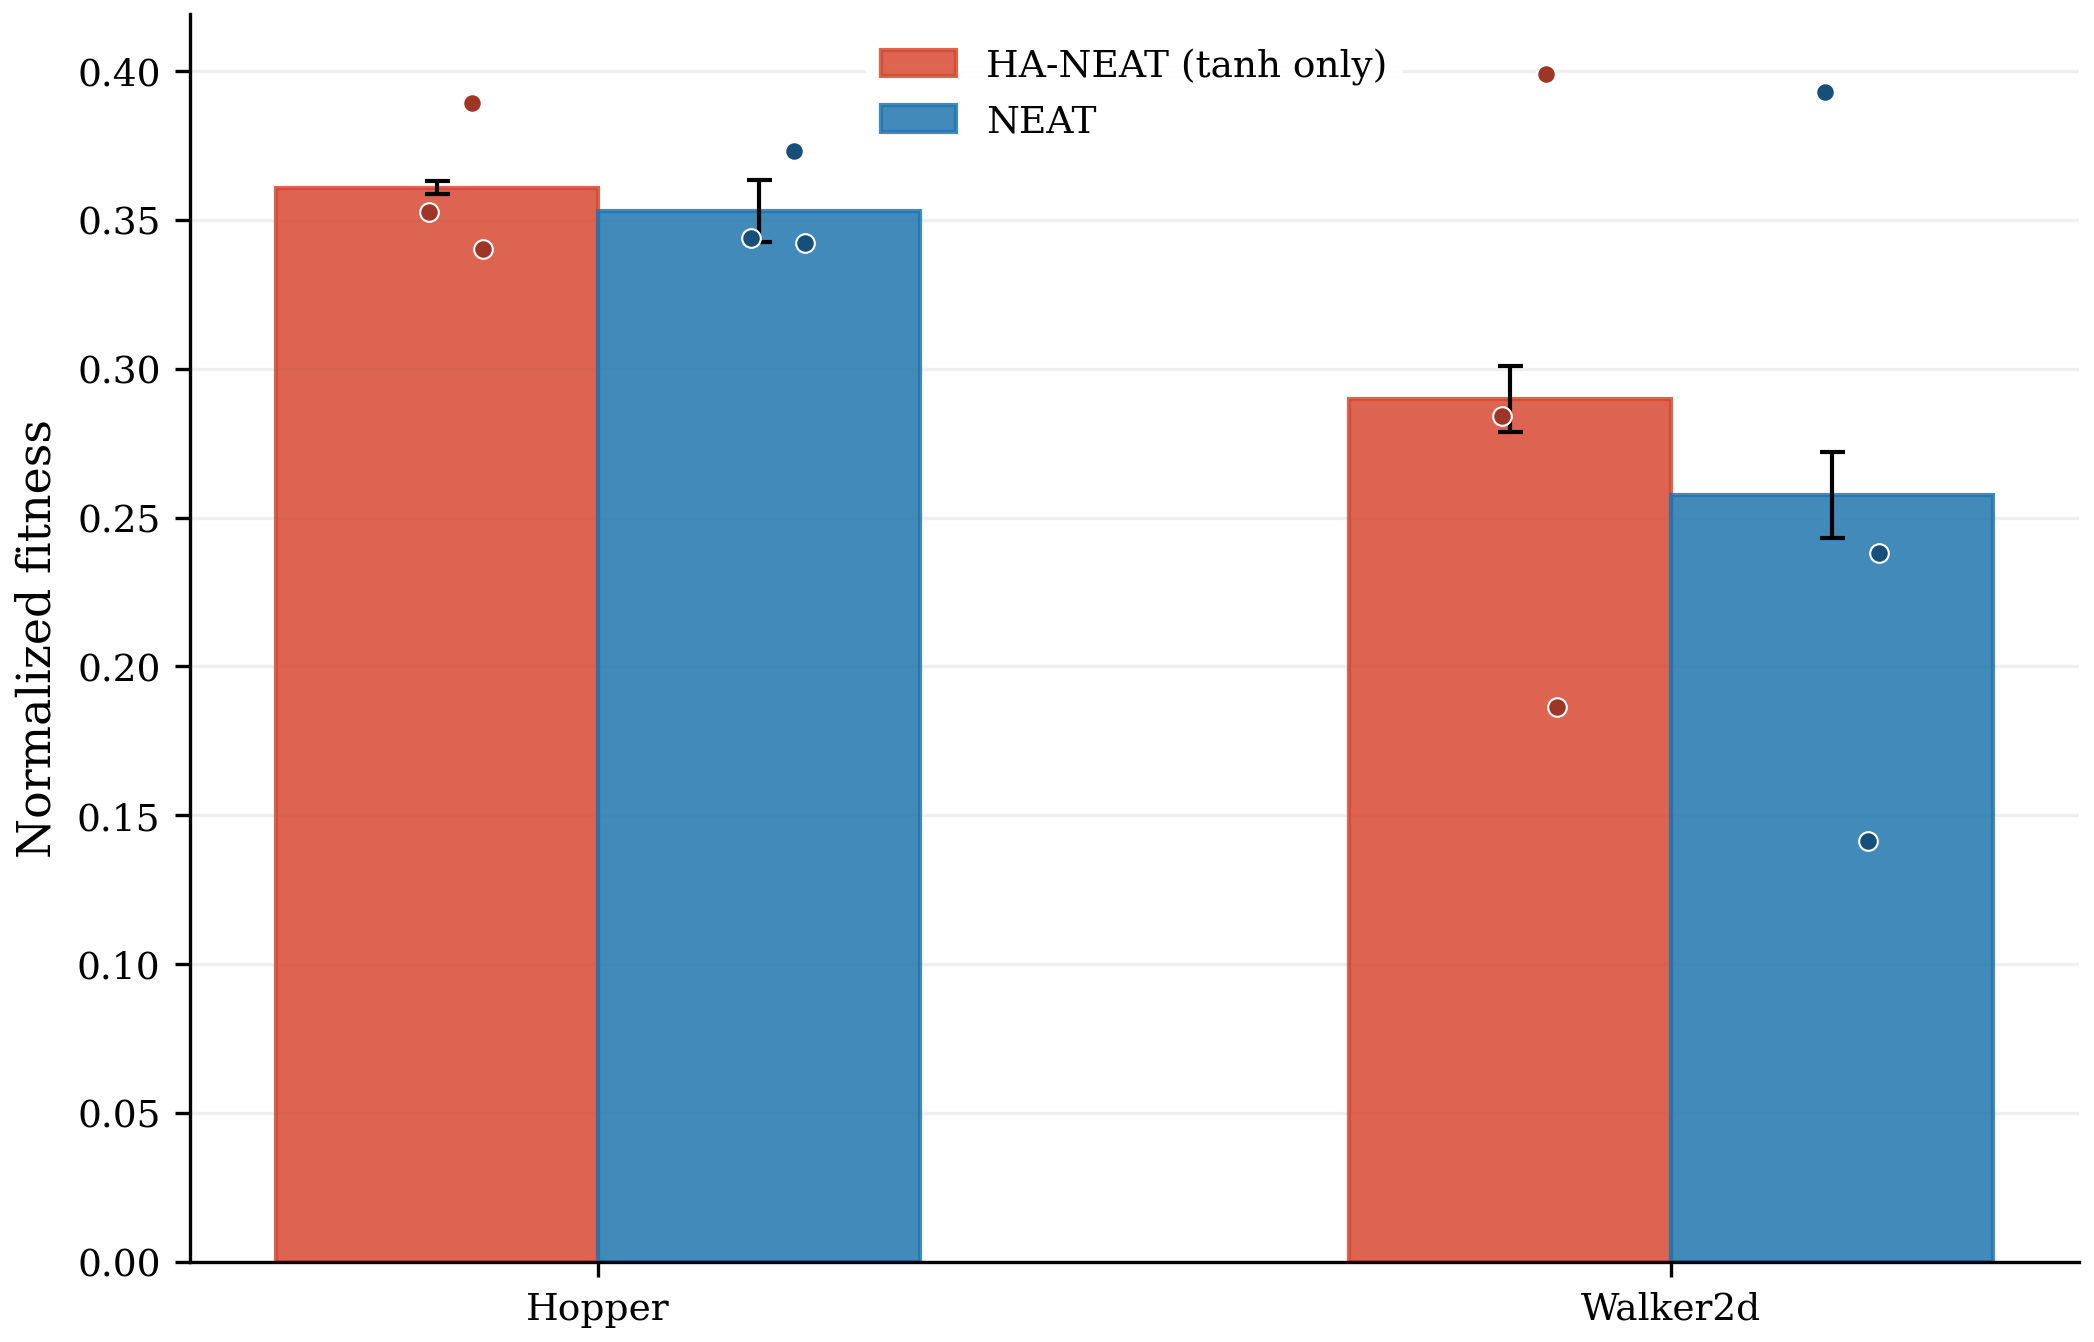
\includegraphics[width=0.75\textwidth]{Figures/multi_task_neat_vs_haneat_ablation_evaluation_normalized.png}
\caption{Mean normalized evaluation fitness over 30 episodes for Hopper and Walker2D in the ablation experiment. Bars show pooled means with SEM error bars, and dots indicate individual seed means.}
\label{fig:ablation-evaluation}
\end{figure}

% On re-evaluation the training-time gap narrows. The ablation actually scores slightly higher than NEAT on both tasks, though the seed-level variance is large, particularly on Walker2D where individual seed means range from 706 to 1966 for NEAT and from 932 to 1996 for the ablation. Table~\ref{tab:ablation-reeval-results} shows that Hopper is nearly id, while Walker2D exhibits substantial spread and no meaningful separation.
In Figure \ref{fig:ablation-evaluation} shows that the performance of both set of networks are nearly identcial, while Walker2D shows some spread.
On re-evaluation the training-time gap narrows.
The HA-NEAT ablation scores slightly higher than NEAT on both individual tasks, and the aggregate normalized minimum tells the same story.
But the seed-level variance is large, particularly on Walker2D where individual seed means range from 706 to 1966 for NEAT and from 932 to 1996 for the ablation.
A difference of 0.046 against a shared standard deviation of 0.101 is not meaningful.


\subsubsection{Statistical comparison}

With only three seeds per method, statistical power is limited.
Table~\ref{tab:ablation-statistics} reports two non-parametric tests on seed-level means, plus effect sizes.

\begin{table}[h]
\centering
\caption{Statistical tests on seed-level means ($n=3$ vs.\ $n=3$).}
\label{tab:ablation-statistics}
\begin{tabular}{lcccc}
\toprule
Task & Permutation test ($p$) & Mann--Whitney U ($p$) & Cohen's $d$ & Interpretation \\
\midrule
Hopper & 0.70 & 1.00 & -0.36 (small) & No significant difference \\
Walker2D & 0.70 & 0.70 & -0.28 (small) & No significant difference \\
\bottomrule
\end{tabular}
\end{table}

Neither task shows a significant difference (permutation $p = 0.70$ for both, Mann--Whitney $p = 0.70$--1.00).
Effect sizes are small: Cohen's $d$ of $-0.36$ on Hopper and $-0.28$ on Walker2D.
One might be tempted to pool all 90 episodes per method and run a $t$-test, which does produce a lower $p$-value on Walker2D (Welch's $t$, $p = 0.08$).
But episodes from the same seed share the same genome, so they are not independent observations.
The proper unit of analysis is the seed-level mean, and at $n = 3$ the tests simply lack power to detect anything short of a very large effect.

Three seeds is a real limitation.
Each ablation run takes [PLACEHOLDER: wall-clock time] on a single GPU, and scaling to 20--30 seeds was not feasible within our compute budget.
Rather than relying on $p$-values that were never going to be informative at this sample size, we draw on three pieces of evidence together.
The training curves show overlapping trajectories across 500 generations, not just similar endpoints.
The re-evaluation effect sizes are small.
And the direction of the non-significant difference actually favors the ablation slightly over NEAT, the opposite of what we would expect if HA-NEAT's machinery provided any advantage on its own.

Taken together, OriginConn and marker reassignment without activation diversity do not improve performance.
The ablation slightly underperforms NEAT during training and performs comparably on re-evaluation.
At this small sample size ($n=3$) this pointed toward activation diversity rather than the surrounding infrastructure; the larger pop200 study (Section~\ref{sec:pop200}, $n=30$ per condition) revises that reading, finding no fitness difference between the three conditions yet attributing a structural fingerprint to the HA-NEAT machinery itself, as the pop200 subsections that follow develop. [PLACEHOLDER: include full HA-NEAT bar from final experiment data for direct three-way comparison.
Note the population size mismatch (ablation: pop 1024, main experiment: pop 4096) when interpreting magnitudes.]

\subsection{Multi-task performance comparison}

We compared the best-found normalized-minimum fitness per run across both methods and several configurations.
Table~\ref{tab:aggregate-fitness-versions} collects results across experiment versions.

\begin{table}[h]
\centering
\caption{Aggregate normalized-minimum fitness per method across experiment versions.}
\label{tab:aggregate-fitness-versions}
\resizebox{\textwidth}{!}{%
\begin{tabular}{lllllll}
\toprule
Experiment & Method & Pop & Gens & Seeds & Scores (per seed) & Mean \\
\midrule
v3 & NEAT & 2048 & 500 & 42, 123 & 0.358, 0.341 & 0.349 \\
v3 & HA-NEAT & 2048 & 500 & 42, 123 & 0.342, 0.484 & 0.413 \\
v4 & NEAT & 4096 & 1000 & 42 & 0.399 & 0.399 \\
v4 & HA-NEAT & 4096 & 1000 & 42, 123 & 0.473, 0.457 & 0.465 \\
final & NEAT & 4096 & 2000 & 42, 123, 75, 7, 21 & [PLACEHOLDER] & [PLACEHOLDER] \\
final & HA-NEAT & 4096 & 2000 & 42, 123, 75, 7, 21 & [PLACEHOLDER] & [PLACEHOLDER] \\
\bottomrule
\end{tabular}%
}
\end{table}



In the preliminary v3 runs, HA-NEAT averaged 0.413 across two seeds, compared to 0.349 for NEAT, a gap of 0.064 normalized units.
Most of that gap came from one strong HA-NEAT run (seed 123: 0.484).
In the v4 configuration (pop=4096, 1000 generations), the single completed NEAT run reached 0.399, while the two HA-NEAT runs averaged 0.465.
The final experiment, with 5 seeds per method, will show whether this advantage holds with a larger sample. [PLACEHOLDER: final experiment mean +/- std for NEAT and HA-NEAT.
Update this paragraph once complete.] Across both experiment versions, HA-NEAT tended toward higher aggregate fitness, though with high cross-seed variance in both methods.
The aggregate number alone does not tell us whether both tasks improved or whether one task carried the other.

\subsection{The pop200 study}
\label{sec:pop200}
The experiments in Sections~\ref{sec:pop200} onward use a fixed, larger-sample design: population 200, 750 generations, and 30 independent random seeds per condition.
Three conditions were compared: standard NEAT (tanh only), HA-NEAT (activation set tanh, sigmoid, relu, sin, identity), and an ablation that runs HA-NEAT's full machinery restricted to tanh.
All runs share the multi-task Hopper$+$Walker2D problem and the normalized-minimum objective $\mathrm{fit} = \min(r_{\text{hopper}}/3000,\, r_{\text{walker2d}}/5000)$.

Across the three conditions, the best-found normalized-minimum fitness showed no significant difference (Kruskal--Wallis $H = 1.48$, $p = 0.476$).
We ran the analyses that follow \emph{after} this null result.
They ask a second question: whether conditions that reach equal fitness do so with equivalent internal structure and task balance.
These are exploratory, post-hoc analyses, and we frame them as such throughout.
\label{res:pop200-fitness}

\subsection{Genome complexity and generational dynamics}
\label{sec:pop200-complexity}

Because the three conditions reached statistically indistinguishable fitness (Section~\ref{res:pop200-fitness}), we examined whether they arrived there with equivalent genome structure.
This tests one reading of the null: that activation diversity substitutes for topological complexity.
For each of the 90 champion genomes (30 per condition) we counted hidden nodes and active connections from the raw genome arrays.
The 17 input and 6 output nodes are fixed by the task and excluded from the hidden-node count.

The number of hidden nodes in the final champions differed across conditions (Figure~\ref{fig:pop200-hidden}).
NEAT champions carried a median of 2.0 hidden nodes (IQR $[1.0, 3.0]$), HA-NEAT 1.0 ($[0.0, 2.0]$), and the ablation 0.0 ($[0.0, 2.0]$); a Kruskal--Wallis test rejected equality of the three distributions ($H = 7.45$, $p = 0.024$, $\varepsilon^2 = 0.063$).
Holm-corrected pairwise Mann--Whitney tests localized the effect to a single contrast: NEAT versus the ablation ($p = 0.030$, Cliff's $\delta = 0.38$, medium), while NEAT versus HA-NEAT ($p = 0.10$) and HA-NEAT versus the ablation ($p = 0.52$) were not significant.
Connection counts did not differ across conditions (medians 48.5 / 51.5 / 47.0; $H = 2.82$, $p = 0.244$; Figure~\ref{fig:pop200-conns}).

The per-generation trajectories from the training logs locate when this gap opens (Figure~\ref{fig:pop200-complexity-gens}).
Best-genome node counts overlapped across all three conditions until roughly generation 300, after which NEAT rose above both HA-NEAT variants, reaching a final-window mean of 26.6 total nodes (including the 23 fixed input/output nodes) against 24.7 (HA-NEAT) and 24.0 (ablation).
Connection counts pruned in lockstep across all three conditions, falling from roughly 100 to 40--44 by the final window.
Species counts saturated near the same ceiling in every condition (final-window means 9.97 / 9.97 / 9.97; Kruskal--Wallis $H = 0.11$, $p = 0.945$; Figure~\ref{fig:pop200-species}), consistent with the configured target of $\approx 10$ species.
The conditions therefore converged to equal fitness while ending at different topologies: the ablation and HA-NEAT settled on more compact networks than NEAT.

\begin{figure}[h]
\centering
\begin{minipage}[t]{0.49\textwidth}
\centering
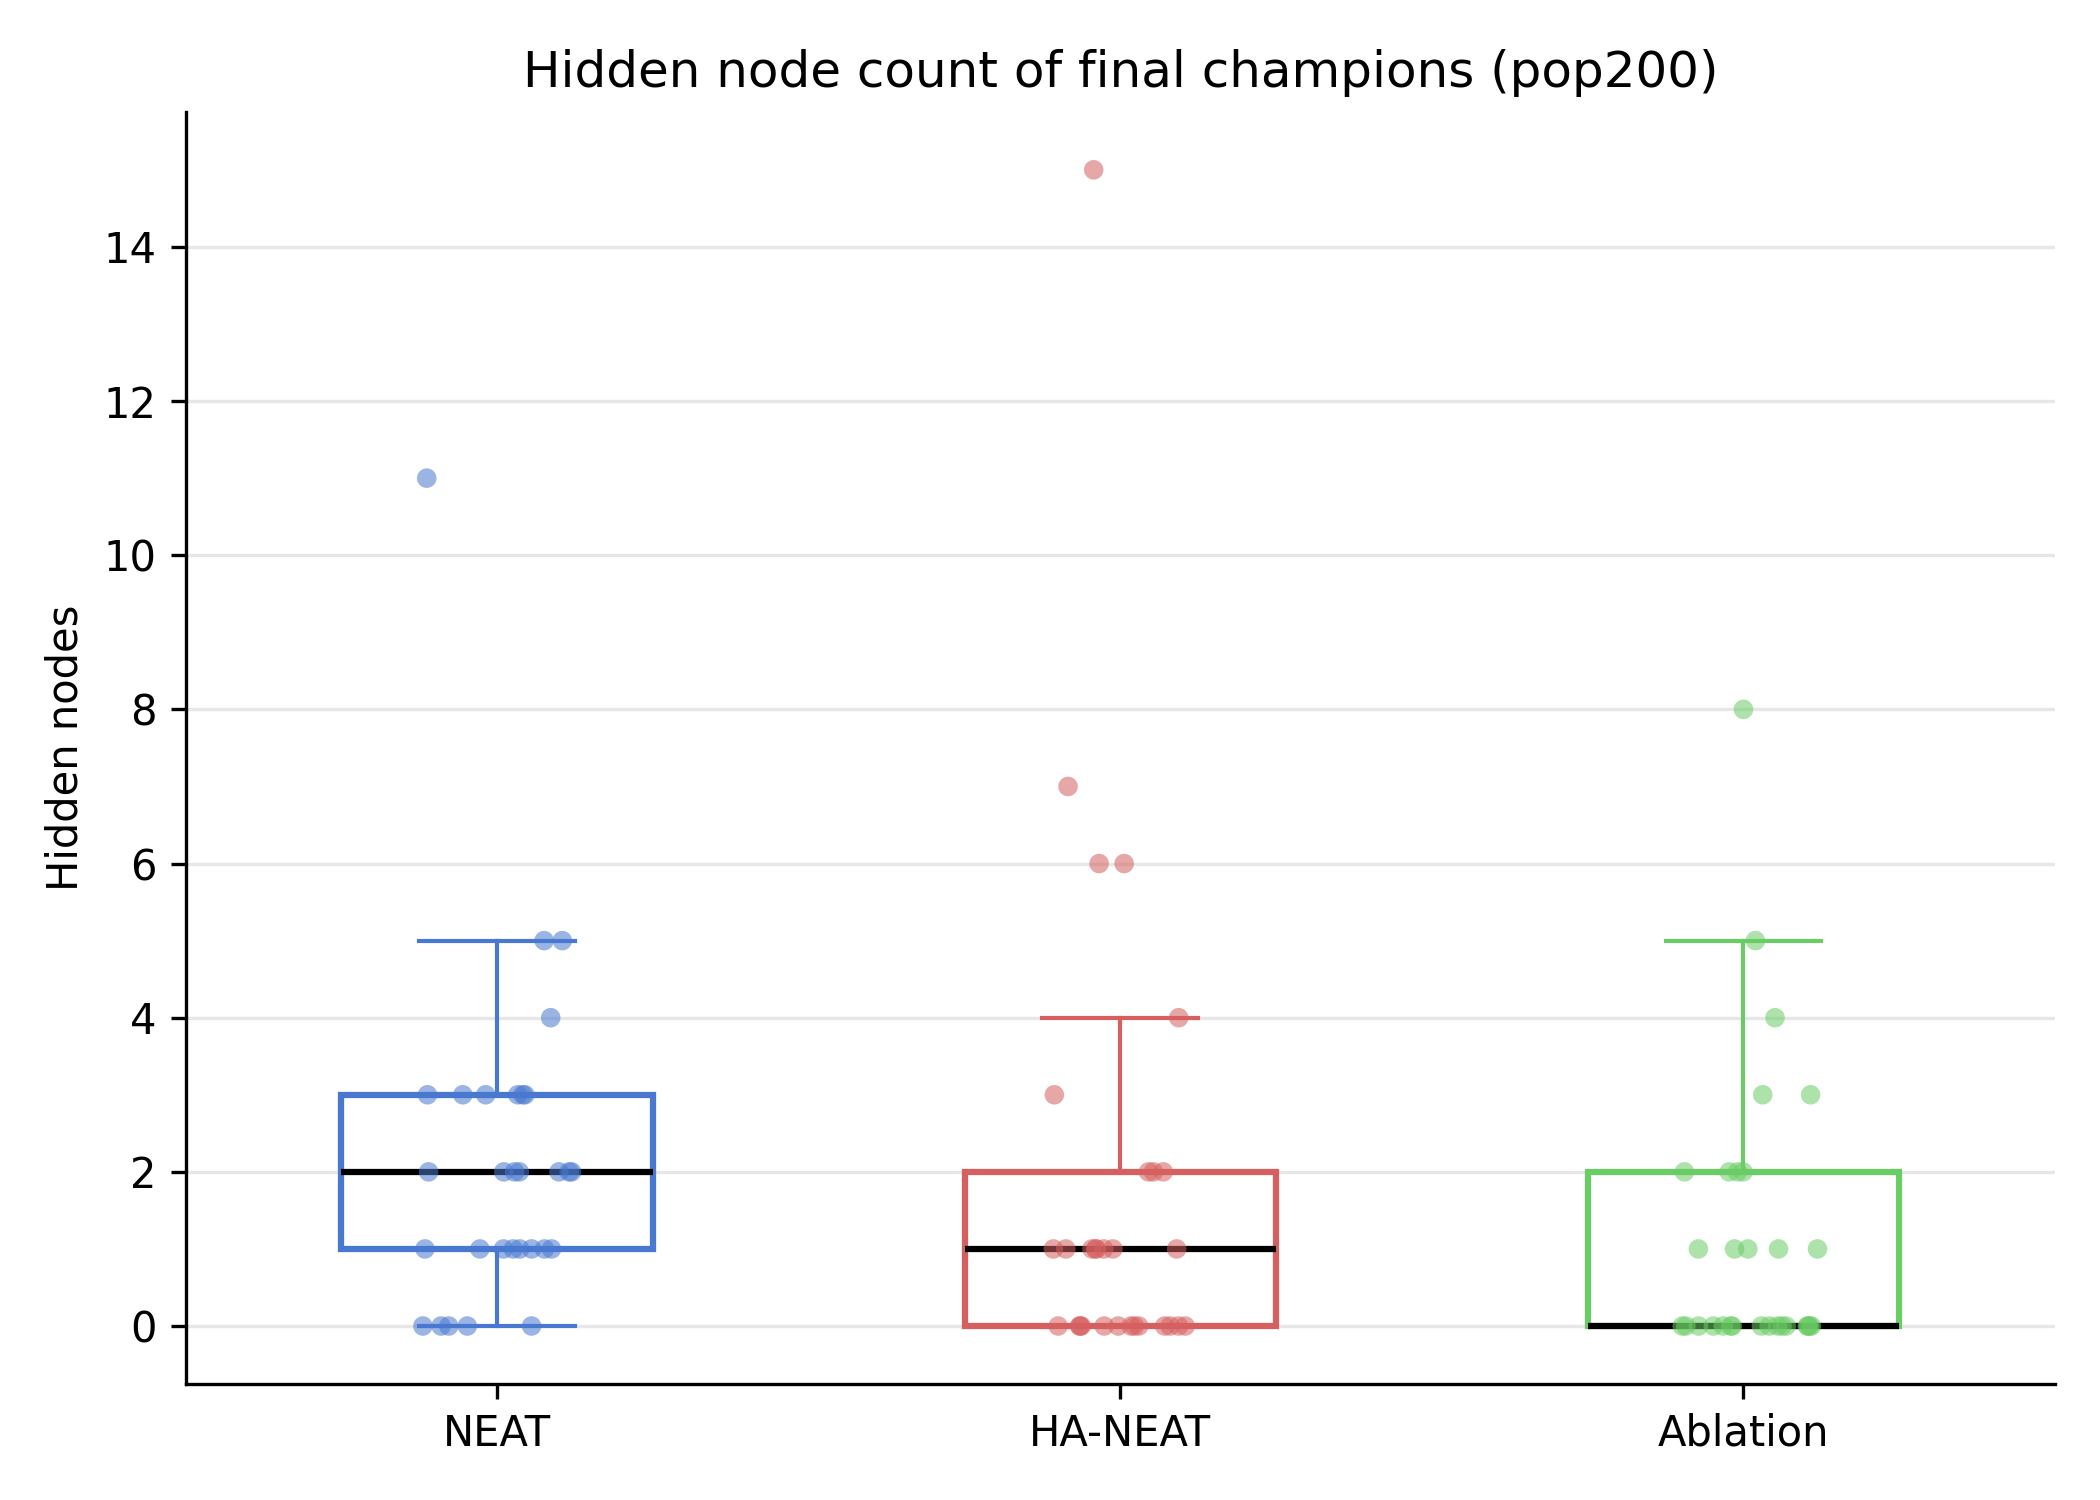
\includegraphics[width=\textwidth]{Figures/complexity_hidden_nodes.png}
\textit{(a) Hidden nodes per champion.}
\label{fig:pop200-hidden}
\end{minipage}\hfill
\begin{minipage}[t]{0.49\textwidth}
\centering
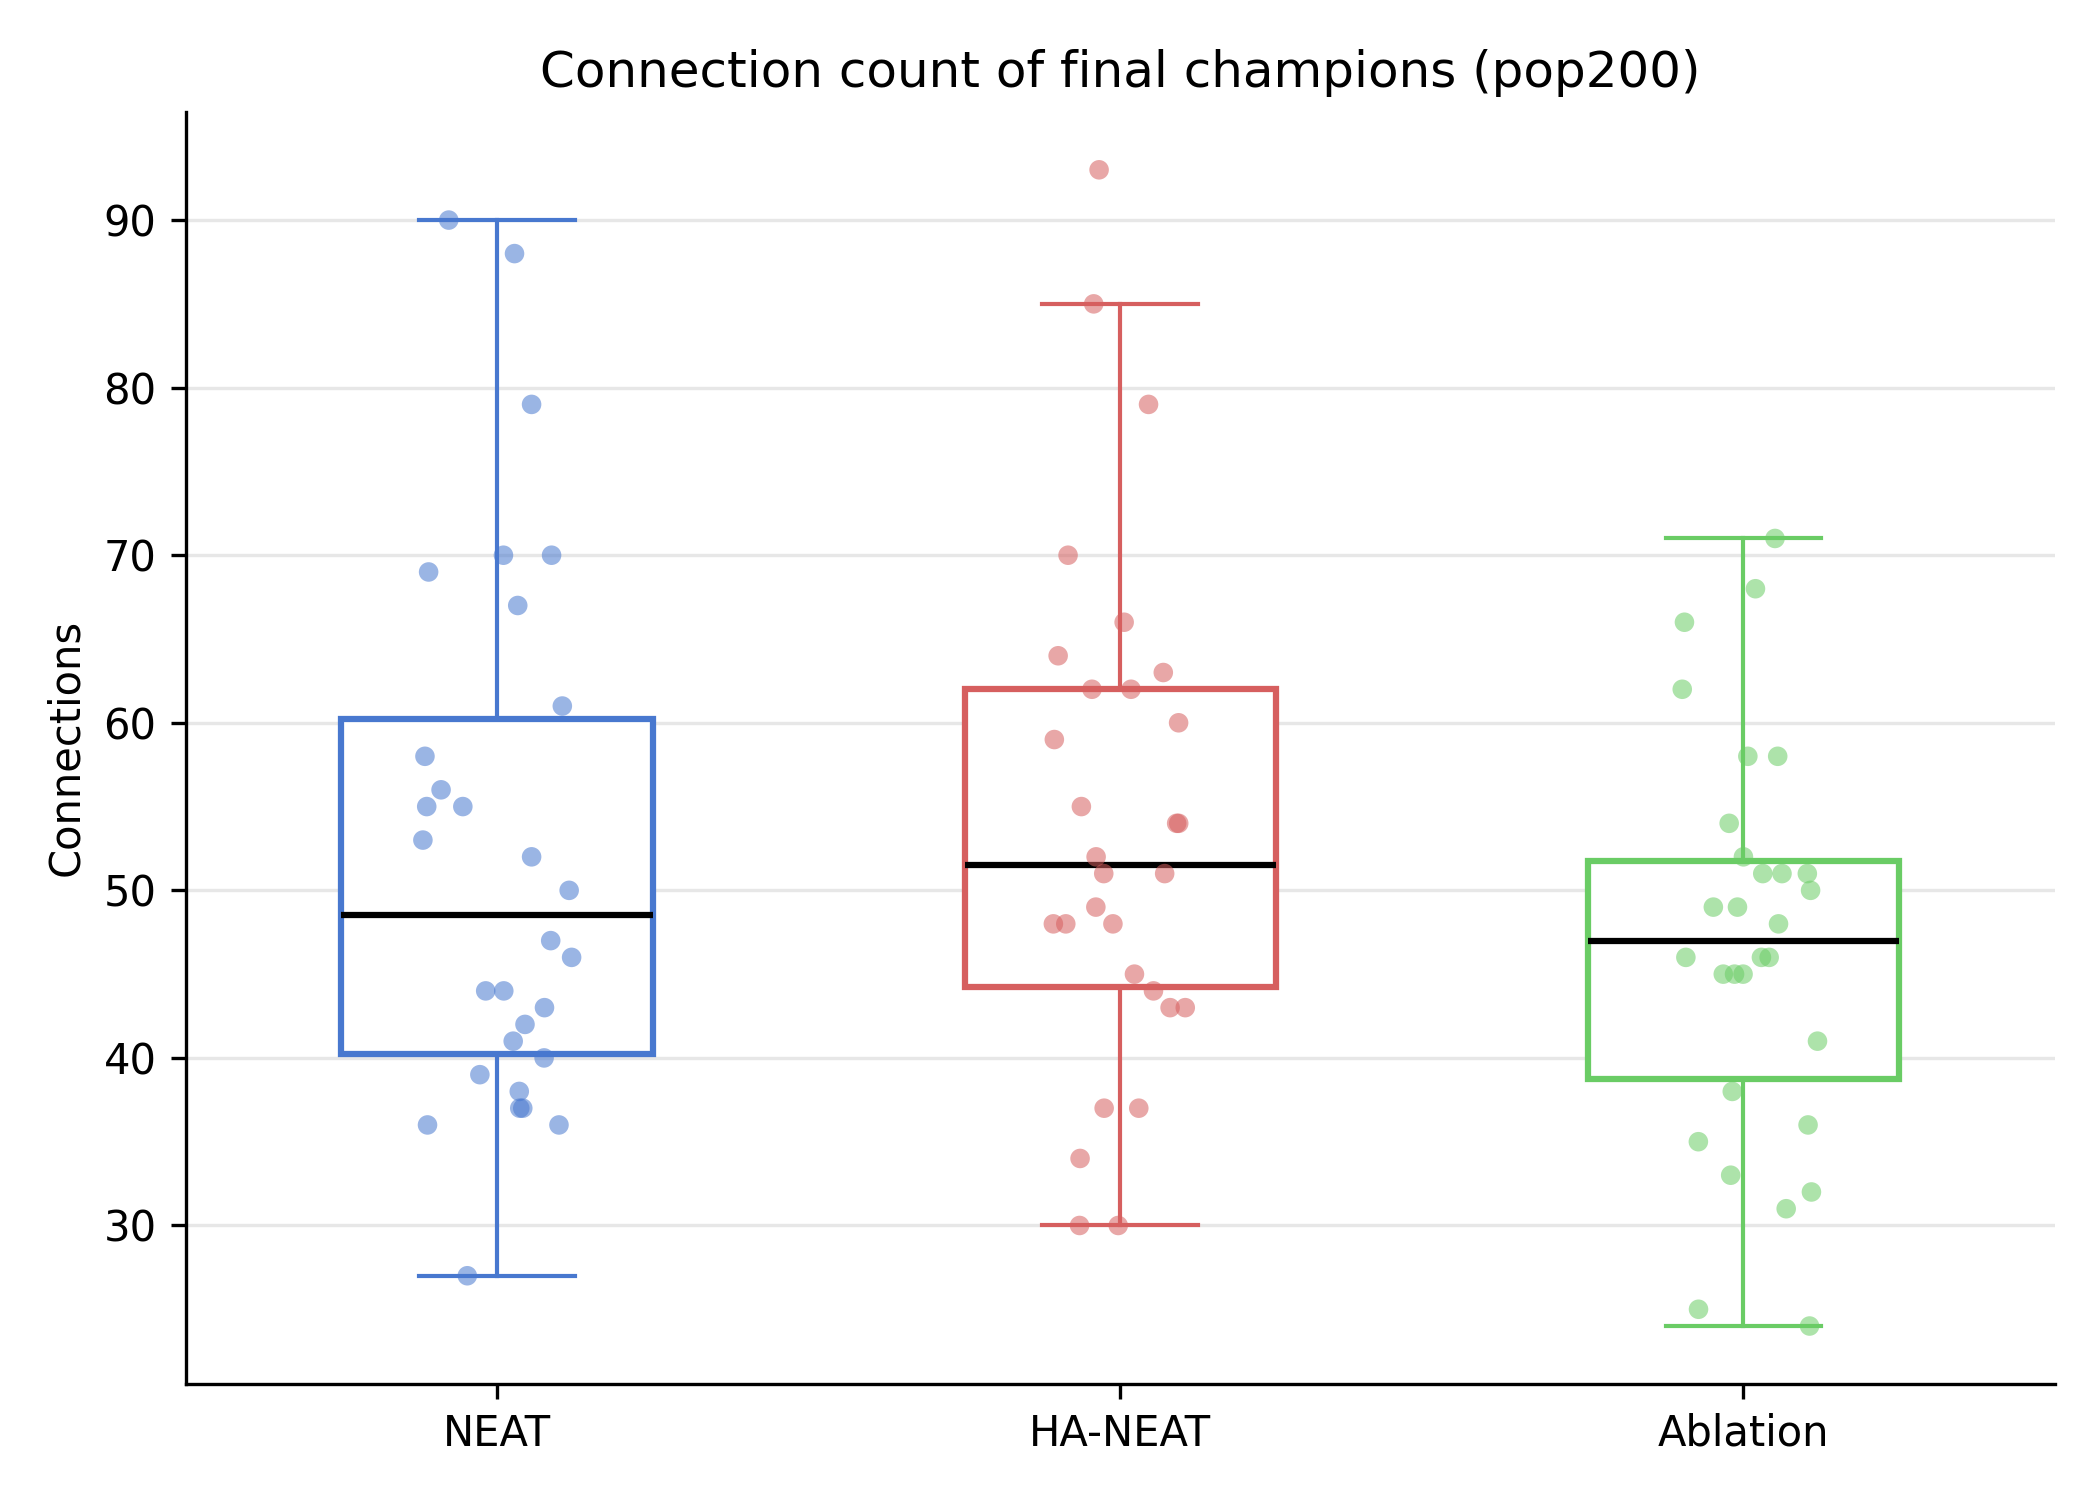
\includegraphics[width=\textwidth]{Figures/complexity_connections.png}
\textit{(b) Active connections per champion.}
\label{fig:pop200-conns}
\end{minipage}
\caption{Final-champion complexity in the pop200 study ($n=30$ per condition). (a) Hidden-node
distributions differ across conditions (Kruskal--Wallis $p = 0.024$), driven by the NEAT vs.\
ablation contrast; (b) connection counts do not ($p = 0.244$).}
\end{figure}

\begin{figure}[h]
\centering
\begin{minipage}[t]{0.49\textwidth}
\centering
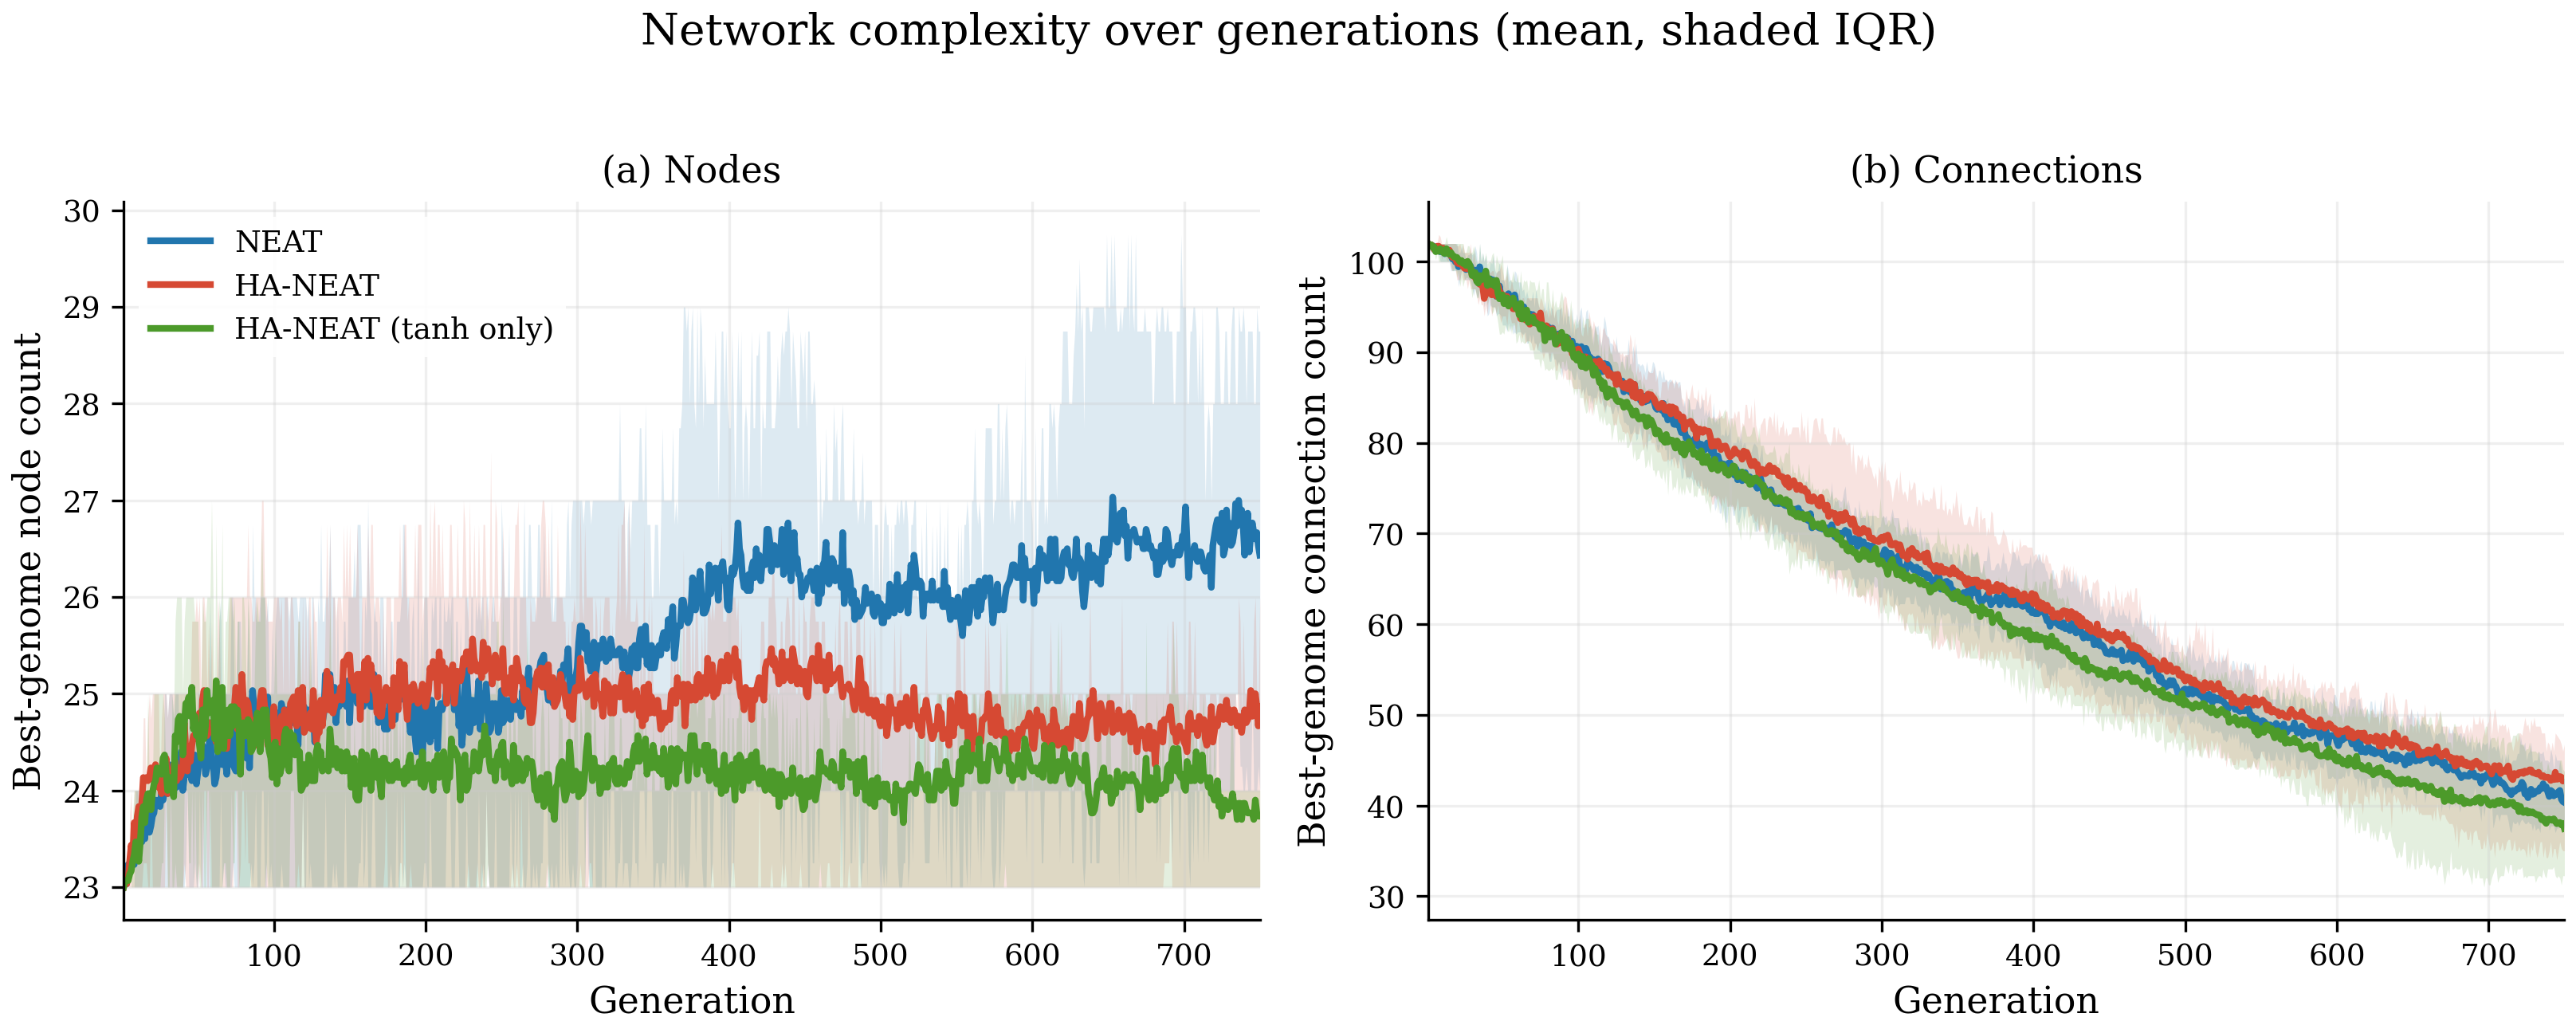
\includegraphics[width=\textwidth]{Figures/complexity_over_generations.png}
\textit{(a) Best-genome node and connection counts over generations.}
\label{fig:pop200-complexity-gens}
\end{minipage}\hfill
\begin{minipage}[t]{0.49\textwidth}
\centering
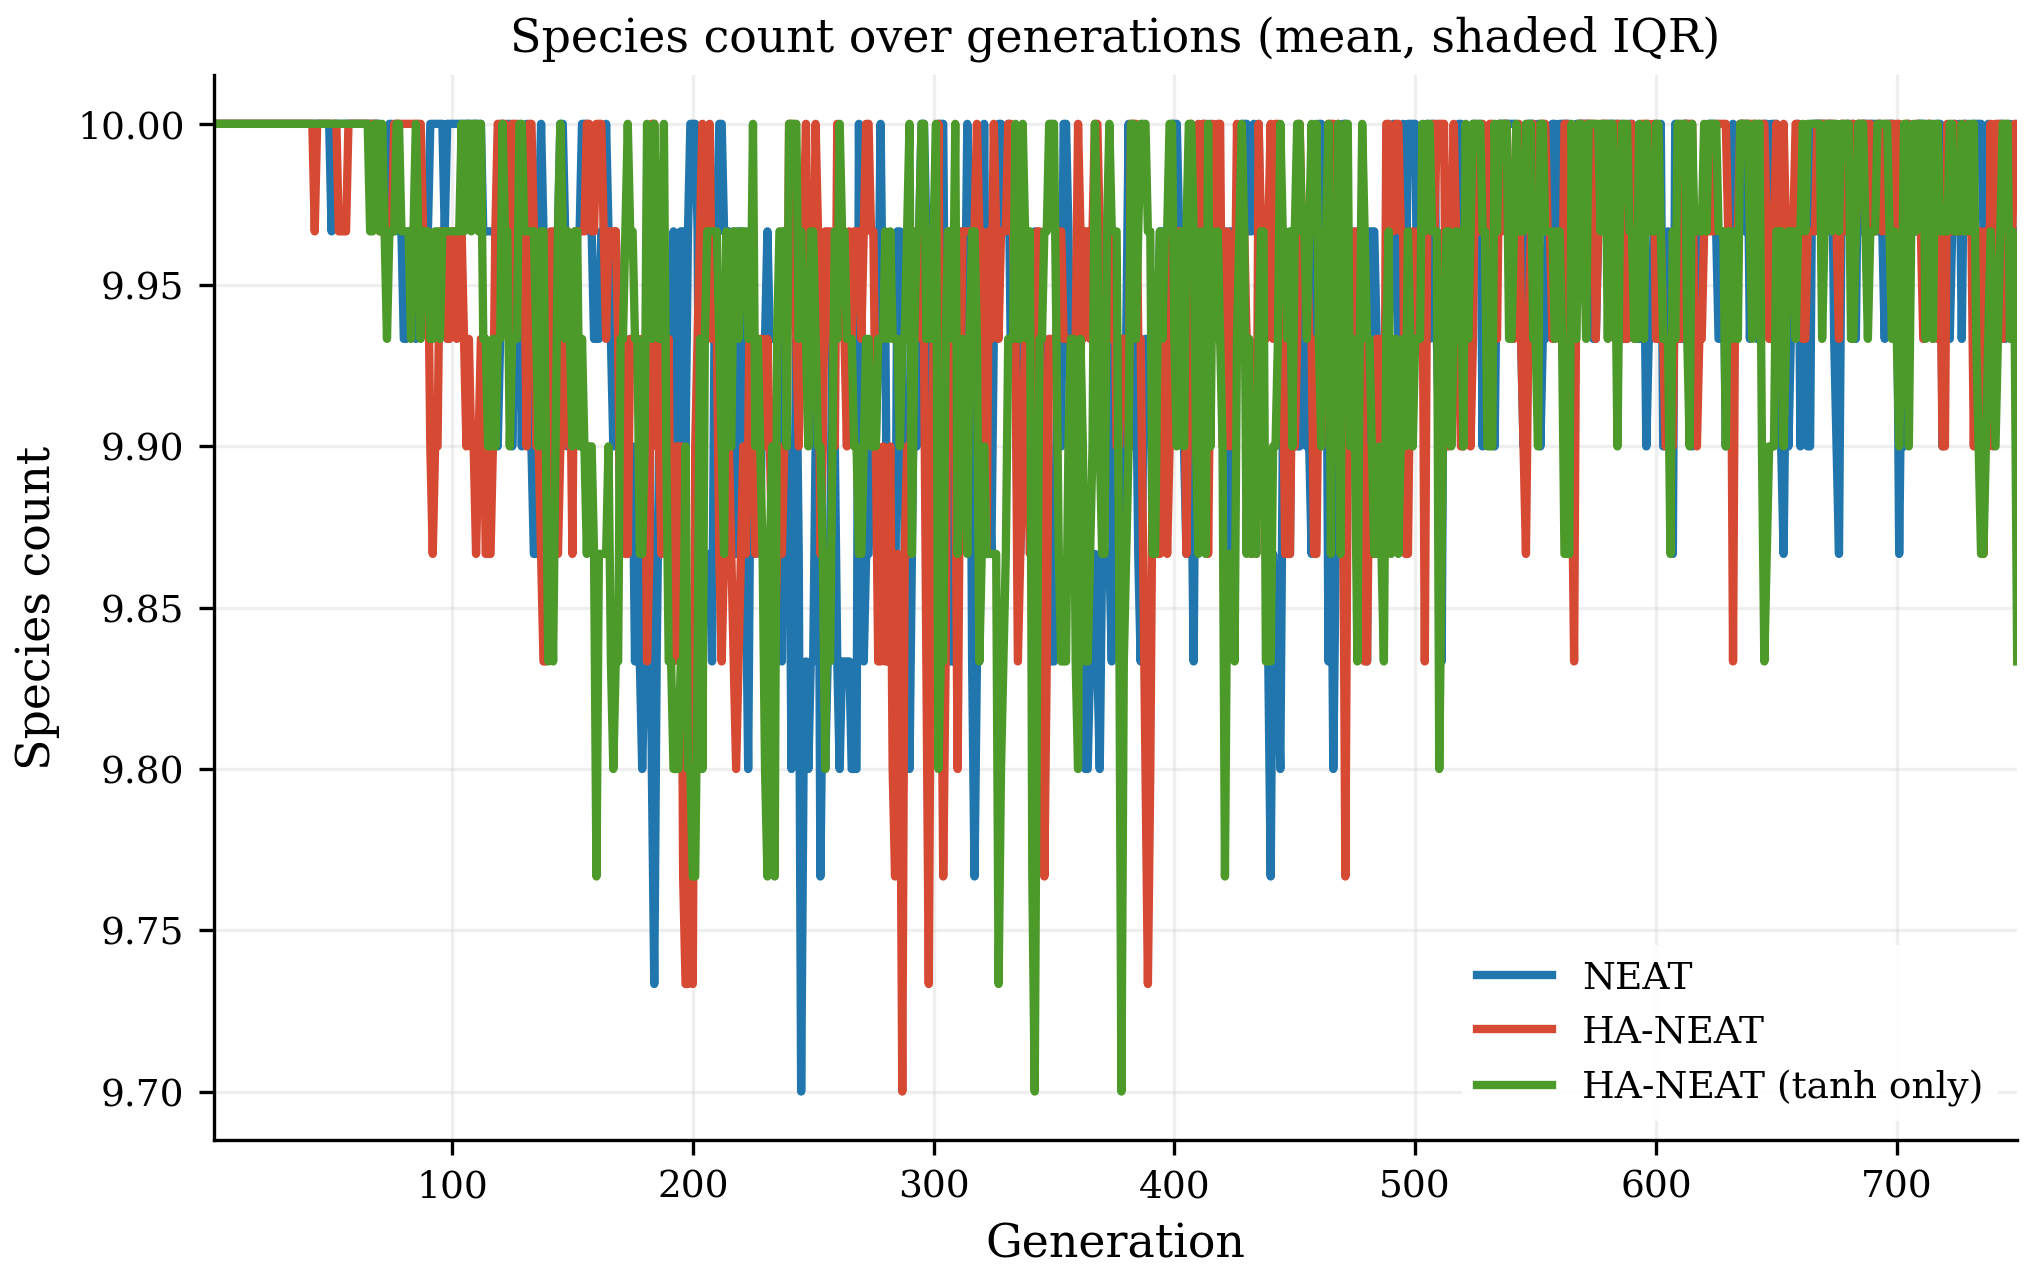
\includegraphics[width=\textwidth]{Figures/species_over_generations.png}
\textit{(b) Species count over generations.}
\label{fig:pop200-species}
\end{minipage}
\caption{Generational dynamics in the pop200 study. Lines are across-seed means; bands are the
inter-quartile range. (a) Node counts diverge only after $\approx$ generation 300 and connection
counts prune in lockstep; (b) species counts saturate near the configured ceiling in all
conditions.}
\FloatBarrier
\end{figure}

\subsection{Per-task trade-off and multi-task pressure}
\label{sec:pop200-tradeoff}

The aggregate fitness leaves open whether both tasks improved together or one task set the score throughout; to resolve this we plotted each champion's normalized Hopper score against its normalized Walker2D score and compared the per-task balance across conditions.
Per-task scores are the normalized 20-episode returns from re-evaluation; $\min$ of the two is the training objective.

Champions in all three conditions clustered in a narrow vertical band at normalized Hopper $\approx 0.33$--$0.35$, while Walker2D spread across a wider range and set the minimum for the large majority of genomes (Figure~\ref{fig:pop200-tradeoff}).
Walker2D was the binding task for 97\% of NEAT champions, 83\% of HA-NEAT, and 90\% of the ablation.
The per-genome imbalance $|r_{\text{hopper}} - r_{\text{walker2d}}|$ did not differ across conditions (medians 0.159 / 0.117 / 0.142; Kruskal--Wallis $H = 3.39$, $p = 0.184$).
The Hopper band sits at $0.34 \times 3000 \approx 1000$ raw reward, which for this environment corresponds to roughly 1000 timesteps of the per-step healthy/alive bonus \cite{freeman_brax_2021}.
Across every condition, then, champions solved the multi-task problem with the same lopsided profile: a saturated Hopper score and a Walker2D score that carried the aggregate.

\begin{figure}[h]
\centering
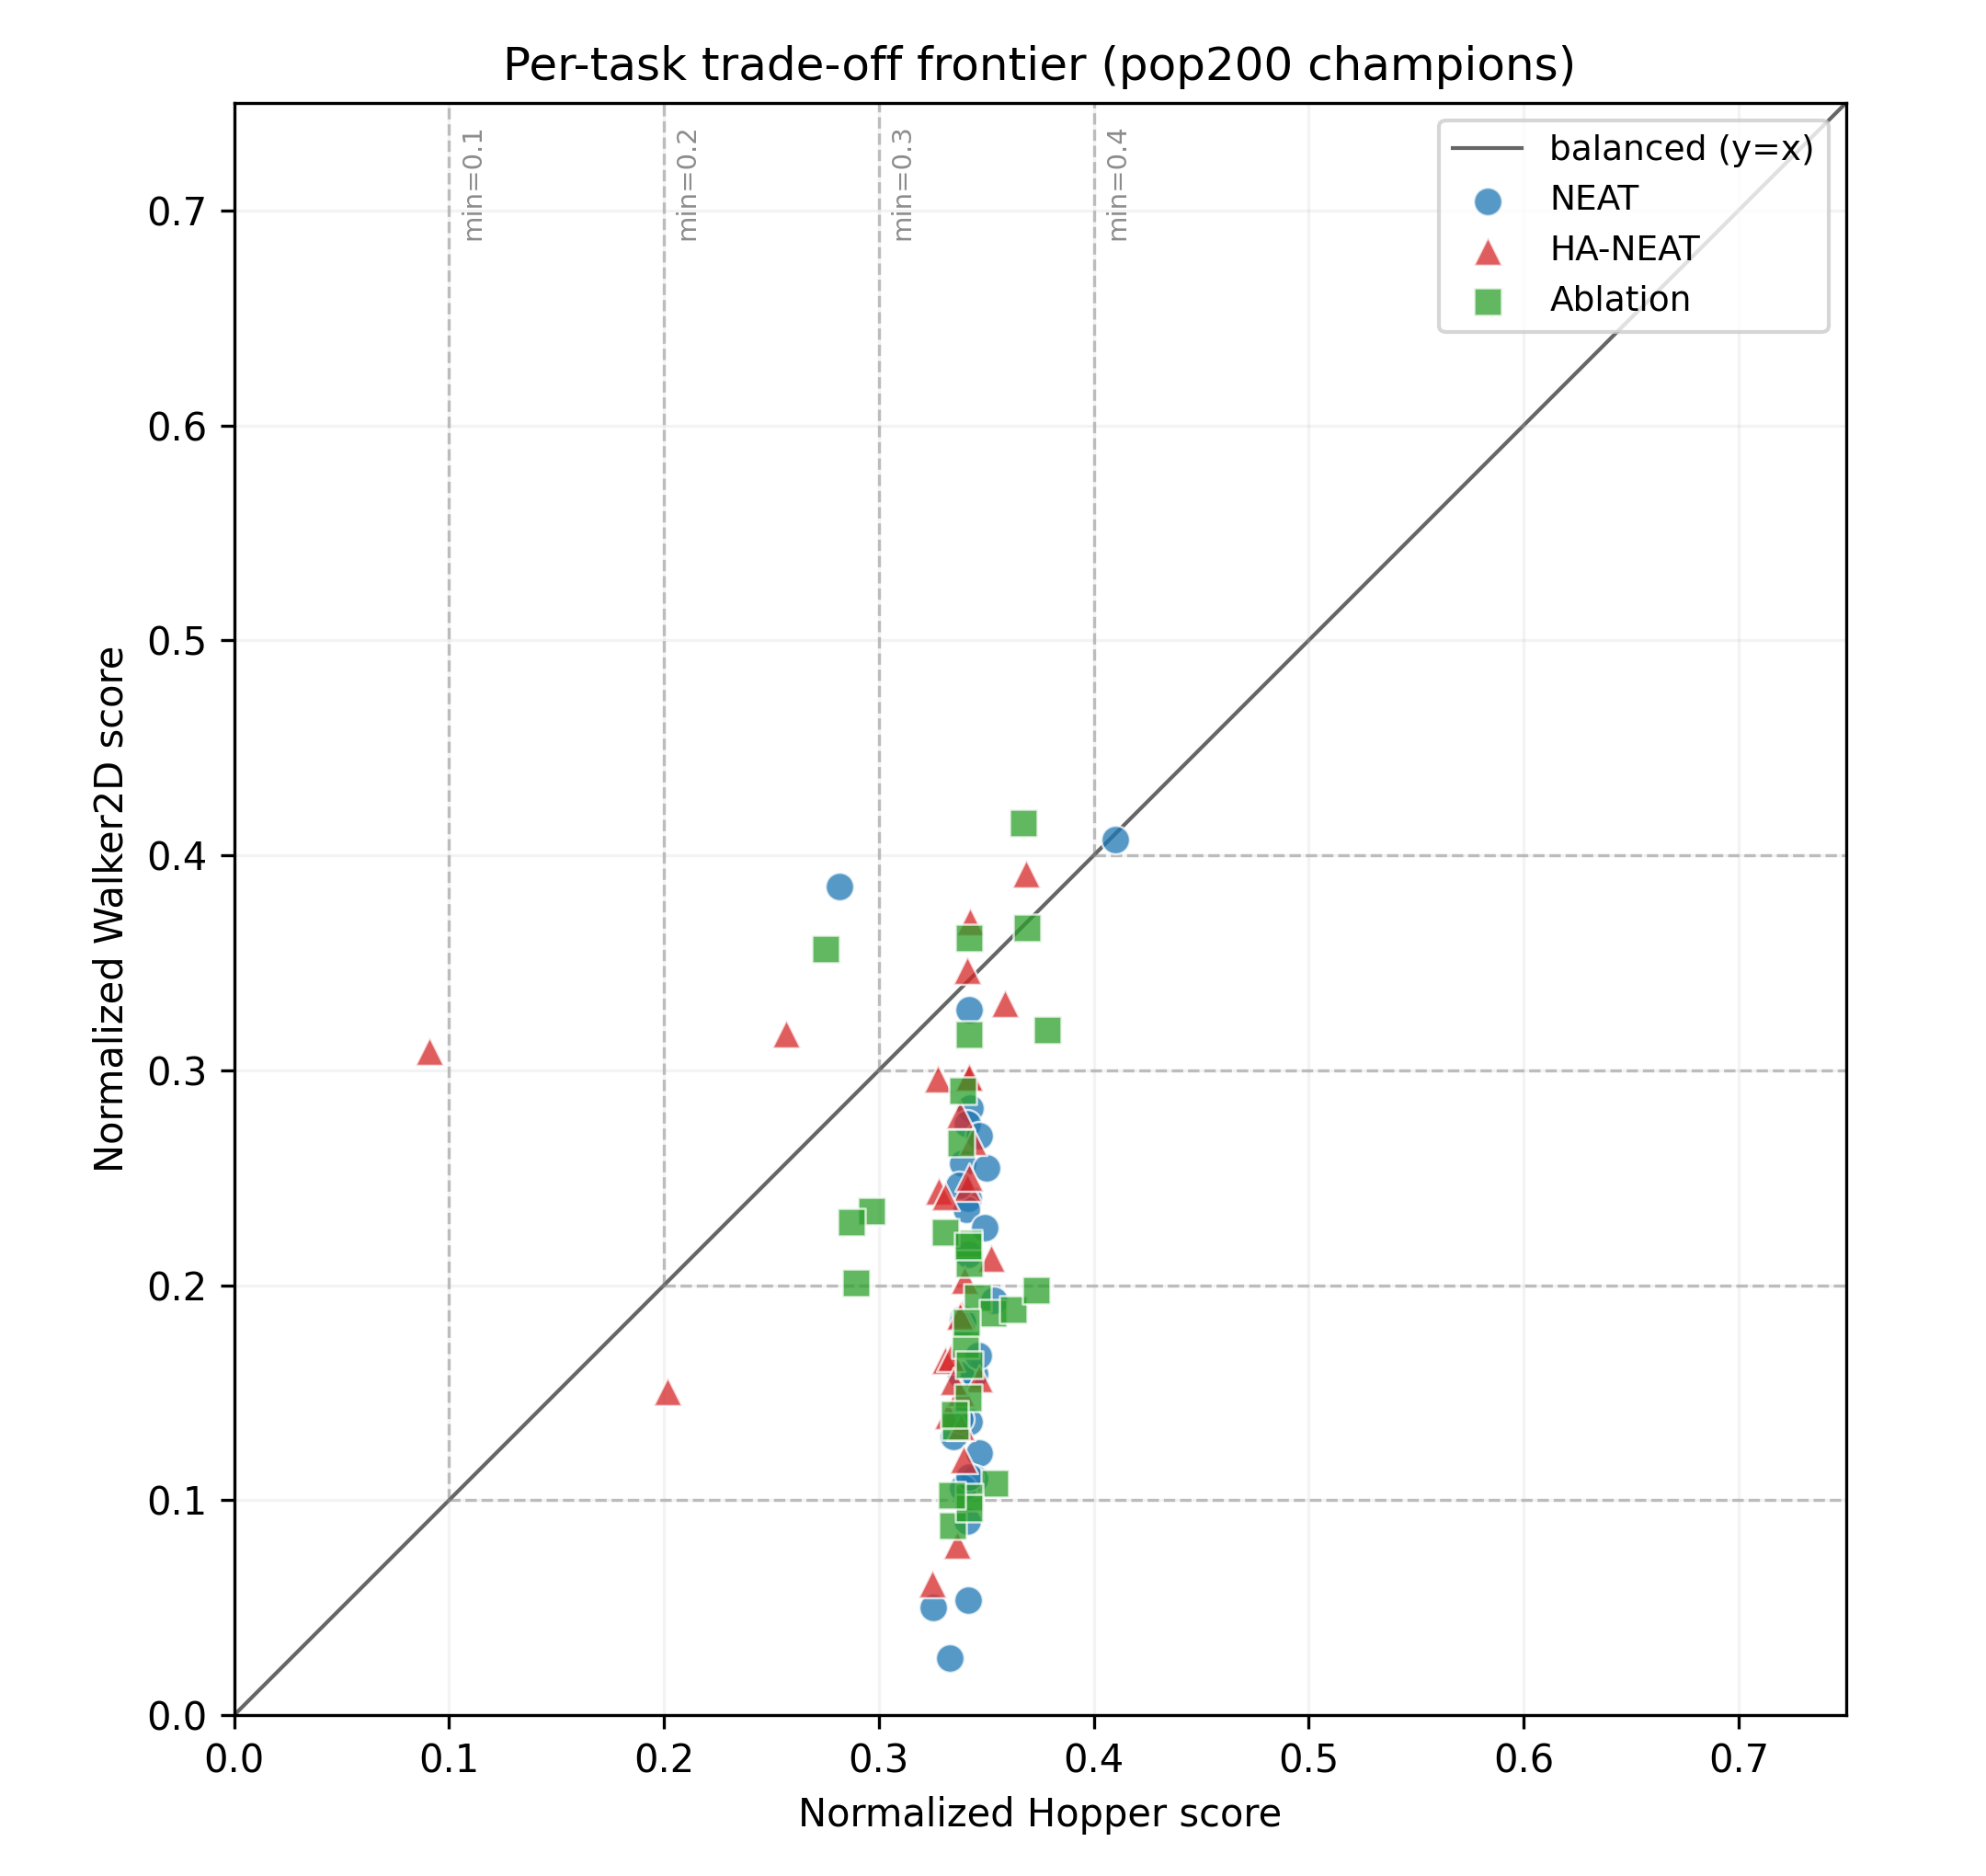
\includegraphics[width=0.75\textwidth]{Figures/tradeoff_frontier.png}
\caption{Per-task trade-off frontier in the pop200 study ($n=30$ per condition). Each point is a
champion's normalized Hopper score (x) against its normalized Walker2D score (y). Champions cluster
in a vertical band at Hopper $\approx 0.33$--$0.35$ in all conditions; Walker2D is the binding task
for 83--97\% of champions. Per-genome imbalance does not differ across conditions
(Kruskal--Wallis $p = 0.184$).}
\label{fig:pop200-tradeoff}
\FloatBarrier
\end{figure}

\subsection{Activation-function usage within HA-NEAT}
\label{sec:pop200-activation}

If activation diversity is the ingredient that HA-NEAT contributes, its champions should both use the non-tanh activations and be rewarded for doing so; we examined the activation composition of HA-NEAT's hidden nodes and its relationship to fitness.
Of the 30 HA-NEAT champions, 17 evolved at least one hidden node; the remaining 13 had none, leaving 55 hidden nodes across the informative seeds.

The evolved activations were diverse and rarely defaulted to tanh (Figure~\ref{fig:pop200-activation-dist}).
Among the 55 hidden nodes, relu accounted for 27\%, sigmoid 24\%, identity 22\%, sin 16\%, and tanh 11\%.
Neither summary of diversity predicted fitness across the 17 informative champions (Figure~\ref{fig:pop200-activation-fit}): activation entropy showed no monotonic relationship with fitness (Spearman $\rho = -0.05$, $p = 0.84$), nor did the fraction of non-tanh hidden nodes ($\rho = 0.27$, $p = 0.30$).
With only 17 informative genomes these correlation tests are underpowered.
We therefore read the flat correlations as an absence of evidence, not as evidence that diversity is irrelevant.

\begin{figure}[h]
\centering
\begin{minipage}[t]{0.49\textwidth}
\centering
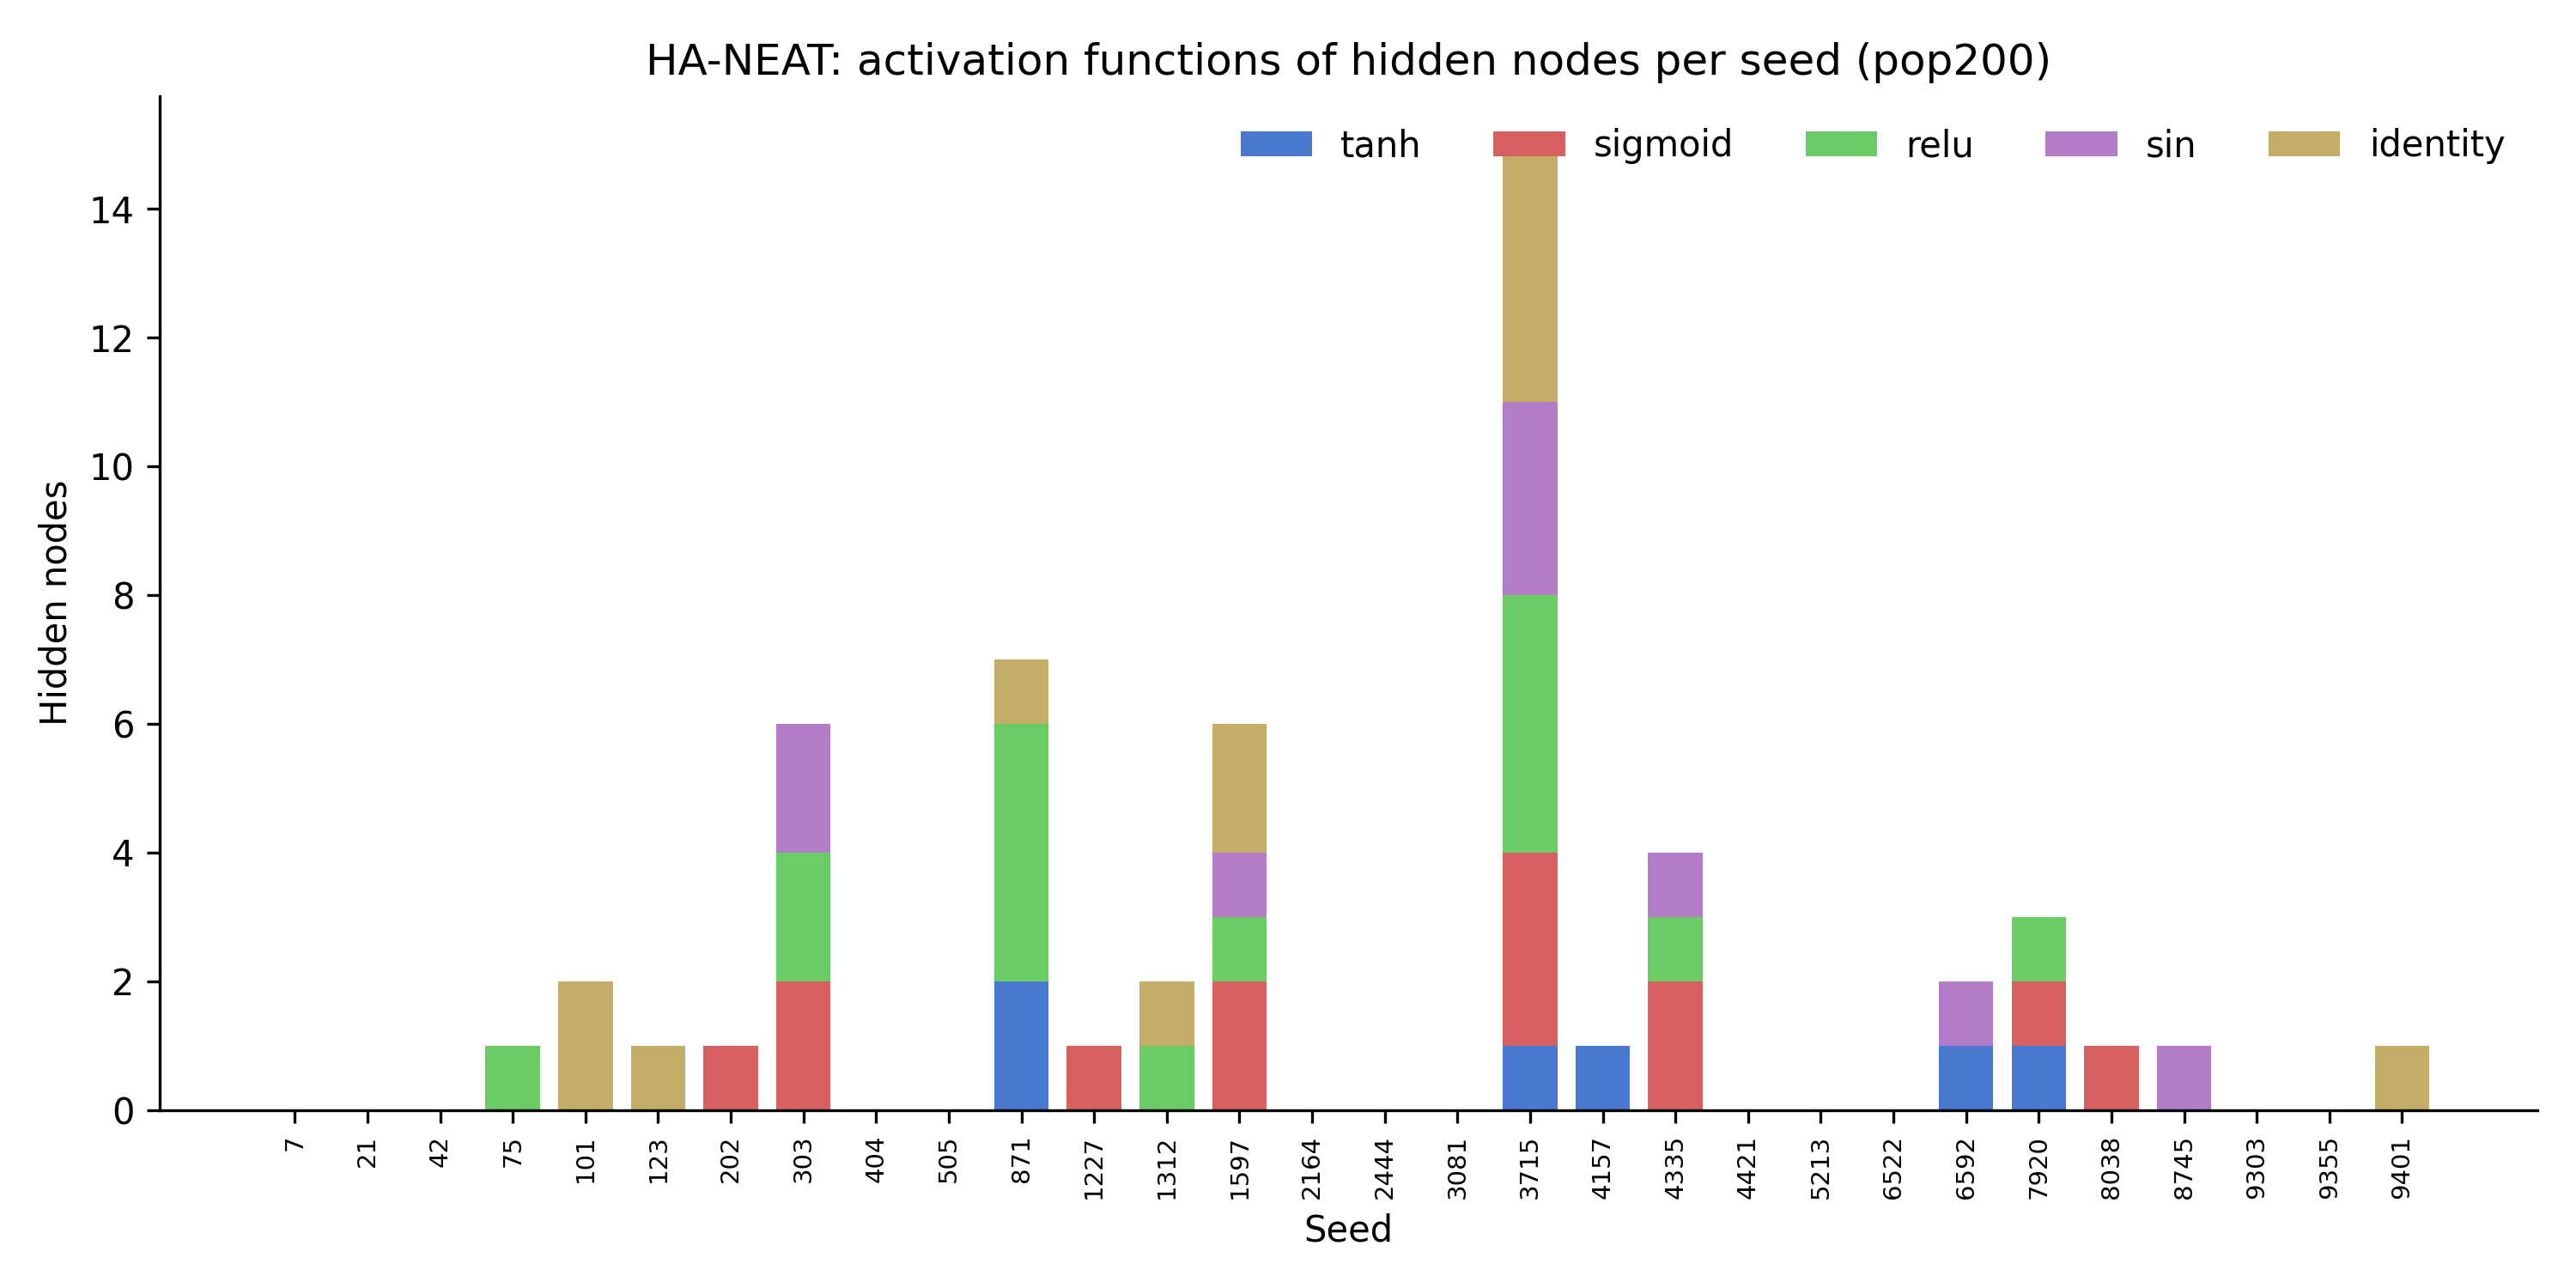
\includegraphics[width=\textwidth]{Figures/haneat_activation_distribution.png}
\textit{(a) Activation composition of the 55 HA-NEAT hidden nodes.}
\label{fig:pop200-activation-dist}
\end{minipage}\hfill
\begin{minipage}[t]{0.49\textwidth}
\centering
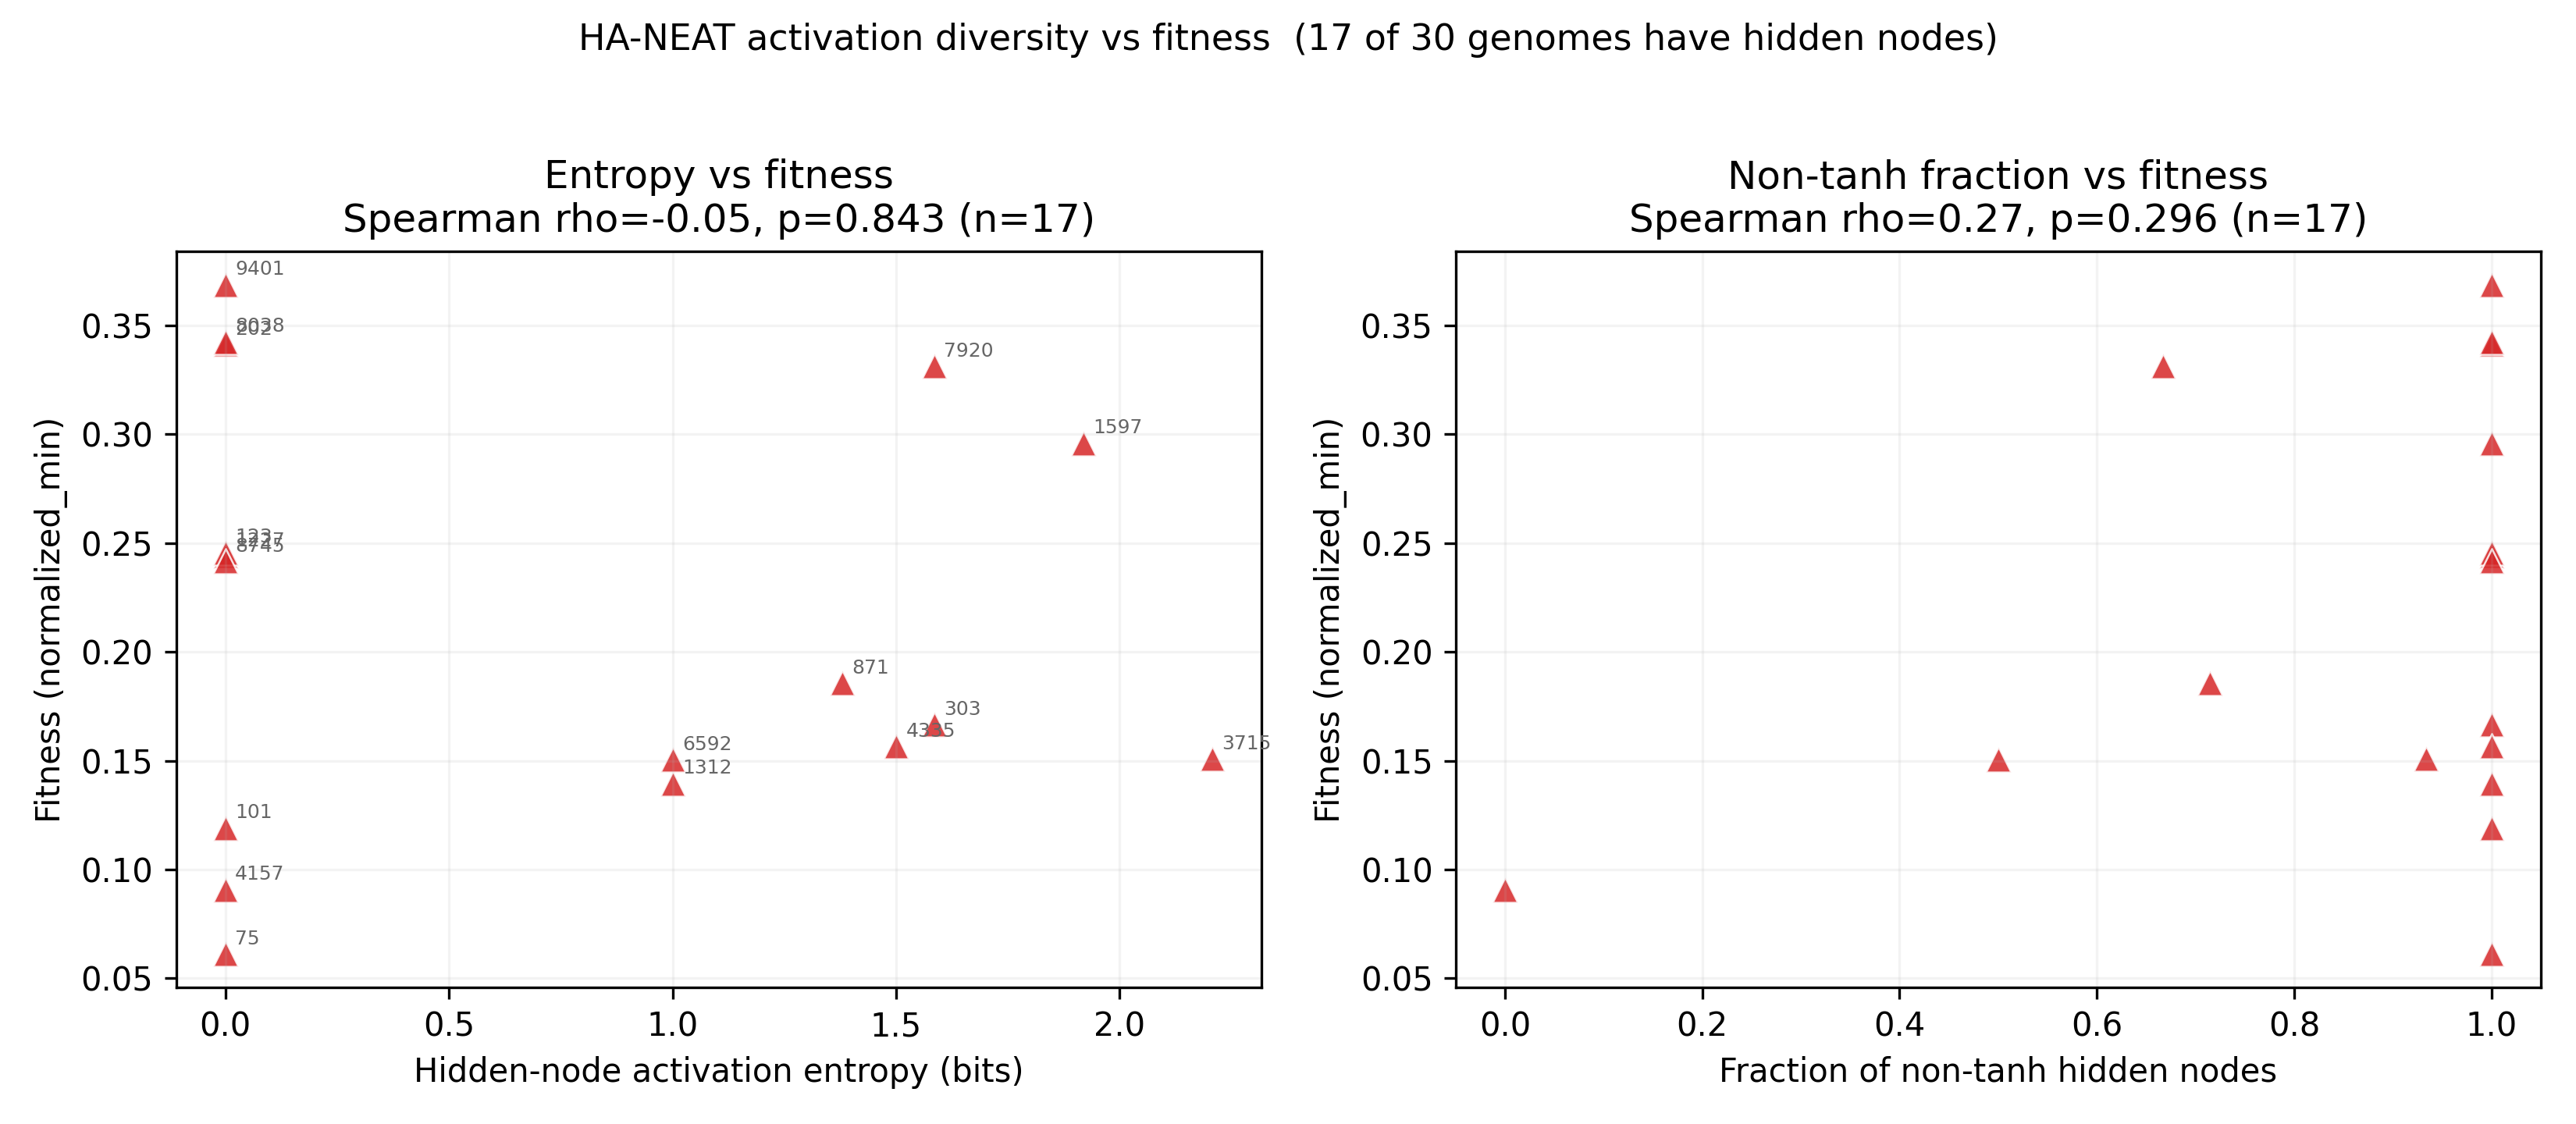
\includegraphics[width=\textwidth]{Figures/activation_entropy_vs_fitness.png}
\textit{(b) Activation entropy vs.\ fitness ($n=17$).}
\label{fig:pop200-activation-fit}
\end{minipage}
\caption{Activation usage within HA-NEAT champions in the pop200 study. (a) Diversity is genuinely
exploited (tanh is the least common activation at 11\%), but (b) neither entropy nor non-tanh
fraction predicts fitness across the 17 champions with hidden nodes.}
\FloatBarrier
\end{figure}

\subsection{Discussion of the pop200 analyses}
\label{sec:pop200-discussion}

Activation diversity did not raise multi-task fitness.
The HA-NEAT machinery still left a structural signal that the fitness comparison alone would have missed.
The three analyses in this section were exploratory, run only after the pre-registered fitness comparison returned a null result, and we read them as hypothesis-generating.

The clearest structural signal is that NEAT champions carried more hidden nodes than the ablation's, even though the two reached the same fitness.
A naive ``NEAT with one activation'' expectation predicts the opposite, which suggests the ablation does not behave like standard NEAT.
The ablation runs the HA-NEAT mutation operator.
Even with a tanh-only activation set, the activation-mutation event still fires and still reassigns the historical markers on every connection of the chosen hidden node.
The activation change is a functional no-op (tanh to tanh), yet the marker side effect persists: reassigned markers register as disjoint genes in the compatibility distance and degrade crossover alignment for any genome carrying hidden nodes.
We hypothesize that this suppresses the spread of hidden-node structures.
That account would explain why the ablation tracks HA-NEAT, and not NEAT, in the node counts, and it would locate the compactness effect in the HA-NEAT machinery instead of in activation diversity.
We stress that this mechanism is a hypothesis.
It is consistent with the code path and with the observed ordering, but we did not test it directly, and the effect is small and rests on a single significant pairwise contrast.

Within HA-NEAT, the evolved networks used the full activation set and did not collapse back to tanh, so the diversity mechanism is genuinely exercised.
Even so, we detected no relationship between activation diversity and fitness, which is consistent with the headline null: on this task the lever HA-NEAT provides is pulled, and pulling it does not move fitness.
The per-task analysis suggests why the task may be insensitive to that lever.
In every condition the champions saturated Hopper at a low plateau and were bottlenecked by Walker2D.
Once Hopper already exceeds Walker2D, the normalized-minimum objective makes further Hopper gains selectively invisible.
We therefore read the effective optimization problem as degenerating toward ``improve Walker2D subject to keeping Hopper alive.''
That regime exerts far less genuine multi-task pressure than the two-task framing implies, and it leaves little room for any mechanism to distinguish itself.

These analyses have clear limitations.
First, the hidden-node comparison rests on very small, heavily tied counts (medians of 0--2 hidden nodes), which weakens the rank test and inflates the influence of a few large genomes; the significant NEAT-versus-ablation contrast should be read as suggestive.
Second, the species-count comparison is uninformative because all conditions saturate the configured species ceiling, so this design cannot test whether HA-NEAT's speciation protection sustains more diversity.
Third, the Hopper plateau confounds the multi-task claim: because Walker2D is almost always the binding task, the study measures single-task Walker2D optimization more than true multi-task pressure.
Fourth, the activation-fitness correlations rest on only 17 informative genomes and are underpowered.
Fifth, all of these results come from a single population size (200), so the structural effects may not persist at other scales.

Three concrete follow-ups would address these limitations directly.
The marker-reassignment hypothesis is testable with a targeted ablation that sets the activation-mutation rate to zero while keeping the rest of the HA-NEAT machinery: if the compactness effect is caused by marker reassignment, it should disappear.
Restoring genuine multi-task pressure calls for either a harder first task or a different aggregation that does not clip improvements on the leading task, such as the normalized product, so that both tasks remain under selection throughout.
Finally, repeating the complexity and activation analyses at larger population sizes would test whether the structural differences observed here are scale-dependent.
None of these fit the remaining compute budget and are left to future work.




\section{Conclusion and Future Work}
We have

\clearpage \printbibliography

\end{document} 
